%%%%%%%%%%%%%%%%%%%%%%%%%%%%%%%%%%%%%%%%%%%%%%%%%%%%%%%%%%%%%%%%%%%%%%%%%%%%%%%%
% data_set.tex:
%%%%%%%%%%%%%%%%%%%%%%%%%%%%%%%%%%%%%%%%%%%%%%%%%%%%%%%%%%%%%%%%%%%%%%%%%%%%%%%%
\chapter{Search Analysis for Long-Lived Particles }
\section{Analysis Strategy}
This analysis searches for delayed isolated photons produced with large transverse momentum. From a theoretical point of view, events containing such a photon will be a clear signal for new physics as such a photon is not expected to be produced from standard model interactions. However, from an experimental point of view, using  timing measurements from  ECAL sub-detector, there are many different sources of isolated, hight \pt photons. A few of these sources which have been identified are high \pt isolated and delayed photons due to timing miss reconstruction and miss-identification, photons produced from cosmic and other beam related effects like beam halo muons bremsstrahlung in the ECAL, and obviously, detector effects like high \pt neutrons by-passing the crystals and hitting directly the photo-detectors like APD and VPT, mimicking the behaviour of isolated, delayed and high \pt photons. The latter kind of photons are called spikes. They are normally isolated, high \pt and their ECAL time measurement show that they arrive early as well as late but with most of them arriving late compared to photons produced at the nominal proton-proton interaction region whose average arrival time at ECAL is 0~ns. These different sources of background makes it a bit challenging to distinguish a possible signal photon from true physics and background photons which are mainly instrumental.
Thus, estimating the background contributions to possible signal sample requires using true proton-proton collision events or data rather than simulated events as is normally done in most physics  analysis. 
Nevertheless, as it is with most hadron collider physics analysis, exploring the use of the number of jets in the event selection can most often reduce dramatically the background contamination to possible signal sample. It is not different with this analysis, as we have employed jet multiplicity both as a physics related quantity for the production of high \pt isolated and delayed photons but also as a detector variable for reducing and at times discriminating  background contribution to possible signal sample.
Our motivation is related to the existence of physics models beyond the SM like the minimal GMSB~(mGMSB) and GGM, where the production of a high \pt isolated, delayed photon in association  with a number of jets constitutes a typical new physics event  which could be produced at the LHC.
Thus using simulated events from mGMSB or GGM model, serves both as a guiding model for the confirmation of a new physics signature at LHC but also as an alternate hypothesis for setting upper limits based on this model in the case that no significant excess over SM prediction is observed.

A typical signal event considered in this analysis for the existence of a neutral massive long-lived particle decaying into a photon is the detection of a late photon arriving at crystals in the ECAL sub-detector of CMS associated with jets with large \MET .  However, the production and decay of this long-lived neutral particle, in our case the neutralino~($\tilde{\chi}^{0}_{1}$), is associated with the production of at least two jets and a weakly interacting gravitino~($\tilde{G}$) as an additional decay product, with a late arrival photon since this is a cascade decay process from a possibly higher mass object into the neutralino and finally to the gravitino. The presence of the gravitino~($\tilde{G}$) is inferred using the transverse momentum imbalance whose magnitude is \MET .
In the  SPS8 minimal GMSB or GGM model with R-parity conservation~(RPC) assumed, SUSY particles are  produced in pairs and so there would be an event having at least a single photon arriving late, associated with at least 2 jets and large \MET . This signal configuration helps in defining and selecting our signal region~(SR) and a control region~(CR) for estimating the contribution to this signal from standard model processes and the detector effects considered as background processes.
\subsection{Signal and Background Modelling}
The SPS8 GMSB and GGM signal event generation begins with the production of Supersymmetry Les Houches Accord~(SLHA) files using the SUSY ISASUSY package written by \cite{Baer}  containing the ISAJET software. The SUSY events are forced to decay according to the SPS8 GMSB and GGM model using the SDECAY decay package. These SLHA files containing information about the SUSY mass spectrum and decay rates is passed through a PYTHIA 6 \cite{pythia6} interface into the CMS software~(CMSSW), in this case CMSSW532patch7, where proton-proton collision at $\sqrt{8}$~TeV events producing SUSY particles events are generated. Their interaction with the CMS detector is simulated using the GEANT4 package \cite{geant4}. Standard Model processes like  multi-jets and $\gamma +$ jets processes produced from strong interactions described by quantum chromodynamics~(QCD) are generated and simulated at leading order cross-sections using PYTHIA 6 and GEANT4 packages respectively.
Digitisation and event reconstruction in terms of its constituent objects like jets, photons, muons and electrons, after its passage and decay in the full CMS detector is later performed still using the CMSSW software.
\subsubsection*{Signal}
The SPS8 mGMSB possible new physics parameter space used for the present physics analysis involves: $\tan\beta = 15$, $sign(\mu) = 1$, and $M_{m} = 2.\cdot \Lambda_{m}$. While $c\tau$ and $\Lambda_{m}$ is used to scan the available parameter space which maximises the sensitivity of the CMS detector to long-lived particles, in this scenario mostly neutralinos~($\tilde{\chi}^{0}_{1}$). The cascade decay of higher mass SUSY particles in the SUSY spectrum to $\tilde{\chi}^{0}_{1}$ allows for signal events with the following constituents:
\begin{itemize}
\item at least one energetic photon,
\item large missing transverse momentum,
\item a number of high transverse momentum jets.
\end{itemize}
\subsubsection*{Background}
QCD multi-jets and $\gamma +$ jet(s) events produced in leading order cross-sections with high \pt range of the photons, serves as background and also for time reconstruction and calibration and for sanity check. Events with $W$  and $Z$ decay  and $t\bar{t}$ with large missing transverse momentum are also generated for serving as sanity check for understanding momentum measurements.
\subsection{Datasets}
The proton-proton collision dataset used in this analysis was collected during 2012 runs at the center of mass energy of  $\sqrt{S} = 8$~TeV  and was collected using the CMS detector giving a total integrated luminosity of 19.1~\fbinv .
\subsubsection*{Data}
The dataset consist is mostly containing events with at least a single photon triggered and only those selected using only luminosity-sections certified as GOOD in the CMS official run file; JASON: \textbf{Cert\_8TeVPromptReco\_Colllisions12\_JASON.txt}. Table \ref{tab:DATA} shows the dataset used in this analysis.

\begin{center}
%\begin{table}[ht]
%\renewcommand\arraystretch{1.2}
\centering
\begin{tabular}{c c}
\hline
Dataset Name & Recorded Luminosity $[\fbinv]$ \\
\hline
 \texttt{/Run2012B/SinglePhoton/EXODisplacedPhoton-PromptSkim-v3 } & 5.1 \\
 \texttt{/Run2012C/SinglePhoton/EXODisplacedPhoton-PromptSkim-v3 } & 6.9 \\
 \texttt{/Run2012D/SinglePhoton/EXODisplacedPhoton-PromptSkim-v3 } & 7.1 \\
\hline\hline
\texttt{/SingleElectron/Run2012A-22Jan2013-v1/AOD} & 5.2 \\
\texttt{/DoubleElectron/Run2012C-22Jan2013-v1/AOD} & 4.8 \\
\hline
\end{tabular}
\captionof{table}{The dataset name and corresponding integrated luminosity of the data used in the analysis}
\label{tab:DATA}
%\end{table}
\end{center}


\subsubsection*{Background and Signal Monte Carlo}
The Monte carlo ~(MC) samples are produced taking into account the Summer 2012 prescriptions carrying information on the calibration and alignment status of the CMS detector with pile up~(PU) conditions at 8 TeV taking into consideration.
 QCD events are generated with a cross -section ($\sigma$) at leading order~(LO) and normalised to the 19.1 \fbinv integrated luminosity. 50112 events were requested for GMSB signal MC, however, due to an observes reduced lifetime ($c\tau$) observed for these official CMS samples, private sample were generated and simulated covering the same line 8 of the SPS8 mGMSB proposal  while the absence of any MC signal samples for GGM model, meant that we had to privately generate our own samples. The SPS8 mGMSB MC samples are generated to scan $\tilde{\chi}^{0}_{1}$ lifetime $c\tau$ from 250~mm to 12000~mm for each $\Lambda_{m}$ point with $\Lambda_{m}$ ranging from $100$~TeV to $180$~TeV and seen in table \ref{tab:mc_GMSB_sample} while  table \ref{tab:mc_QCD_sample} show the \pt range  for the processed QCD samples.

\begin{center}
%\begin{table}[ht]
%\renewcommand\arraystretch{1.2}
\centering
\begin{tabular}{l l l l}
     %\hline
       %\textbf{Signal MC [mGMSB~(SPS8)]}
        \hline
        $\Lambda$~[TeV] & $c\tau$~(mm) & $\sigma_{LO}$~(pb) & Number of events\\
       \hline
       100 & 250-12,000  & 0.368  & 60,000 \\
       120 & 250-12,000  & 0.133  & 60,000 \\
       140 & 250-12,000  & 0.0574 & 60,000 \\
       160 & 250-12,000  & 0.0277 & 60,000 \\
       180 & 250-12,000  & 0.0145 & 60,000 \\
       \hline
       \end{tabular}  
\captionof{table}{The signal GMSB MC samples used in this analysis}
\label{tab:mc_GMSB_sample}
%\end{table}
\end{center}

\begin{center}
%\begin{table}[ht]
%\renewcommand\arraystretch{1.2}
\centering
\begin{tabular}{c c c}
\hline
$\hat{\pt}$ & $\sigma_{LO}$ (pb) & number of events\\
\hline
 50 $\sim$ 80  & 3322.3  & 1995062 \\
 80 $\sim$ 120 &  558.3  & 1992627 \\
120 $\sim$ 170 &  108.0  & 2000043 \\
170 $\sim$ 300 &   30.1  & 2000069 \\
300 $\sim$ 470 &    2.1  & 2000130 \\
470 $\sim$ 800 &  0.212  & 1975231 \\
\hline
\end{tabular}
\captionof{table}{The $\gamma +$ jets samples used in this analysis}
\label{tab:mc_QCD_sample}
%\end{table}
\end{center}

\section{Event Selection}
The major background events to this analysis are events which are not produced from the nominal proton-proton collisions. These events can be put into four major three major categories; \textit{•} Halo Muons}, \textit{Spikes} and \textit{Cosmic muons}.  In addition to these events, there are also QCD events which mimic the $\tilde{\chi}^{0}_{1} \rightarrow \gamma + \tilde{G}$ decay as a result of photon mis-reconstruction and measurement of fake \MET . Along with QCD events, there are also $\gamma + $ jets events as background where there is the presence of a real isolated photon and a fake \MET is expected due to mis-reconstruction of photons from jets. However, the event topology for $\gamma +$ jets is quite different from that of GMSB events. 
\paragraph*{•}
Another interested possible background contribution, in addition to QCD multi-jets events can come from events with electroweak~(EWK) decay. This include $W \rightarrow e + \nu$ decays, $t\bar{t}$ decays, where the top~(t) decays to a $b$ quark and a $W$ 100\% of the time. The electron is mis-reconstructed as a photon and real \MET is measured due to the presence of the neutrinos~($\nu$).  However, most of these EWK and QCD background contributions have very low jet multiplicity in their events and as a result a selection of events with at least two jets helps to reduce their background contribution to a minimal level prior to additional photon quality selections based on the isolation and electromagnetic shower profile which eventually reduces its contribution to non-existent once photon time acceptance of $t_{\gamma} > 3$~ns is applied.

\paragraph*{}
Cosmic muons, beam halo muons and ECAL spikes can all produced photons large reconstructed time and can contribute largely to \MET measurements since they contribute to \MET calculation which normally measures the \pt of all the detected particles in an event assuming all of these events arise from the nominal proton-proton collision although in practice cosmic muons, beam halo muons, spikes, ECAL and HCAL noise can all contribute to the total sum of the measurable event \pt imbalance but arising from non- nominal collision sources. 
A pre-event selection requiring at least a good vertex, 2 or more jets ECAL spike cleaning, DT time cosmic muon cleaning and CSC tight halo-muon cleaning is shown to be very useful in reducing and estimating the contribution of these important background sources.
\subsection{Trigger}
Event selection process begins online using a higher level trigger~(HLT). The HLT trigger used for this analysis during the $\sqrt{S} = 8$~TeV proton-proton collision is the \texttt{HLT\_DisplacedPhoton65\_CaloIdVL\_IsoL\_PFMET25} seeded by \texttt{HLT\_L1SingleEG12} level 1 trigger. This trigger was developed primarily for the study of displaced photons. To avoid bias in event selection towards any particular model, this trigger only requires that an accepted event must have an isolated photon with a \pt threshold of 65~GeV/c and a \MET above 25~GeV. In order to study the trigger efficiency and turn-on curve~( where the event selection efficiency becomes very close to 100\%), we avoid  any correlation between the photon and \MET objects selection, by using a \texttt{SingleMuon} dataset~(\texttt{HLT\_IsoMu30}) to study the efficiency measurements.
The results of the trigger efficiency measurements are shown in figure \ref{fig:HLTEff} against photon \pt and \MET. These efficiency studies are made using the \texttt{HLT\_Photon50\_CaloIdVL\_IsoL} which has no \MET and jet multiplicity requirement  as the denominator and the \newline
\texttt{HLT\_DisplacedPhoton65\_CaloIdVL\_IsoL\_PFMET25} as the numerator. A \texttt{SinglePhoton} dataset is used to verify these efficiency while and GMSB and $\gamma +$ jets samples is used to derive any correction factors between data and MC events.

\begin{center}
\centering
\mbox{
\includegraphics[height=7cm, width=0.5\textwidth]{THESISPLOTS/HLT-EfficiencyVsMET.png}
\includegraphics[height=7cm, width=0.5\textwidth]{THESISPLOTS/HLTEfficiencyVsPhotonpt.png}}
\captionof{figure}{Trigger efficiency turn-on curves for photon \pt and $\MET > 25$~GeV~(left) and for \MET with photon $pt > 80$~GeV/c~(right).}
\label{fig:HLTEff}
\end{center}

\subsection{Offline Selection}
Offline event selection is directed towards selection of displaced photons with very minimal model dependency in terms of event jet multiplicity as possible. As a result, the event selection requires that the event contains at least one photon. The photon collection in contrast to other analysis, which do not employ the use of ECAL timing as a search variable, is extended to include events categorised as being "out-of-time" during the official super cluster reconstruction. These extension even though allows for the inclusion of possible background from spikes, noise, photons from beam hallo and cosmic muons and detector malfunctions also brings with it photons which are potential signal candidates.
The criteria for photon selections can be found in table \ref{tab:PhotonSel}. 

\begin{center}
%\begin{table}[ht]
\centering
\begin{tabular}{c c }
\multicolumn{2}{c}{\bfseries{Photon identification selection criteria}} \\
  \hline 
  \bfseries{Criteria} & \bfseries{Requirement} \\
   \hline 
 % \texttt{primary vertex number of tracks(vnof)}& $>= 4$ \\
 % \texttt{primary vertex transverse distance to beam}~($d0$) & $ < 2$~cm from CMS center \\
%  \texttt{primary vertex longitudinal distance to beam}~($|z|$) & $ < 24$~cm from CMS center \\
  \texttt{Event leading photon must have} $\pt(\gamma^{1})$  & $ > 80$~ GeV \\
  \texttt{Other photons in event must have} $\pt(\gamma^{>1})$  & $ > 45$~ GeV \\
  
 $|\eta_{\gamma}|$,(\texttt{Barrel Only}),  & $ < 3.0$ ($ < 1.5$) \\
 $S_{minor}$  & $ 0.12 \leq S_{Minor} \leq 0.38$ \\
 \textbf{H/E}  & $ < 0.05$ \\
 
 $\Delta R(\gamma, track)$  & $ > 0.6 $ \\
 
 HCAL Iso  & $ < 4.0 $ \\
 ECAL Iso   & $ < 4.5 $ \\
 Track Iso   & $ < 0.2 $ \\
 Photon Isolation cone size $\Delta R(\gamma, other particle)$ & $< 0.4$ \\
 Topological Spike cuts  & $1 - E_{6}/E_{2} < 0.98$, $ 1 - E_{4}/E_{1} < 0.98$ \\ 
  \hline 
\end{tabular}
\captionof{table}{The photon ID selection as used in this analysis}
\label{tab:PhotonSel}
%\end{table}
\end{center}

The presence of the gravitino~($\tilde{G}$) and jets due to the cascade decay~(Feynman diagram in figure \ref{fig:ProdDecay} of section \ref{Science_Chapter}) of the $\tilde{\chi}^{0}_{1} \rightarrow \gamma + \tilde{G}$ decay process as seen in figure \ref{fig:NeutDecay} requires additional selection of jets and \MET.

\begin{center}
\centering
%\mbox{
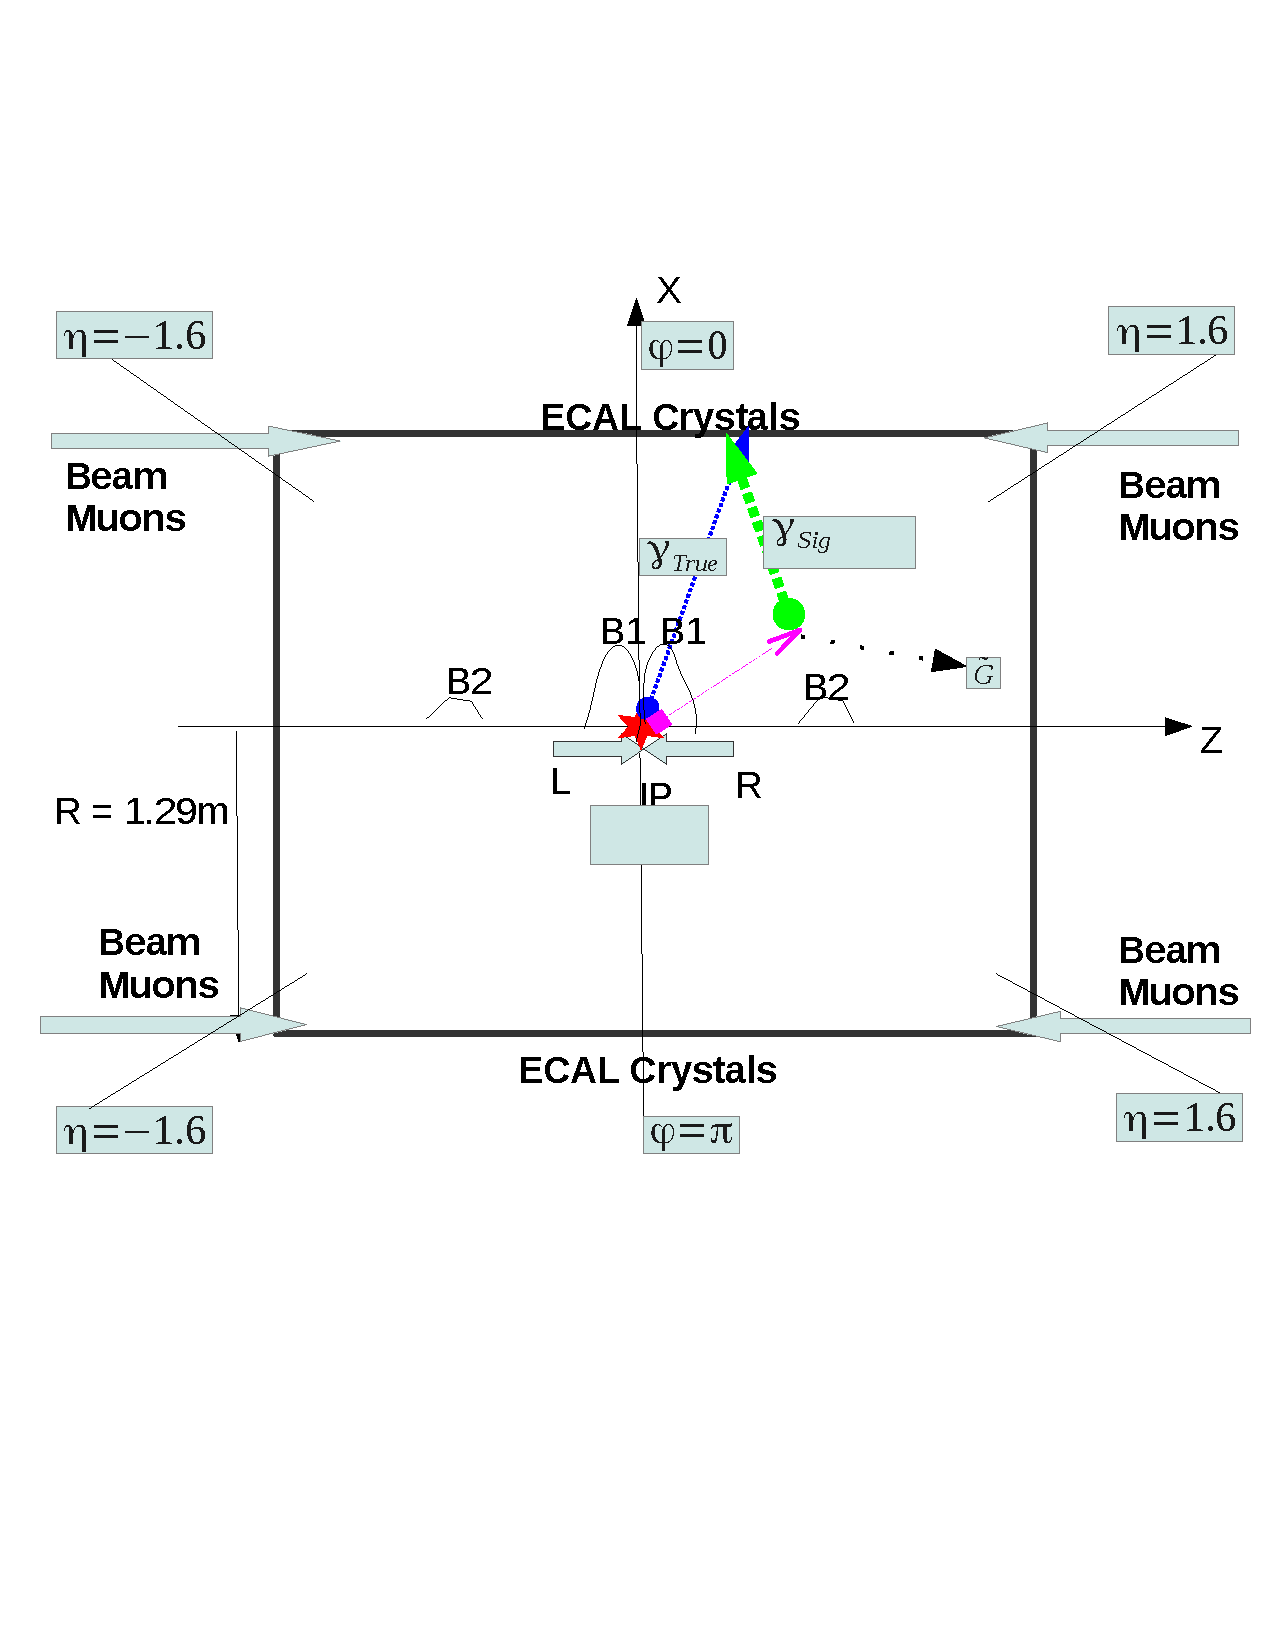
\includegraphics[height=8cm, width=0.8\textwidth]{THESISPLOTS/Background_Delayed_Photon.pdf}
\captionof{figure}{Schematic diagram showing $\tilde{\chi}^{0}_{1} \rightarrow \gamma + \tilde{G}$ decay topology within the ECAL volume of the CMS detector.}
\label{fig:NeutDecay}
\end{center}


The jets and \MET selection criteria are based on the particle-flow algorithm. An additional $\MET > 65$~GeV due to the flatness of the HLT trigger efficiency  against \MET ~( see figure \ref{fig:HLTEff}) while  table \ref{tab:JetSel} summarise the jet identification criteria with threshold requirements used for jet selection in this analysis.

\begin{center}
%\begin{table}[ht]
\centering
\begin{tabular}{c c }
\multicolumn{2}{c}{\bfseries{Jet PF identification selection criteria}} \\
  \hline 
  \bfseries{Criteria} & \bfseries{Requirement} \\
   \hline  
\texttt{Jet} \pt & $ > 35$~GeV \\
 \texttt{Number of Jet constituents} & $ > 1$ \\
 \texttt{Charge EM energy fraction~(CEF) } & $ > 0.99$ \\
 \texttt{Neutral Hadron energy fraction~(NHF) } & $ < 0.99$ \\
 \texttt{Neutral EM energy fraction~(NEF) } & $ < 0.99$ \\
 \texttt{If} $|\eta|$ \texttt{of jet is} $ >2.4$, \texttt{Charge Hadron energy fraction~(CHF) } & $ > 0$ \\
 \texttt{If} $|\eta|$ \texttt{of jet is} $ >2.4$, \texttt{Charge multiplicity~(NCH) } & $ > 0$ \\
 $\Delta R(\gamma, jet) = \sqrt{(\phi_{\gamma}-\phi_{jet})^{2} + (\eta_{\gamma}-\eta_{jet})^{2}}$ & $ > 0.3$ \\
\hline
\end{tabular}
\captionof{table}{The Jet ID selection used in this analysis}
\label{tab:JetSel}
%\end{table}
\end{center}


\subsection{ECAL Time}
In the current analysis, ECAL time of the photon is the main observable and as a result of pile-up contamination with true photons from nominal proton-proton collisions, a reliable definition for the photon time which is robust to pile up.
The two main definitions for ECAL time studied include:
\begin{itemize}
\item Seed Time: Time from the crystal with higher energy in object super cluster which is not a spike.
\item Cluster Time: Error weighted average time of all the crystals in the seed basic cluster of the object super cluster.
\end{itemize} 

The reconstruction of time as described in chapter 4 is extracted from the pulse shape through a fitting method. The $\chi^{2}$ obtained from the fit determines how well the timing is reconstructed. Thus as a means of rejecting fake photons like jets faking photons as well as spikes, a $\chi^{2} < 4 $ cut is applied to improved on the timing resolution and hence improve on the rejection of anomalous photon.
Figure \ref{fig:spikeVsPhoton} shows a comparison between the pulse shape profile of a spike and that of a normal event from data.

\begin{center}
\centering
%\mbox{
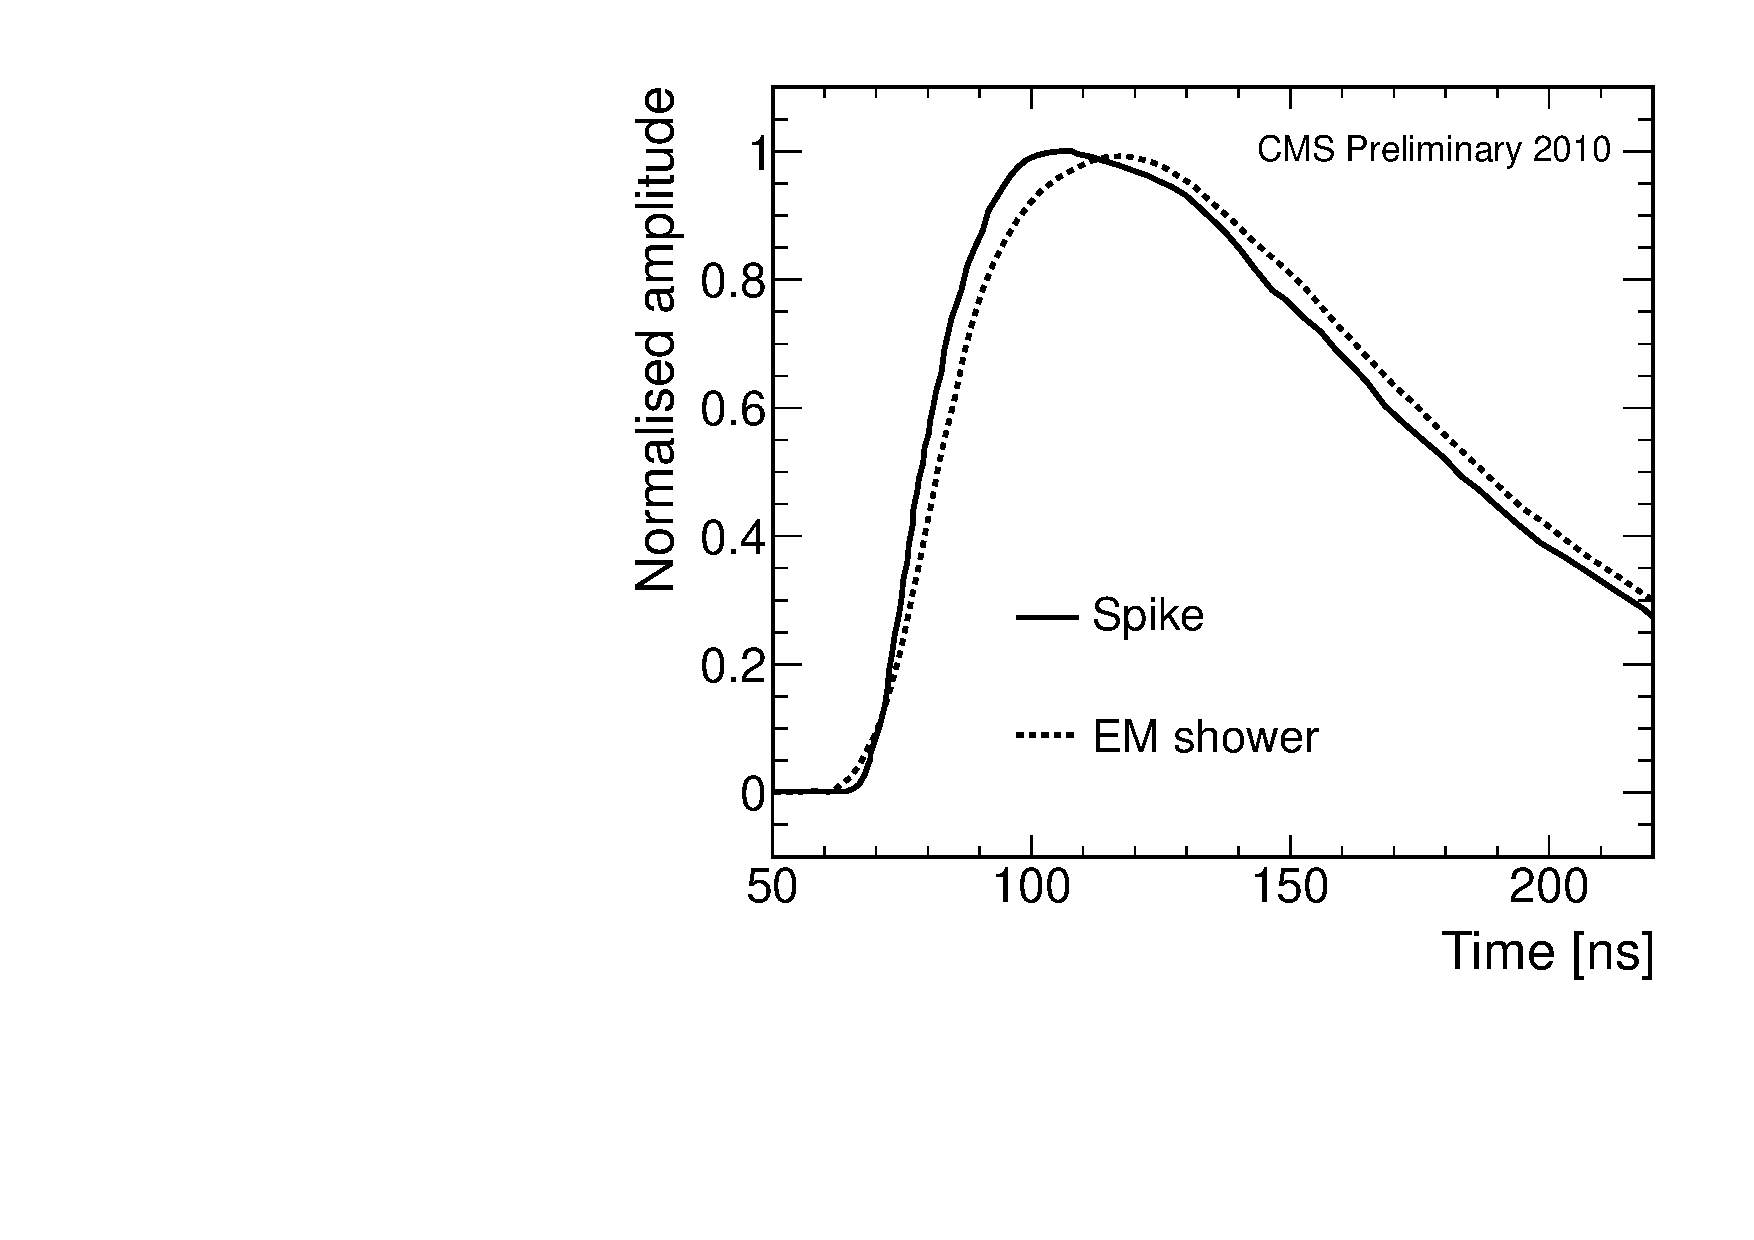
\includegraphics[height=6cm, width=0.7\textwidth]{THESISPLOTS/spike_pulse_shape.pdf}
\captionof{figure}{Pulse shape profile showing a spike~(solid line) and a real photon~(dashed line) from data.}
\label{fig:spikeVsPhoton}
\end{center}.

In a study performed comparing the timing resolution obtained from cluster time to the seed time, it was observed that also the seed time method is very prone to isolated spikes, its resolution especially for large timing events is much better compared to the cluster time measurement method.
Figure \ref{fig:TIME} shows the timing measurements of photons using either seed time or cluster time. The seed time show a timing resolution of $400$~ps compared to $450$~ps with a broad timing tail obtained from using the method of error weighted average cluster time as defined in equation $4.2$ in Timing section.

\begin{center}
\centering
\mbox{
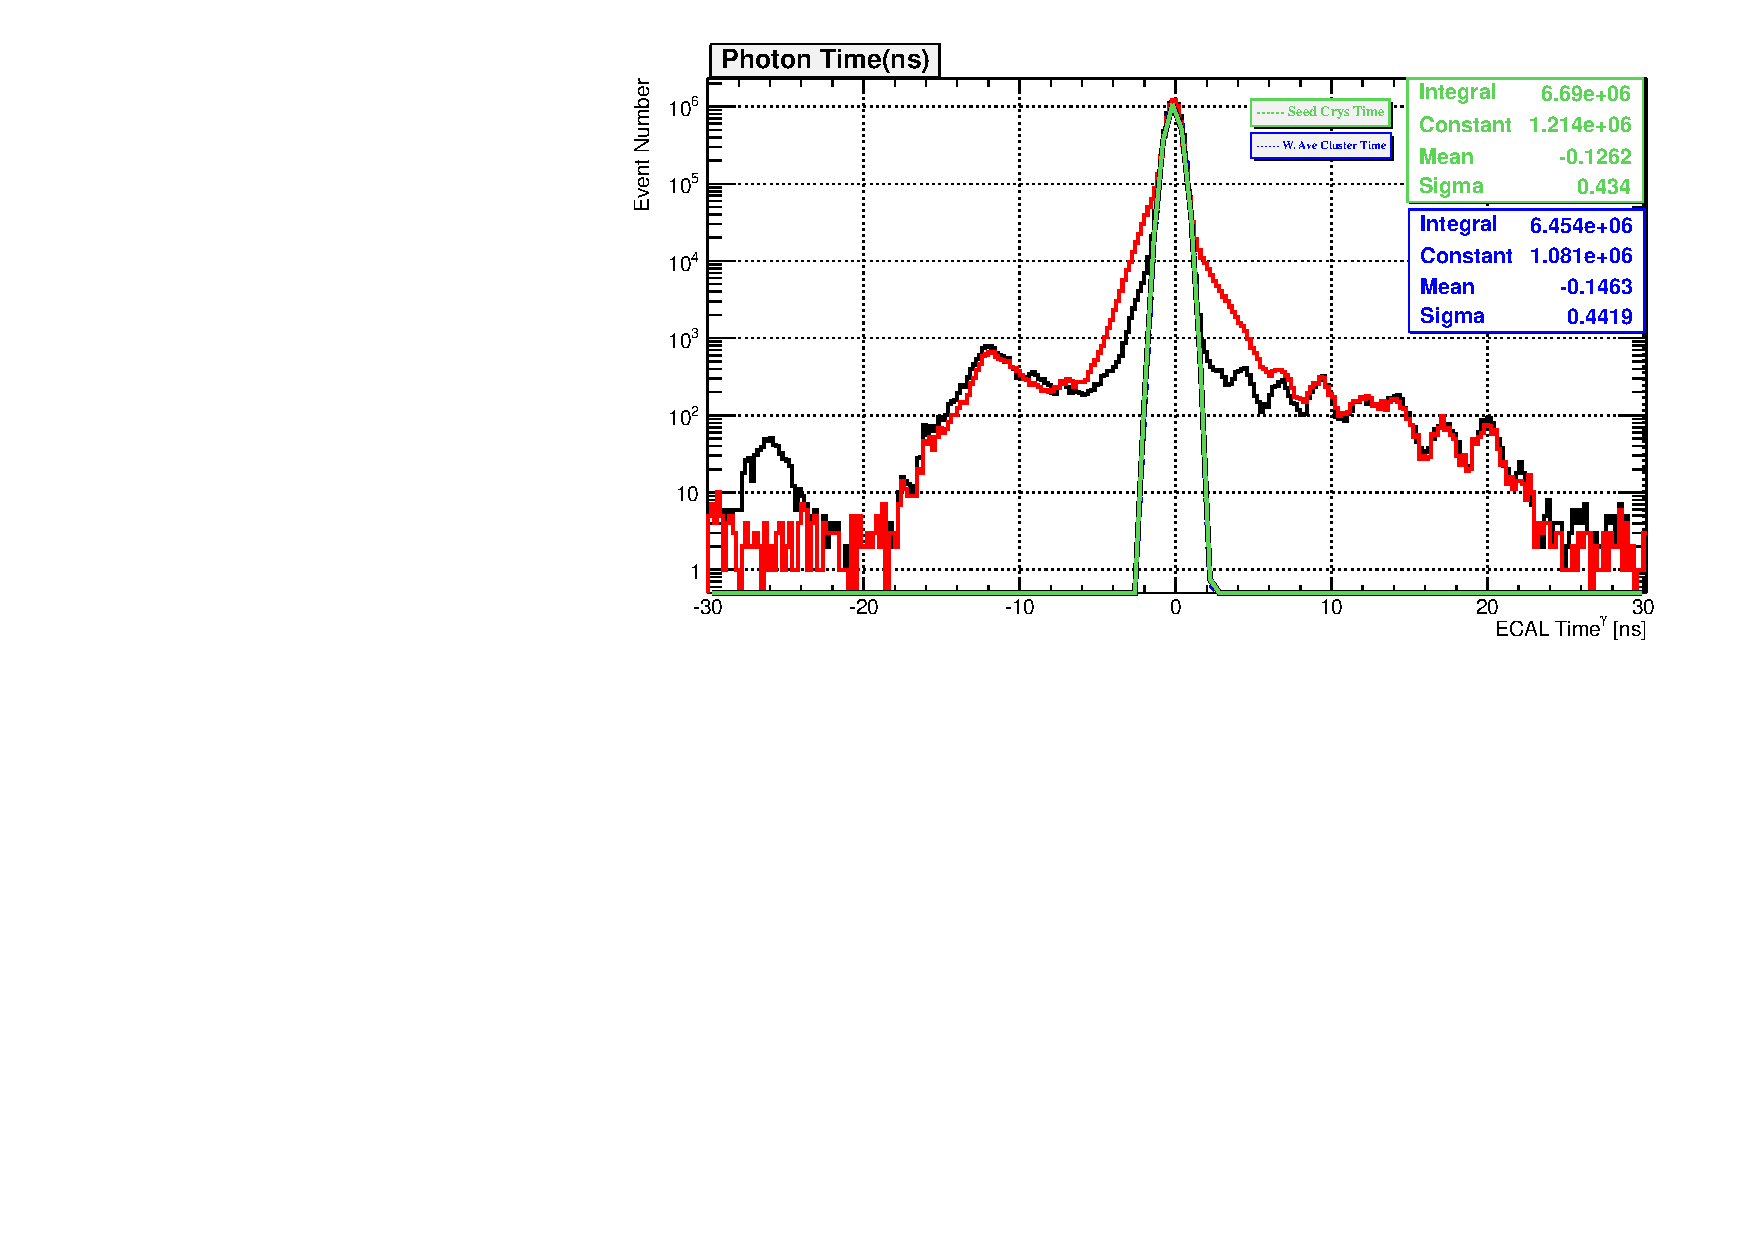
\includegraphics[height=6cm, width=0.5\textwidth]{/home/tensr/Documents/TEN-HEP-PHD-THESIS/PHD_THESIS/PHD/THESISPLOTS/SeedTimeVsWAveBasicClusterTimeDefinitions.pdf}
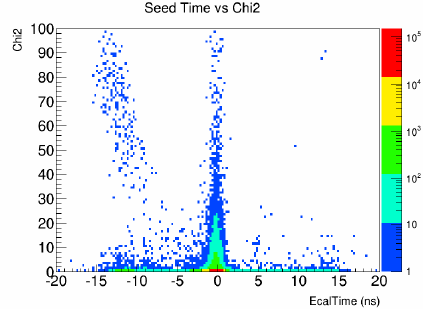
\includegraphics[height=6cm, width=0.5\textwidth]{THESISPLOTS/Seed-Time-Chi2.png}
}
\captionof{figure}{Timing distribution of photons  showing timing measurements using seed crystal~(black) and that using Weighted Average basic cluster time~(blue). Resolution~($\sigma$) from seed time is better compared to that for cluster time. Together with the $\chi^{2}$, the seed time performs better in identifying anomalous timing objects.}
\label{fig:TIME}
\end{center}

Monte Carlo simulation of ECAL timing is very challenging due to the presence of anomalous signals like spikes in data which are not available in MC samples.  Thus in order to study the timing resolution between MC and data, we select events containing only one or two jets and compare this timing distribution to the difference between the Generated time~$(T_{GEN}$) and the MC reconstructed time~($T_{RECO}$) within a timing window of [-2, 2 ]~ns. The difference in peak or mean time between the data and MC $\gamma +$ jet sample is used to smear the reconstructed time of the MC samples to be as comparable to true reconstructed time of data. A difference of about 125~ps is observed between the timing from data and that of MC, and a smearing of of the MC sample shows a close agreement between the smeared reconstructed time of the MC sample to that of data.
Figure \ref{fig:DATAMCTime} shows the this comparison before and after timing calibration~(adjustment) is applied on the MC samples.

\begin{center}
\centering
\mbox{
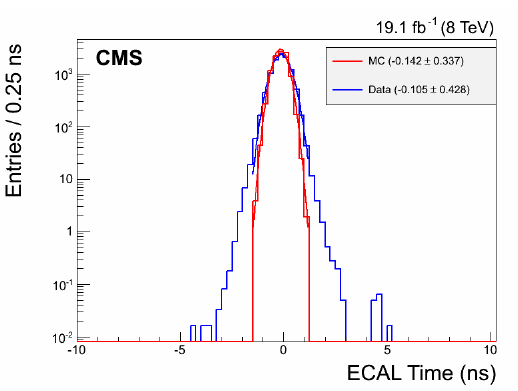
\includegraphics[height=6cm, width=0.5\textwidth]{THESISPLOTS/MC_Vs_DataTimeB4Calib.png}
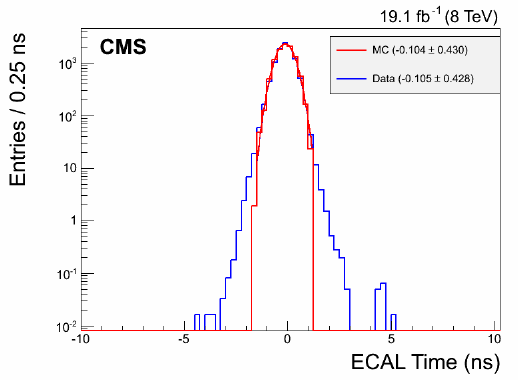
\includegraphics[height=6cm, width=0.5\textwidth]{THESISPLOTS/MC_Vs_DataTimeAferCalib.png}
}
\captionof{figure}{Timing distribution of photons showing timing of data and MC $\gamma +$ jets~(blue) samples and Data~(red) before~(left) and after~(right) timing Calibration is applied to MC.}
\label{fig:DATAMCTime}
\end{center}

It is worth noting that the difference of 125~ps between $T^{MC}_{RECO}$ and $T^{DATA}_{RECO}$ compared to 500~ps ECAL timing resolution is not enough to influence event selection, however event distribution in the tails remains a major concern.
\paragraph*{}
The ECAL timing distribution for photons with $pt > 50$~GeV in the ECAL~(barrel and endcap inclusive i.e $|\eta_{\gamma}| < 3.0$) show timing distributions~(see figure \ref{fig:TIMEECAL})

\begin{center}
\centering
\mbox{
%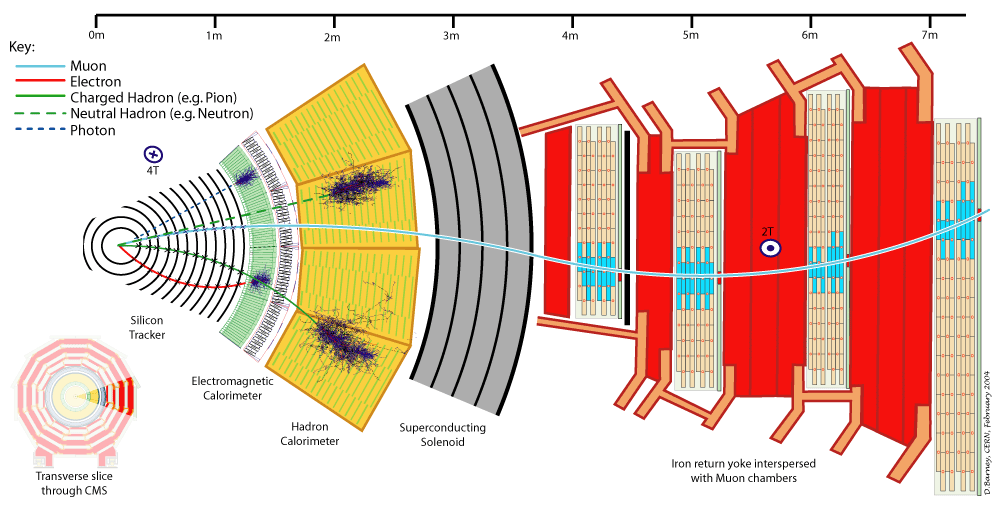
\includegraphics[scale=0.2]{THESISPLOTS/CMS_Slice.png}
%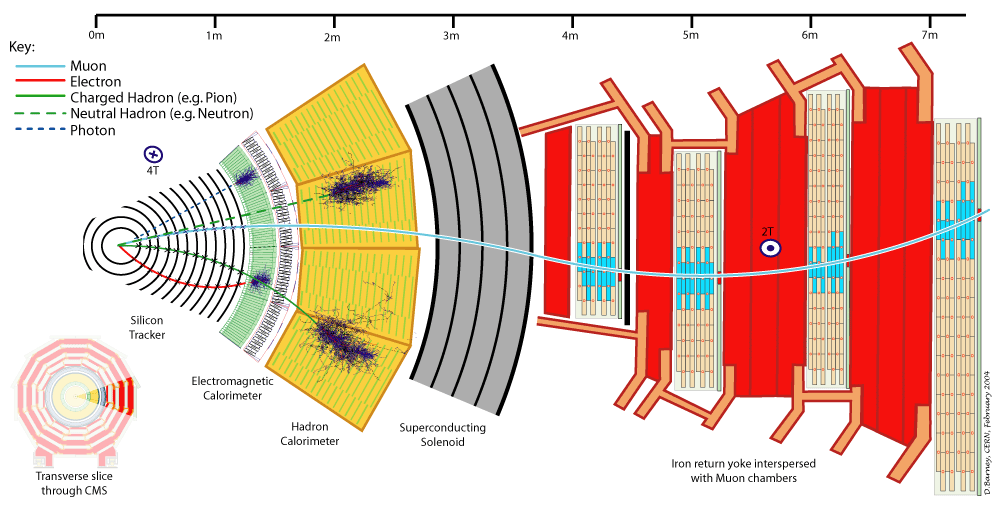
\includegraphics[scale=0.2]{THESISPLOTS/CMS_Slice.png}
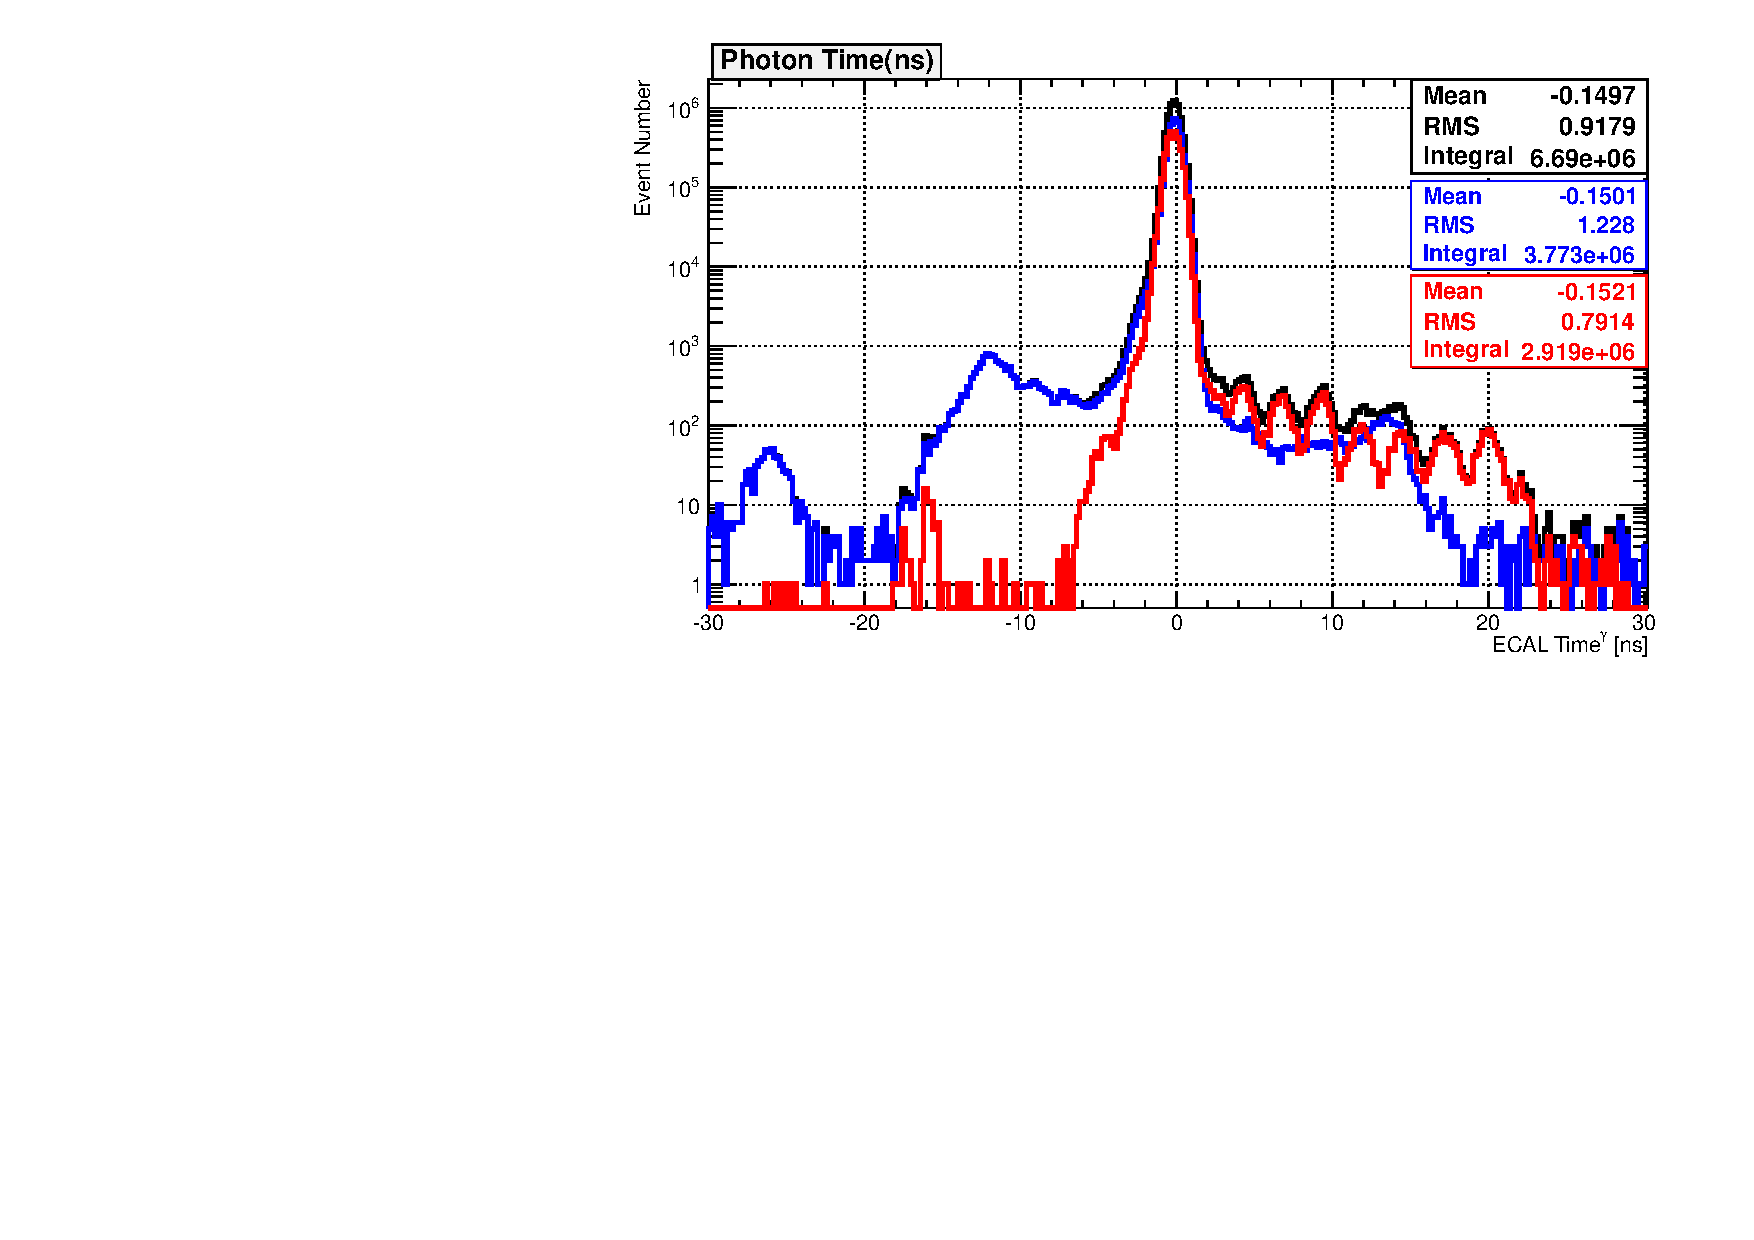
\includegraphics[height=8cm, width=0.9\textwidth]{THESISPLOTS/PhotonECALTimePtMTH50-C-D-SinglePhotonDataset.pdf}
}
\captionof{figure}{ECAL timing distribution of photons in barrel~(\textcolor{blue}{EB}), endcap~(\textcolor{red}{EE}) and all of ECAL~(\textcolor{black}{ALL ECAL}) with $\pt > 50$~GeV from data. A $2.5$~ns delay timing structure is observed in endcap subdetector.}
\label{fig:TIMEECAL}
\end{center}

with a clear 2.5~ns repeated discrete pattern with most of these photons arriving in the endcap, $ 1.47 < \eta < 3.0$ compared to the barrel, $|\eta| < 1.47$. These are photons originating from collisions of \textit{Ghost} and \textit{Satellite} bunches with either the main proton collision bunch or \textit{Ghost}/\textit{Satellite}. They contribute an irreducible amount to the photon time distribution which is very challenging to reject or estimate quantitatively. A rough estimate can be obtained by looking at ratio of the proton population in the filling profile of the LHC RF cavities as mentioned in section 3.1.5 of chapter 3 which gives a factor $10^{-5}$ compared to contributions from the main proton proton collision. It is observed that their main contribution is towards the endcap crystals as very few photons from these secondary collisions are produced with enough \pt compared to those from main proton bunch collisions. And even if they do, the ratio of photons from these secondary proton collision to that of the main proton-proton collision has an upper bound of  $10^{-5}$. 
Thus, the endcap is not used in this analysis for the reason that these contributions is more in the endcap and the timing resolution in the endcap is relatively poor compared to that of the barrel.
The assumption of the upper bound of $10^{-5}$ is verified and validated using events with $Z\rightarrow e^{+}e^{-}$ as $Z$ events must be produced from main proton-proton collisions rather than  ghost/satellite collisions by studying electron candidates with time within [-2.0, 2.0]~ns window. This will be explain in detail in the background estimation section which follows.


\section{Background Estimation}
A better understanding of the different background contributions to the photon ECAL time is shown using a two dimensional histogram of the photon $\eta$ and $\phi$ against the photon seed time and the timing distribution for different jet multiplicity events. Thus the general event selection only requires that the event has at least a photon satisfying the photon selection of the previous section.
The photon ECAL time inclusive distribution plots are shown in figure \ref{fig:BKGPLOTS}

\begin{center}
\centering
\mbox{
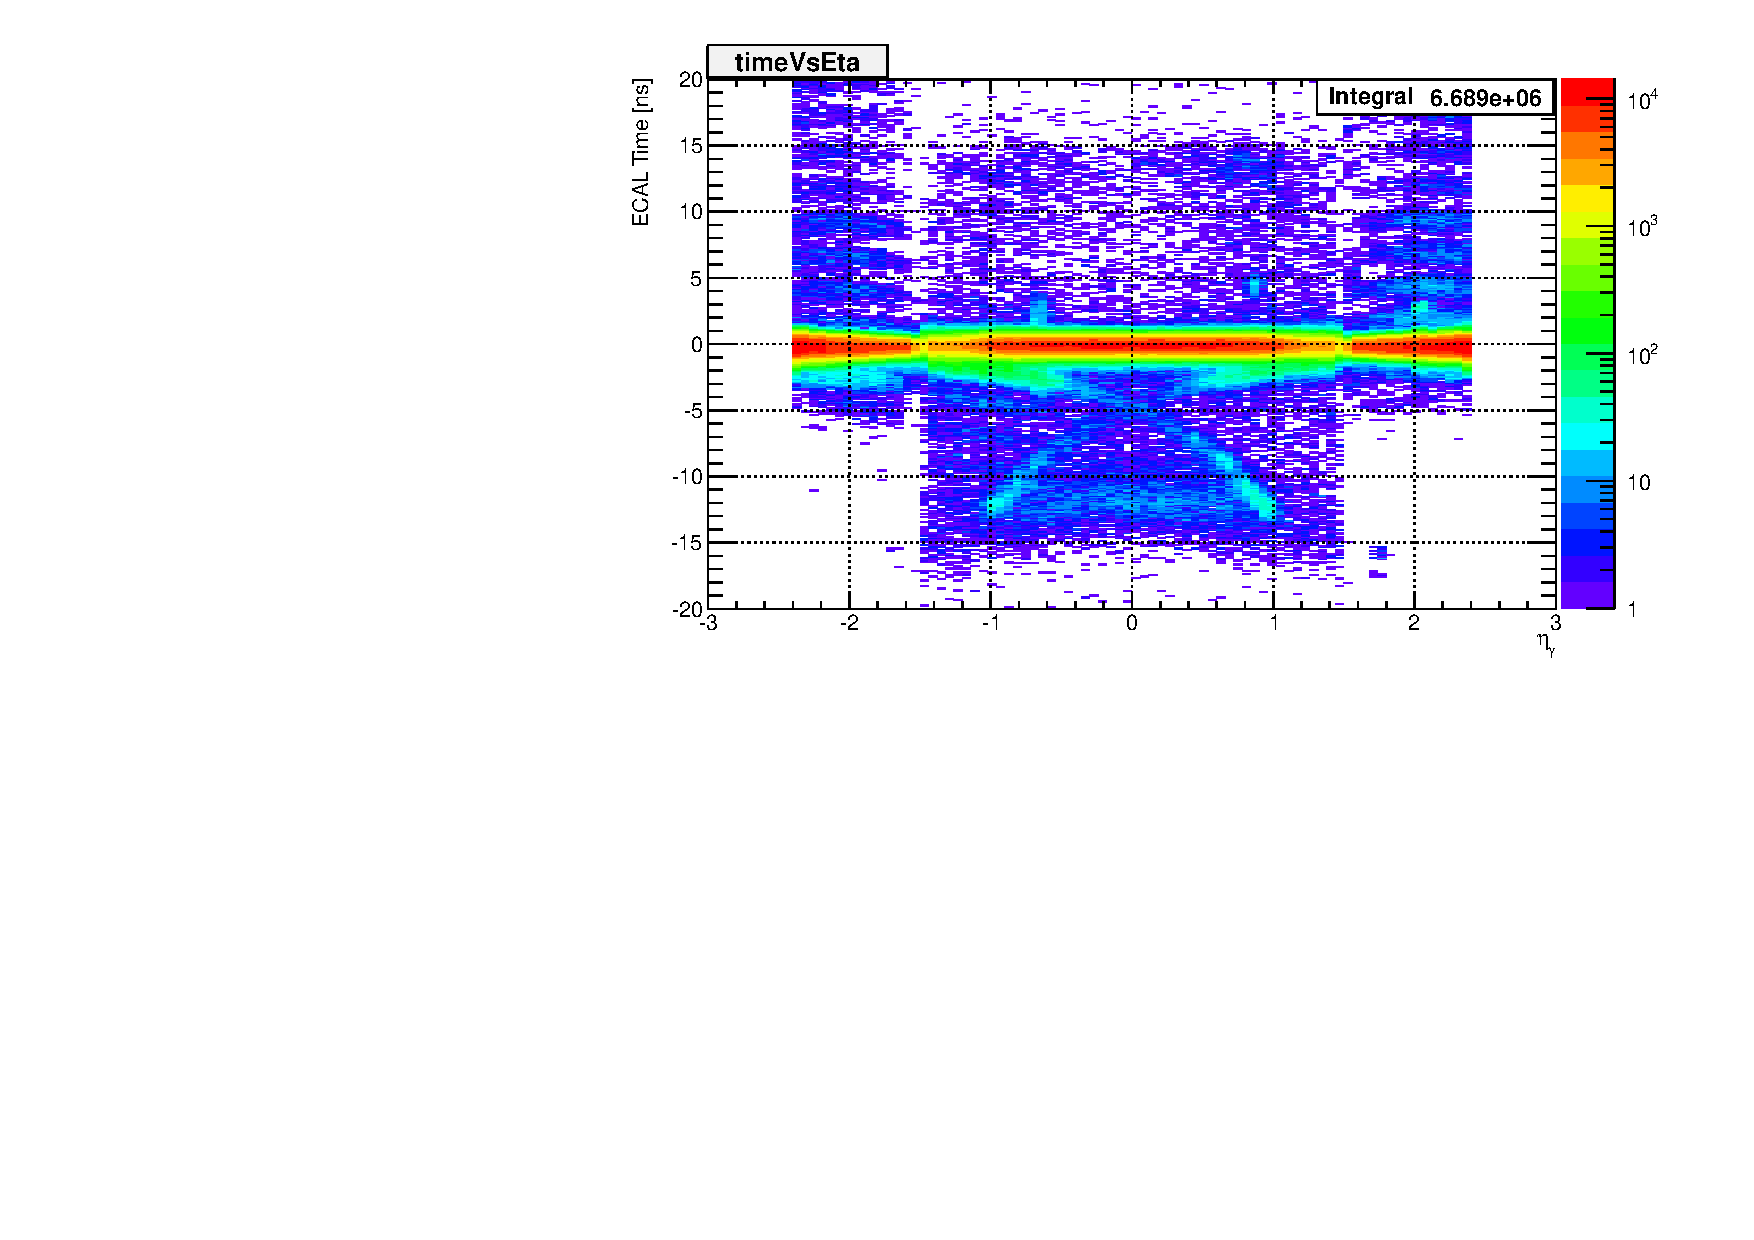
\includegraphics[height=6cm, width=0.5\textwidth]{THESISPLOTS/SinglePhotonDataSet-TimeVsEta.pdf}
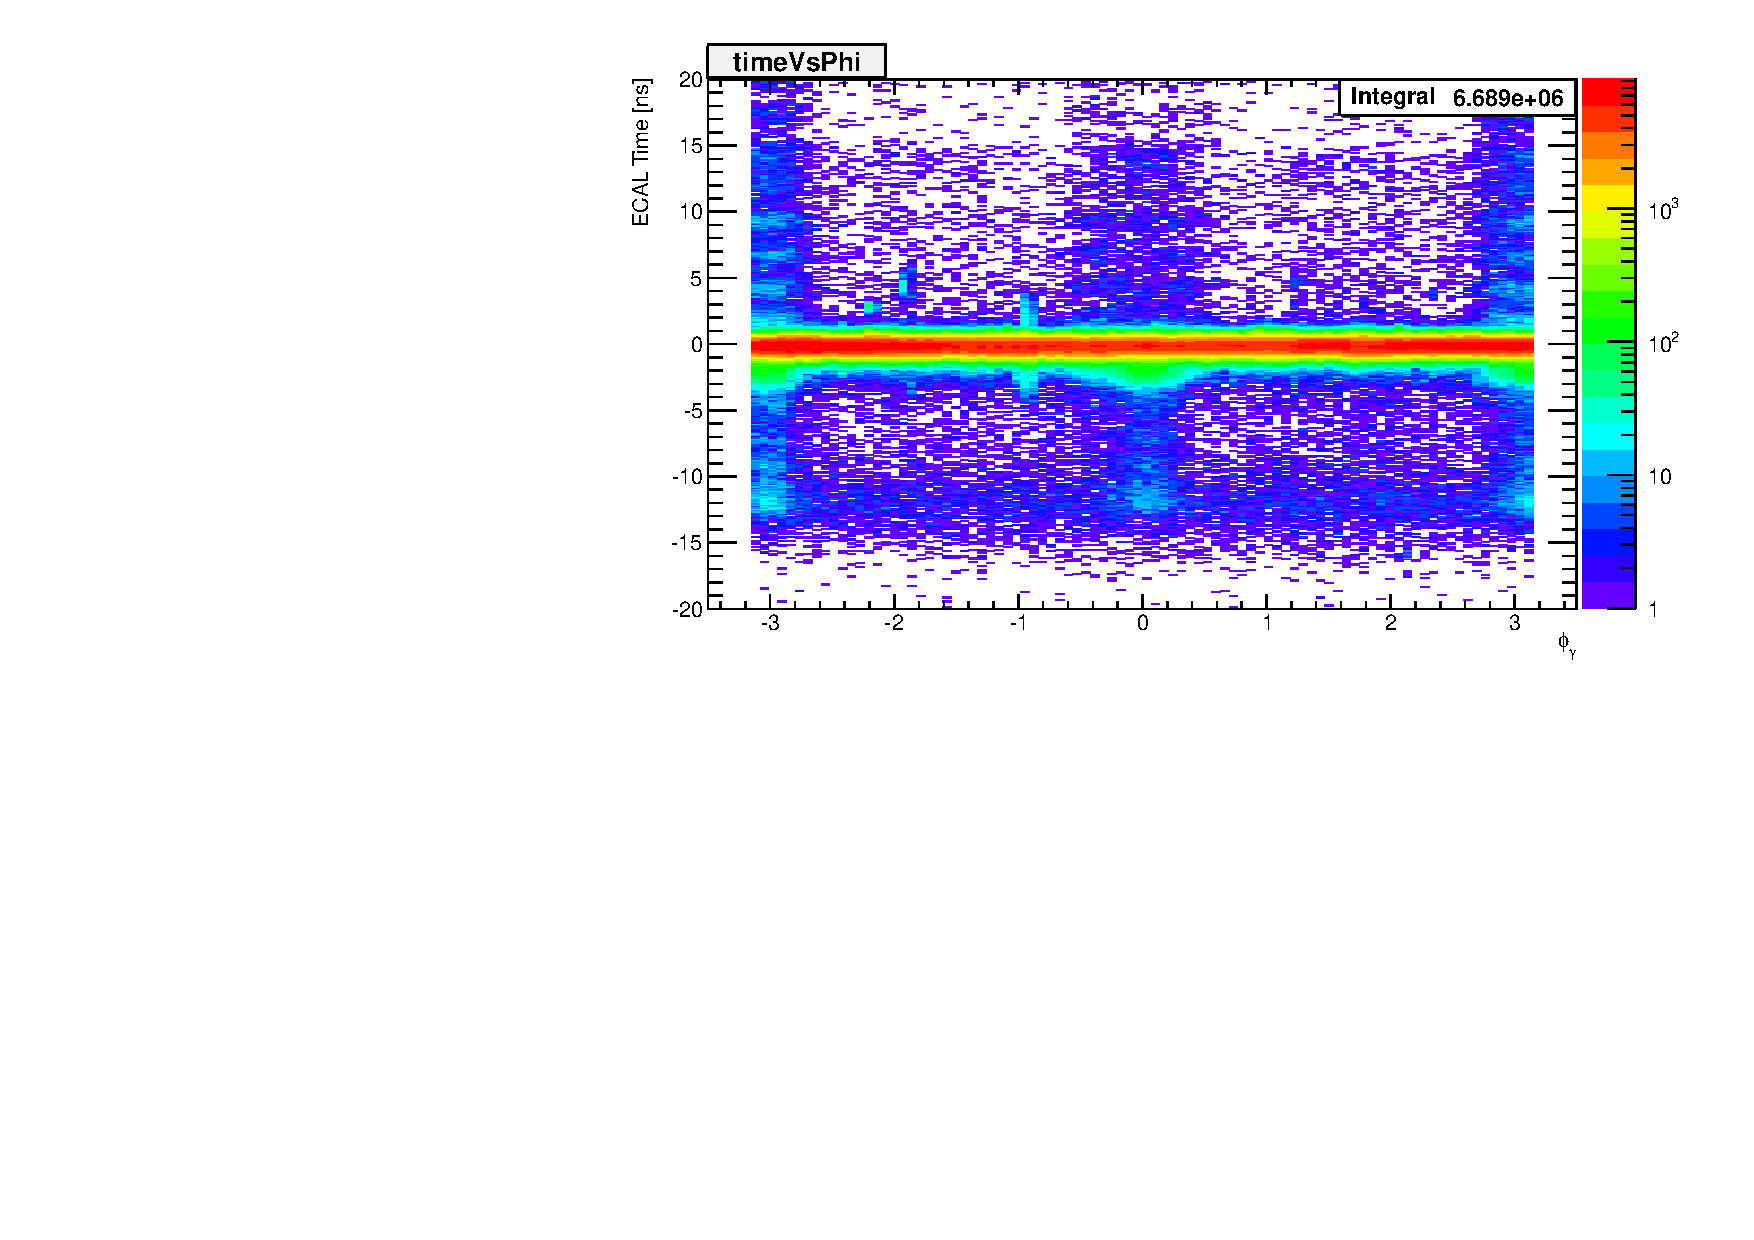
\includegraphics[height=6cm, width=0.5\textwidth]{THESISPLOTS/SinglePhotonDataSet-TimeVsPhi.pdf}}
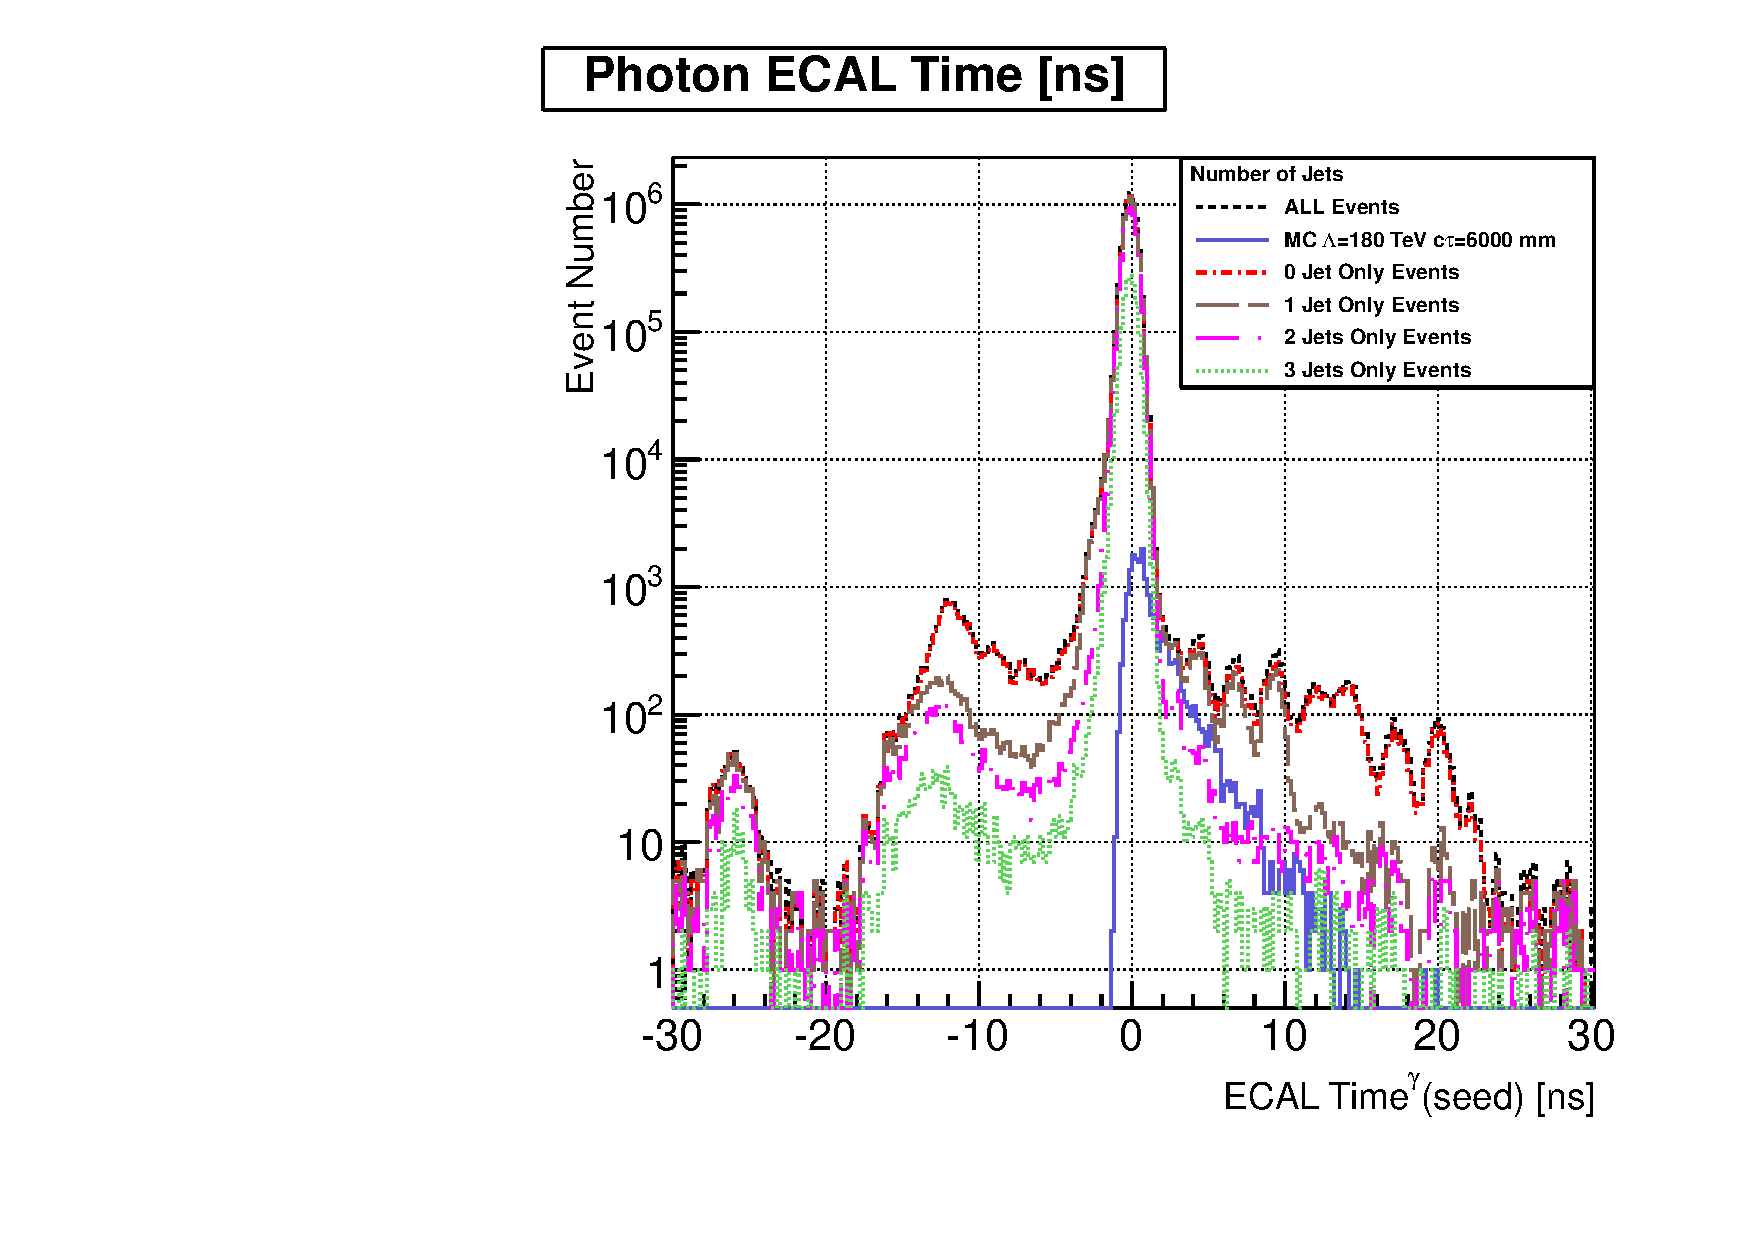
\includegraphics[height=8cm, width=0.8\textwidth]{THESISPLOTS/Photon_SeedXtalTime_Distribution_VsJetMultiplicity.pdf}
\captionof{figure}{ECAL time against $\eta$~(left) and ECAL time against $\phi$~(right) for photons with $\pt > 60$~GeV from data. The lower plot shows the photon timing distribution for events with different jet multiplicity.}
\label{fig:BKGPLOTS}
\end{center}
From the above distributions, there seems to be contributions from quite a variety of sources. The possible sources considered in this analysis include: QCD processes  which we consider to be a combination of $\gamma + $jets, multi-jets and other processes producing photons from nominal bunch collisions. Most QCD processes are expected to have minimal contribution to large timing photons and \MET with their only contributions arising from timing miss-reconstruction and \MET miss-measurements due to miss-identification of jets as photons. Events with possible or true large ECAL time with significant contributions arise from machine induce backgrounds~(MIB)(arising from ghost/satellite bunch collisions), Halo muons, cosmic muons and anomalous events like spikes. These events bring significant contributions to both large photon times and large \MET where which is our possible signal sample.
Thus, the data driven background estimation technique employed in this analysis is as follows:

\begin{itemize}
\item Divide the dataset into individual samples peculiar to the expected kinematics and observation of each individual background source,
\item Identify observable based on its kinematics which can be used as variables to identify or tag and reject a particular background contribution with an acceptable amount of efficiency,
\item Used alternate samples particular to each background source to calculate and verify the event tagging and miss-tag rate or efficiency,
\item Use the tagging and miss-tag rates to estimate the background contribution of each individual background source in a well defined control region~(CR) or sample,
\item Use another CR as a closure test sample to verify our background estimation method.
\end{itemize}

Due to a larger contribution of ghost/satellite bunch collisions observed in the endcap~(EE)(see figure \ref{fig:TIMEECAL}) and poor timing resolutions~($\approx 3.0$~ns), the endcap is not used in this analysis. Thus events are selected if the photon in the event is in the barrel i.e $|\eta_{\gamma}| < 1.47$.

In order to study the background in a data driven method, we divide the dataset into two major samples: Nominal or in-time photons whose photon ECAL time is within $\pm 1$~ns and the event must have at least 2 jets,  and Off-timing photons where the photon ECAL time is $ > 2$~ns but $ < -3$~ns with the event containing no jets. Our motivation is simply because the probability of a MIB or non-collision background producing an event with high jet multiplicity is small  and even reduces with the \pt of of the resulting photon increases while nominal photons are mostly produced in association with jets due to the nature of QCD interactions and are mostly in-time.

By comparing these two samples, we can understand the difference and similarities between collision and non-collision backgrounds. 

\subsection{Non-Collision Backgrounds}
\subsubsection{Halo Photons}
Energetic muons (energy up to 1 TeV) produced in Beam-induced backgrounds~(BIB) as a result of proton losses $z = 150$~m from the interaction point of the CMS detector and inelastic proton interaction with residual gas inside the beam pipe bremsstrahlung in ECAL crystals producing photons with very high \pt and significantly large ECAL time. The rate of these BIB depends on the beam current and the operational conditions of the LHC which include machine optics, collimator settings, residual gas densities and filling scheme. These muons which travel in a near parallel direction to normal protons in the beam pipe, referred to as halo muons are expected to leave a muons tracks  in the Endcap muon systems with a corresponding associated ECAL electromagnetic cluster in the ECAL. They are also peculiar in that they travel from one side of the detector to the other along the $z$-direction, and their  Time-Of-Flight~(TOF) with respect to a potential hit position in the ECAL sub-detector can be estimated as well as measured.
The expected time at ECAL of a  halo muon traveling parallel along the beam line is given using a simple expression given as:

\begin{equation}
t^{\mbox{expected}}_{\mbox{ECAL}} = -1/c\left( \pm Z_{\mbox{cluster}} + \sqrt{Z^{2}_{\mbox{cluster}} + R^{2}_{\mbox{cluster}}}  \right)
\end{equation}

and $\eta$ dependence on this expression showing the different potential hit positions of the muons in ECAL can be seen by re-expressing this same expression in terms of $\eta$ and $\phi$ as:
\begin{equation}
t^{\mbox{expected}}_{\mbox{ECAL}} = - \frac{R_{\mbox{cluster}}}{2c} \exp{(-\eta)}
\end{equation} 

where, $Z$ is the cluster position or longitudinal distance along $z$-axis from nominal interaction point, $R$ is the radial distance of the cluster from the beam line; $R^{EB}_{\mbox{cluster}} = 1.29$~m and $C$ is the speed of light.

With this expression compared to the value from data,we select a sample (figure \ref{ fig:HALO}) to study the halo properties in the negative timing distribution. 
Additional identification of halo muons can be performed using the the Cathode Strip Chambers~(CSC) and the ECAL calorimeter information, Since halo muons are not bent in the azimuthal direction by the magnets and mainly located around the $y=0$ plane, measuring the difference in $\phi$ between the CSC segment position and the ECAL photon cluster. A matching of these two referred to as $CSC(Seg,\gamma)\Delta\phi$ to within $3\deg$ (figure \ref{fig:HALO}) appears to provide a clear distinction between Halo photons and true photons from collision.

A distribution of the Halo photon time against the photon $\phi$ shows that most halo photon are distributed around $\phi = 0, \pm \pi$ as expected.

\begin{center}
\centering
\mbox{
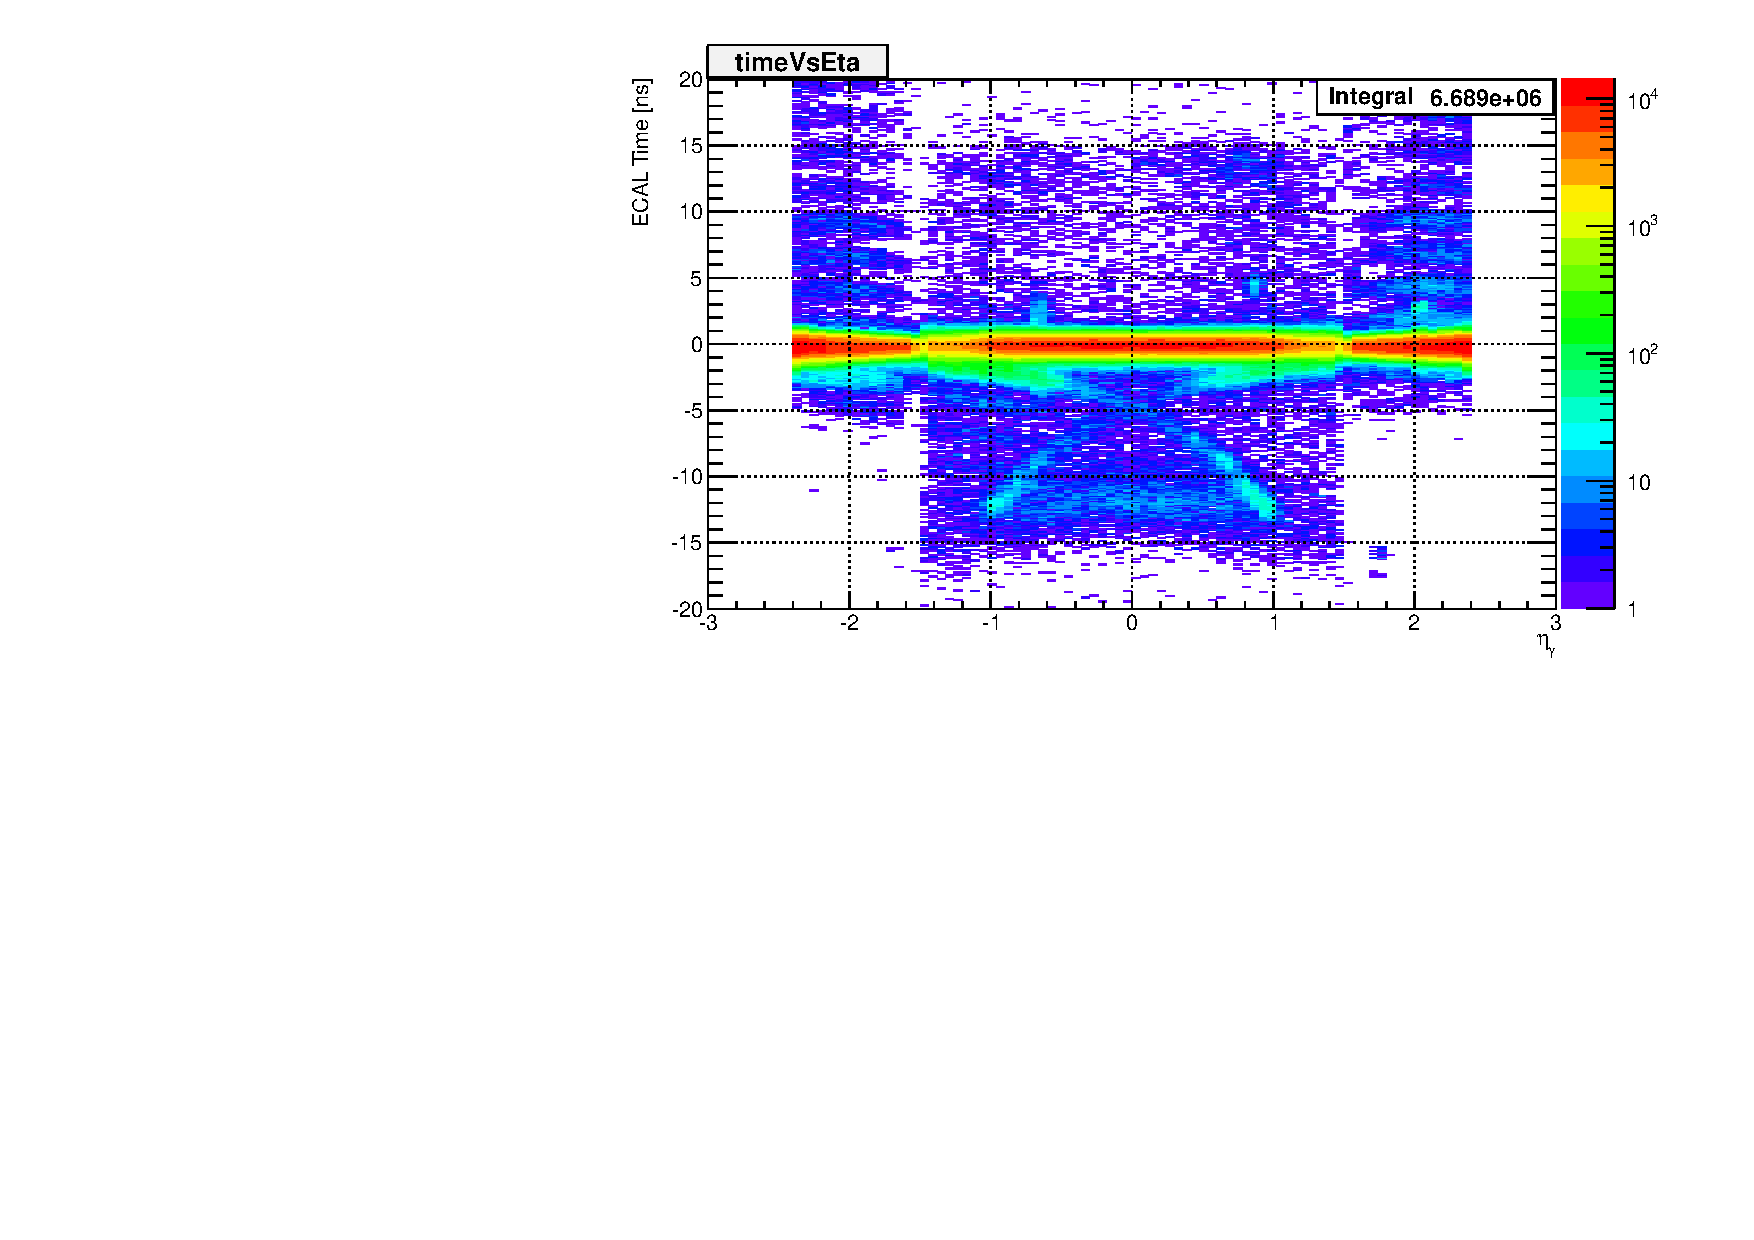
\includegraphics[height=6cm, width=0.5\textwidth]{THESISPLOTS/SinglePhotonDataSet-TimeVsEta.pdf}
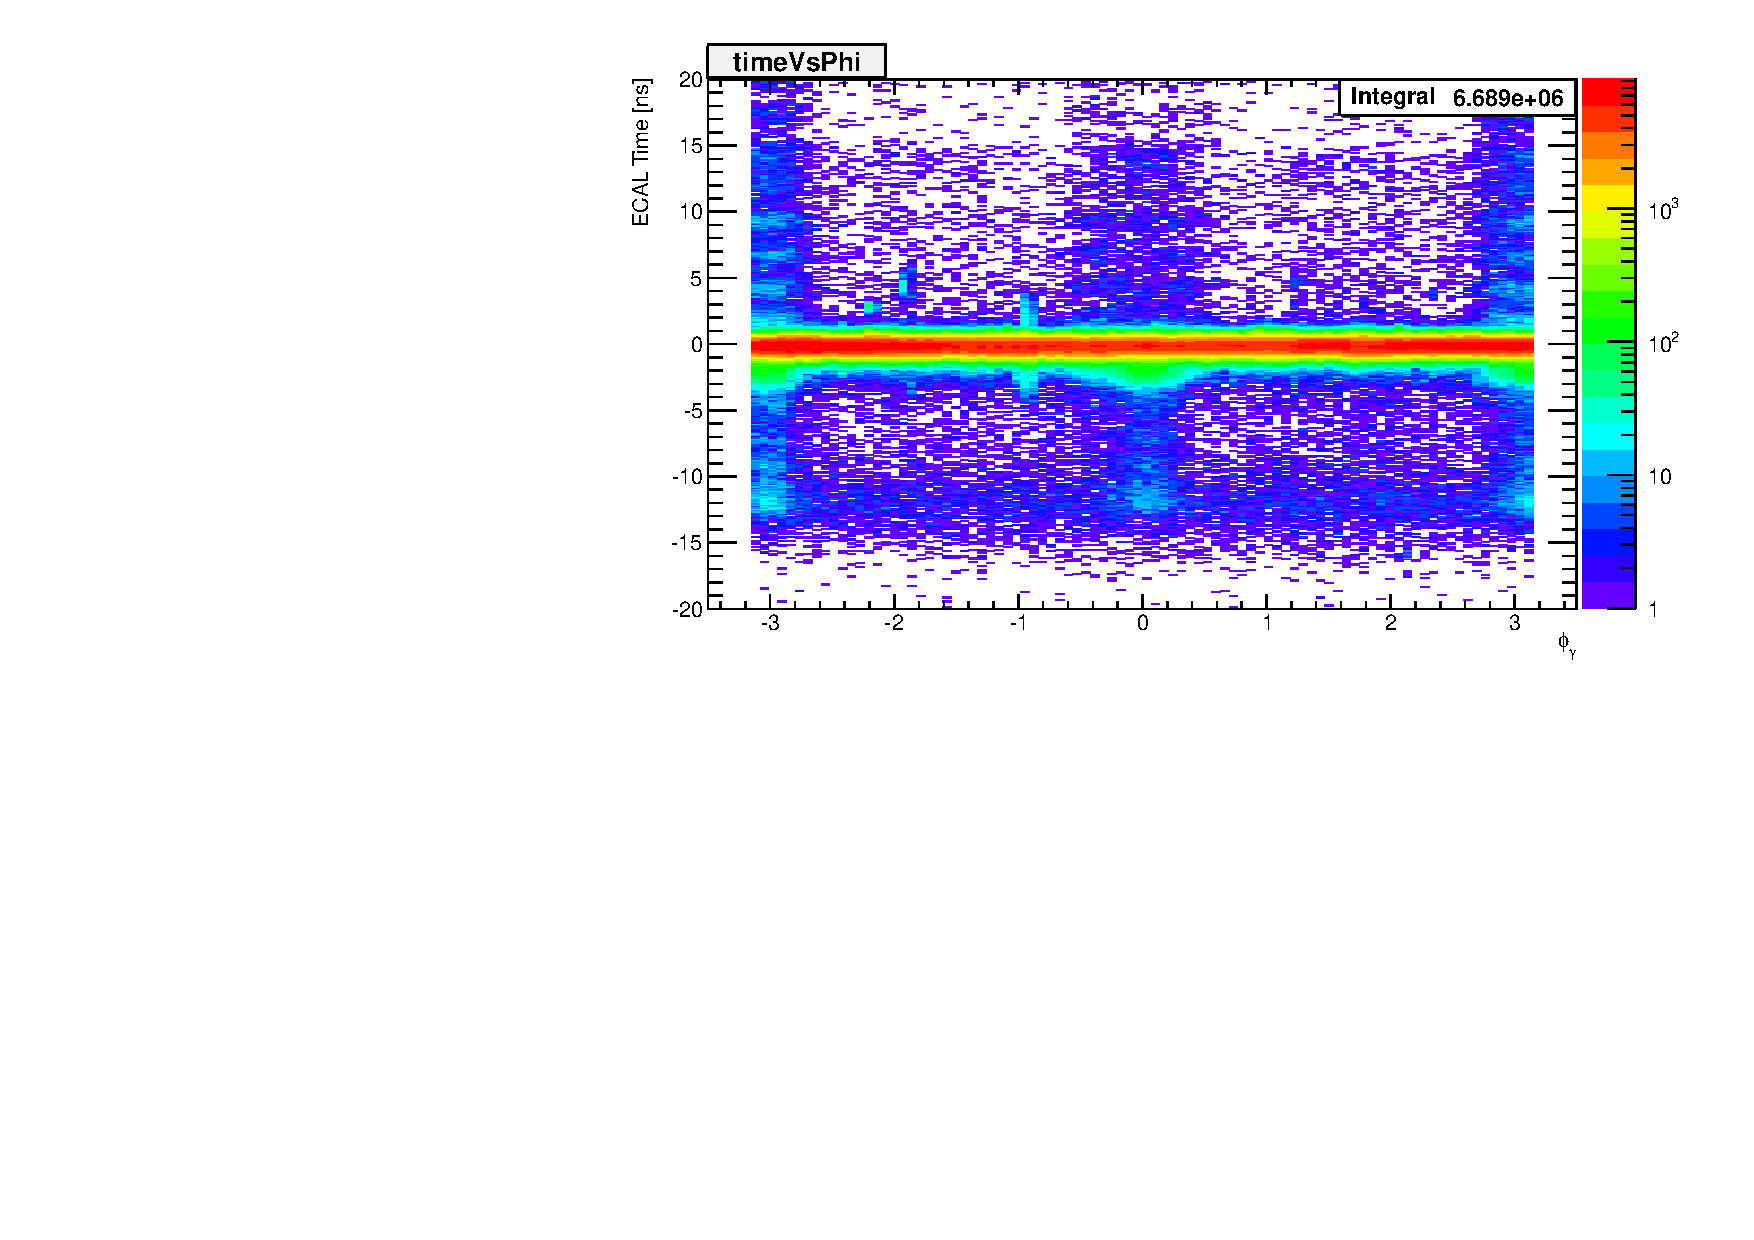
\includegraphics[height=6cm, width=0.5\textwidth]{THESISPLOTS/SinglePhotonDataSet-TimeVsPhi.pdf}}
\mbox{
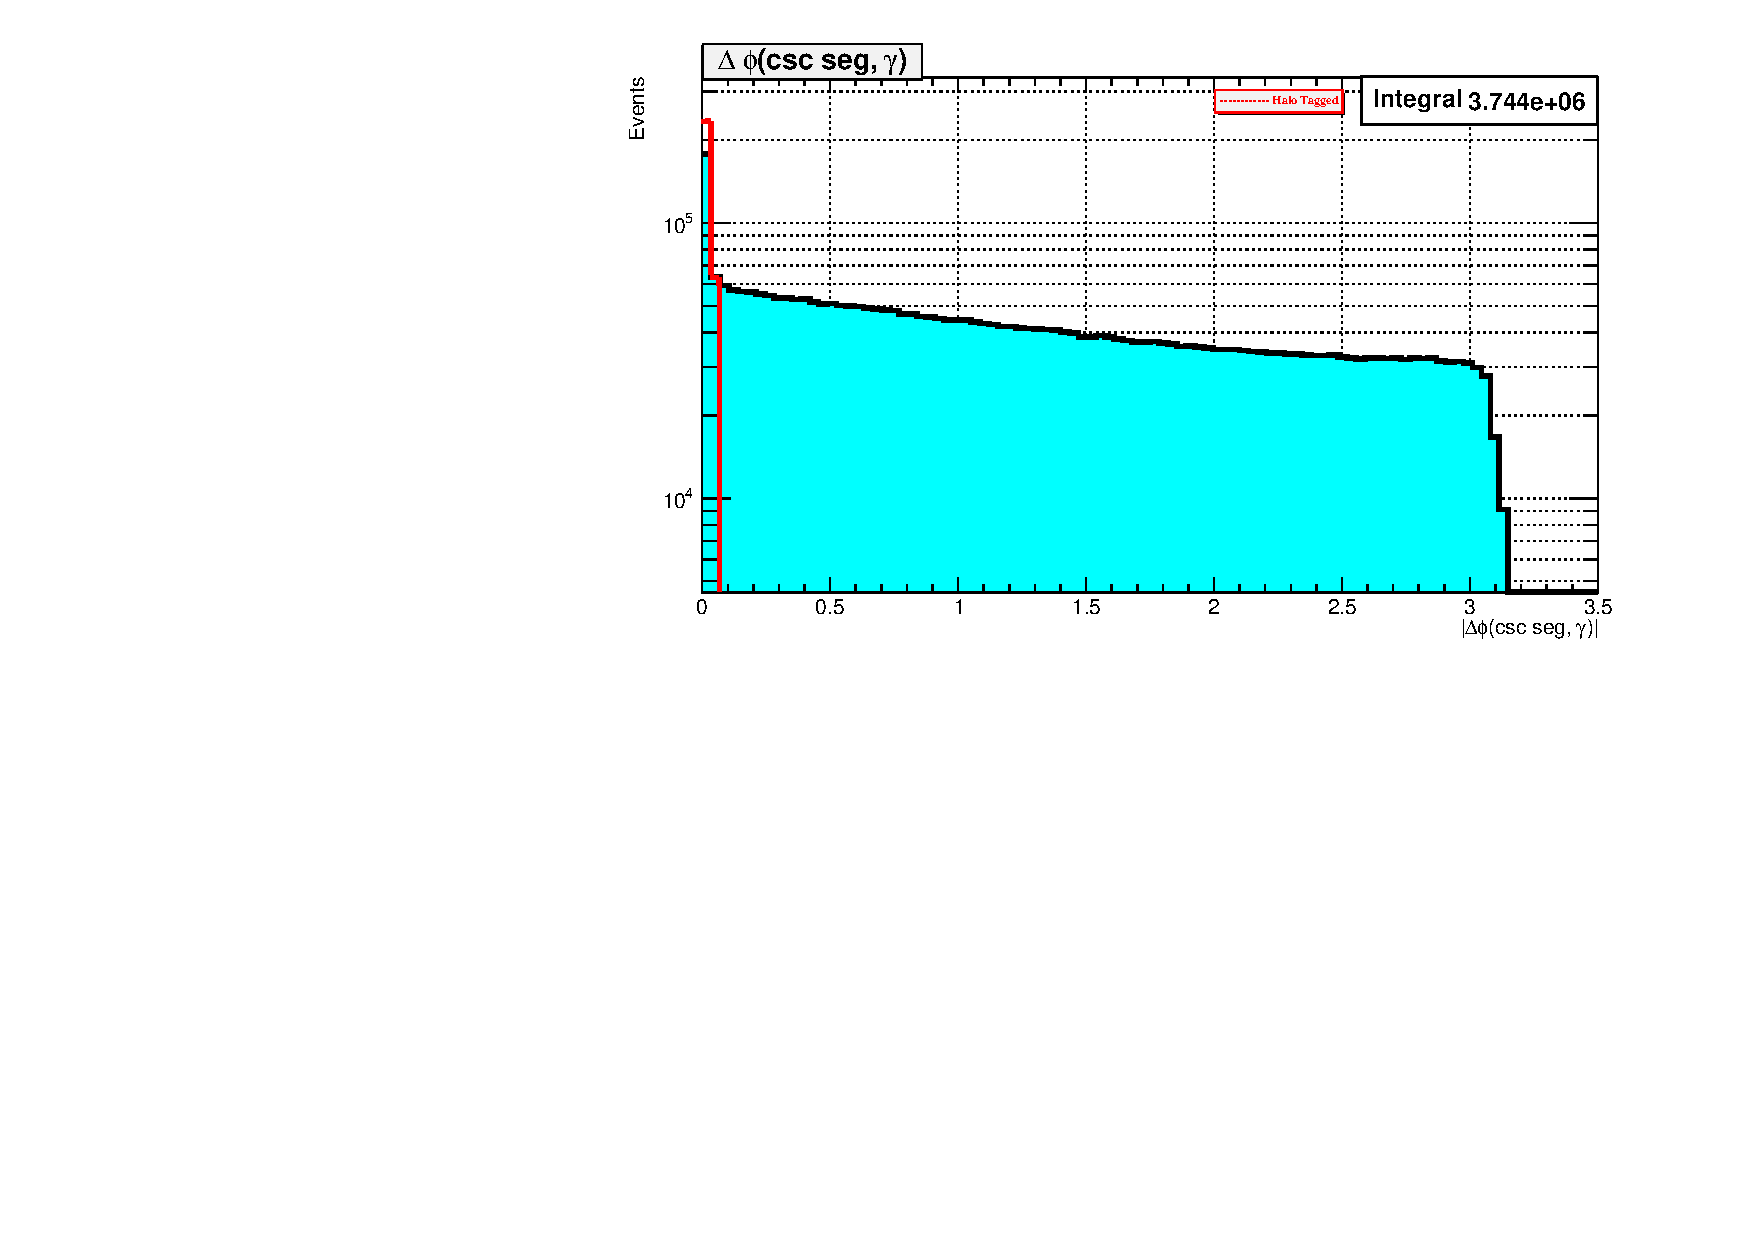
\includegraphics[height=6cm, width=0.5\textwidth]{THESISPLOTS/CSC-Segment-Halo-Tagging.pdf}
%{THESISPLOTS/CSC_Segment_Halo_data.png}
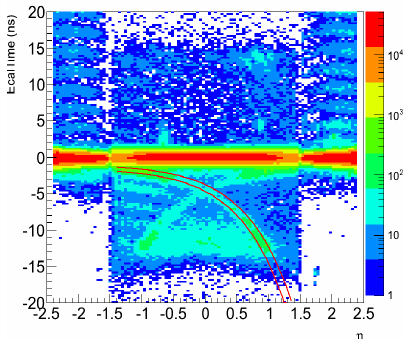
\includegraphics[height=6cm, width=0.5\textwidth]{THESISPLOTS/HALO-ECAL-TIME-Vs-ETA.png}}
\captionof{figure}{ECAL time Vs $\eta$~(left) and ECAL time Vs $\phi$~(right) and $CSC(Seg,\gamma)\Delta\phi$  for photons with $\pt > 80$~GeV from data. Halo photons show a clear matched between CSC segments and ECAL cluster in $\Delta\phi$  with their distribution peaking at $\phi = 0, \pm \pi$ and also the shape of their expected time.}
\label{fig:HALO}
\end{center} 



\subsubsection{Cosmic-Ray Photons}
Cosmic muons like beam Halo muons produced with sufficient energy  will bremsstrahlung in the ECAL producing photons referred here as \textit{cosmic-ray photons}. Unlike halo muons, cosmic muons can arrive at ECAL from any direction. Nevertheless, they are expected to hits in the Drift Tubes~(DT) segments. Thus, using the DT and corresponding  muon photon clusters in ECAL we can match the  hit position in DT segments to ECAL clusters within $\Delta\eta$ and $\Delta\phi$ between the DT segment hit and the ECAL cluster. The two dimensional distribution for $DT\Delta\eta(DT,\gamma)$ and $DT\Delta\phi(DT,\gamma)$ shown in figure \ref{fig:COSMIC} is shown for events with photon time above $2$~ns and time below $-3$~ns. Events containing photons with small $\Delta\eta$ and $\Delta\phi$ are considered to be strong candidates for cosmic-ray photons. The same variables is used to identify cosmic-ray photons from a pure cosmic ray(data taken when there are no proton-proton collisions) sample and the distributions show very similar features as can be seen in figure 
\ref{fig:COSMIC}.

\begin{center}
\centering
\mbox{
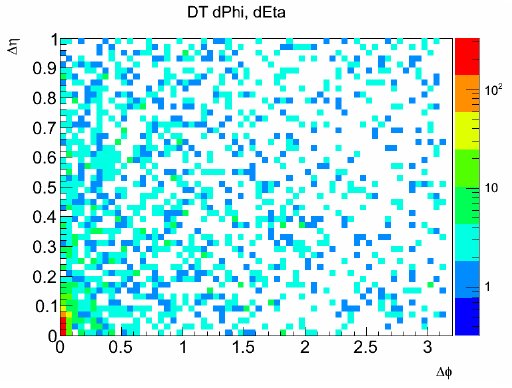
\includegraphics[height=6cm, width=0.5\textwidth]{THESISPLOTS/Cosmic_Ray_Photons_Data.png}
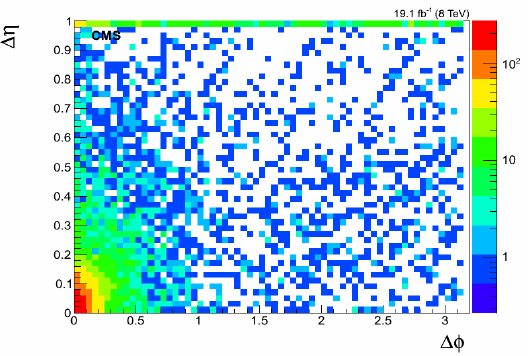
\includegraphics[height=6cm, width=0.5\textwidth]{THESISPLOTS/Cosmic_Ray_Photons_Cosmic_dataset.png} }
\captionof{figure}{Two dimensional plot showing $DT\Delta\phi(Seg,\gamma)$ against $DT\Delta\eta(Seg,\gamma)$ for photons with $\pt > 80$~GeV, ECAL Time $> 2$~ns and ECAL Time $< -3$~ns in proton-proton collision data~(left) and non-proton-proton collision or cosmic data~(right). Small $\Delta\eta$ and $\Delta\phi$ are cosmic-ray photon candidates.}
\label{fig:COSMIC}
\end{center}

\subsubsection{Anomalous Photons: Spikes}
Neutrons and some charge hadrons depositing their energy directly to the APDs instead of the crystal scintillation are referred to as \textit{anomalous signal} or \textit{spikes}. These spikes can mimic true photons from proton-proton collisions  leading to mis-identification of spikes as photons. Spikes are easily miss-identified as energetic photons and isolated. However, most spikes show a different signal pulse shape to that of photons and also have large negative ECAL time. In addition to energy topological selection cuts and ECAL cleaning that is done during online and offline event selection, ECAL clusters belonging to spikes are usually made up of very few crystals compared to photons clusters with many crystals. Thus using the number of crystals making in a reconstructed super cluster, we can distinguish true isolated photons from events with spikes. It has been observed that spike contributions increases with increase in LHC luminosity. Thus, as a selection criteria, photons with  Not identified as cosmic-ray photons or halo photons and with number of good crystals less than $7$ are considered to be spike candidates. Figure \ref{fig:SPIKES} show the distribution of the number crystals in a photon super cluster comparing photons with ECAL time $ < 0$~ns, some in-time photons~( ECAL $ -2 < t < 0$~ns and  selected spike and halo control sample. The spike control sample is selected using the "swiss-cross" variable which is used to identify and reject events with spikes during super cluster reconstruction. We observe that most spikes always have fewer($ < 7$) crystals contributing to the photon super cluster.

\begin{center}
\centering
\mbox{
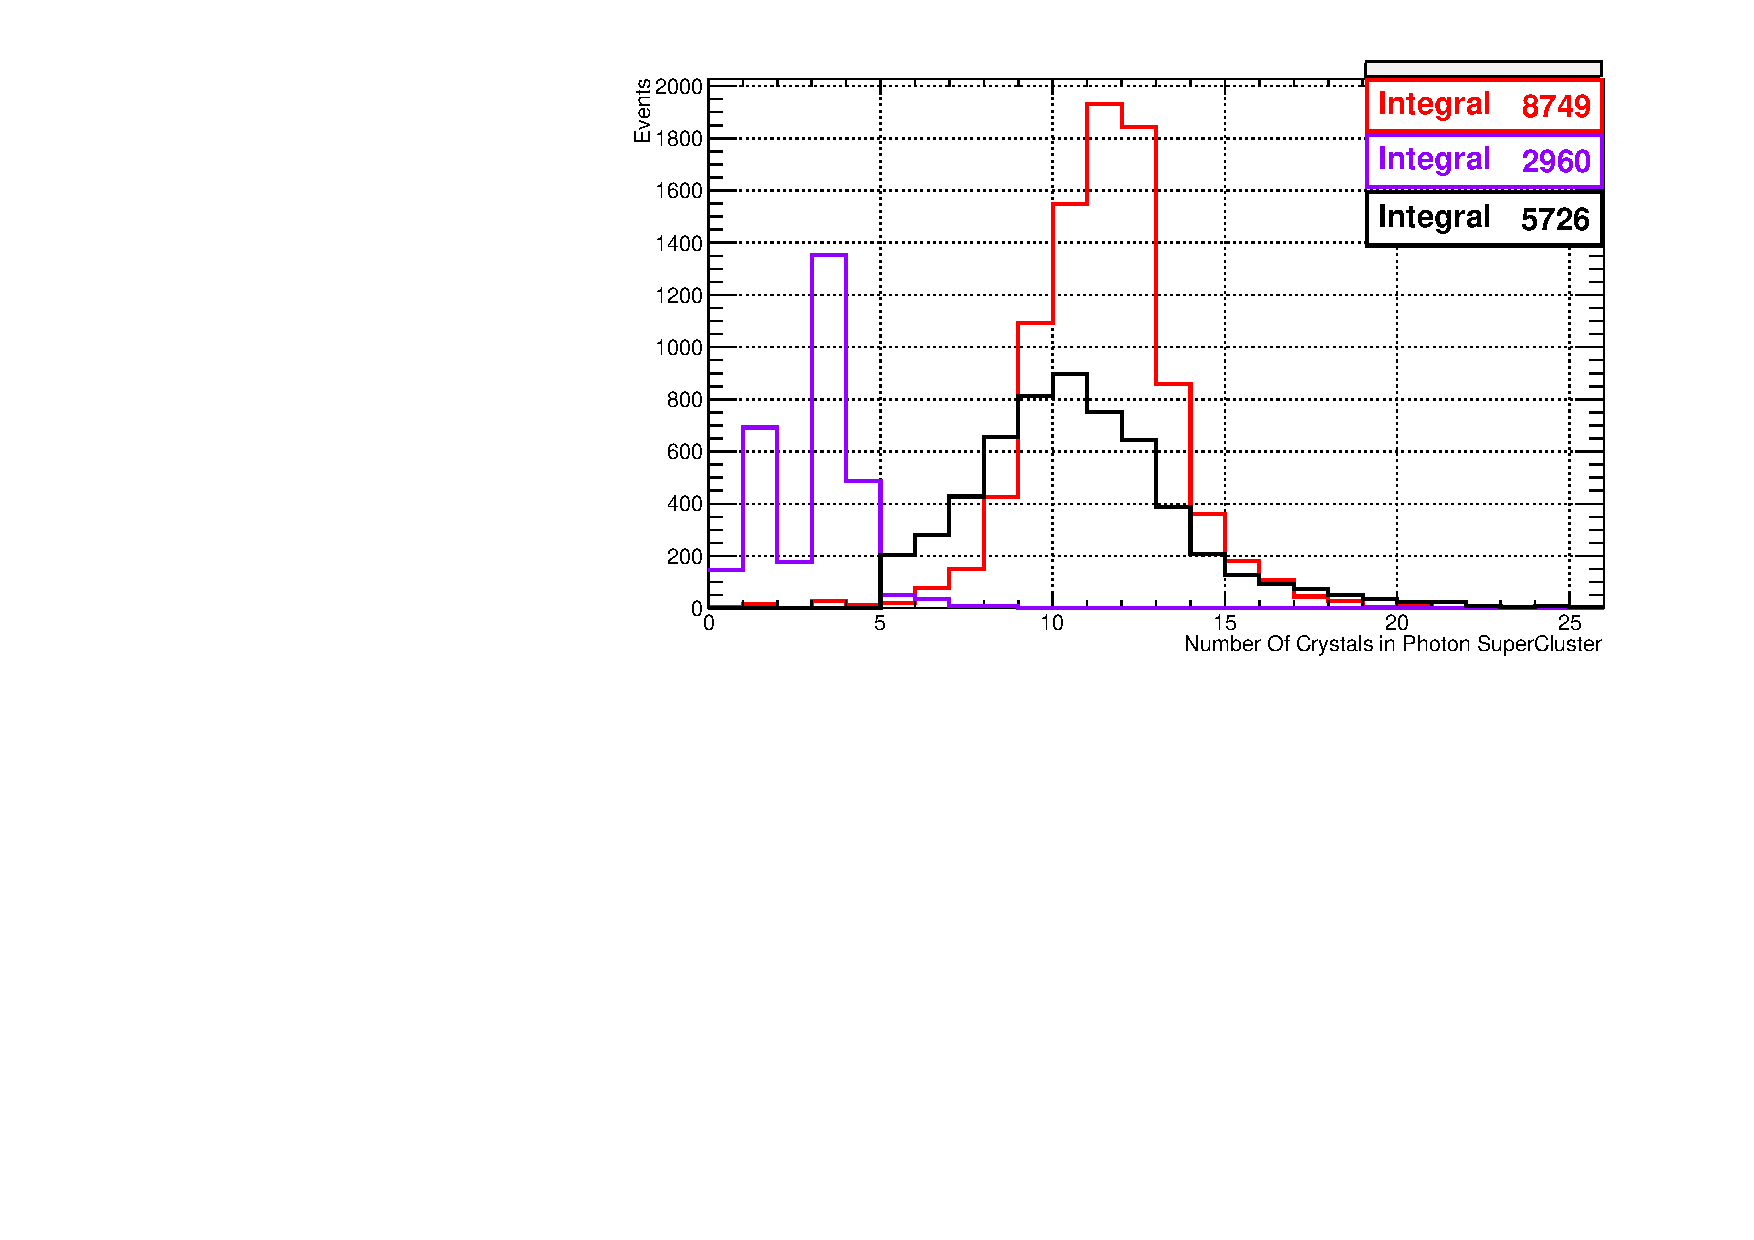
\includegraphics[height=7cm, width=0.7\textwidth]{THESISPLOTS/Number-Of-Crystals-In-Photon-SC.pdf}}
%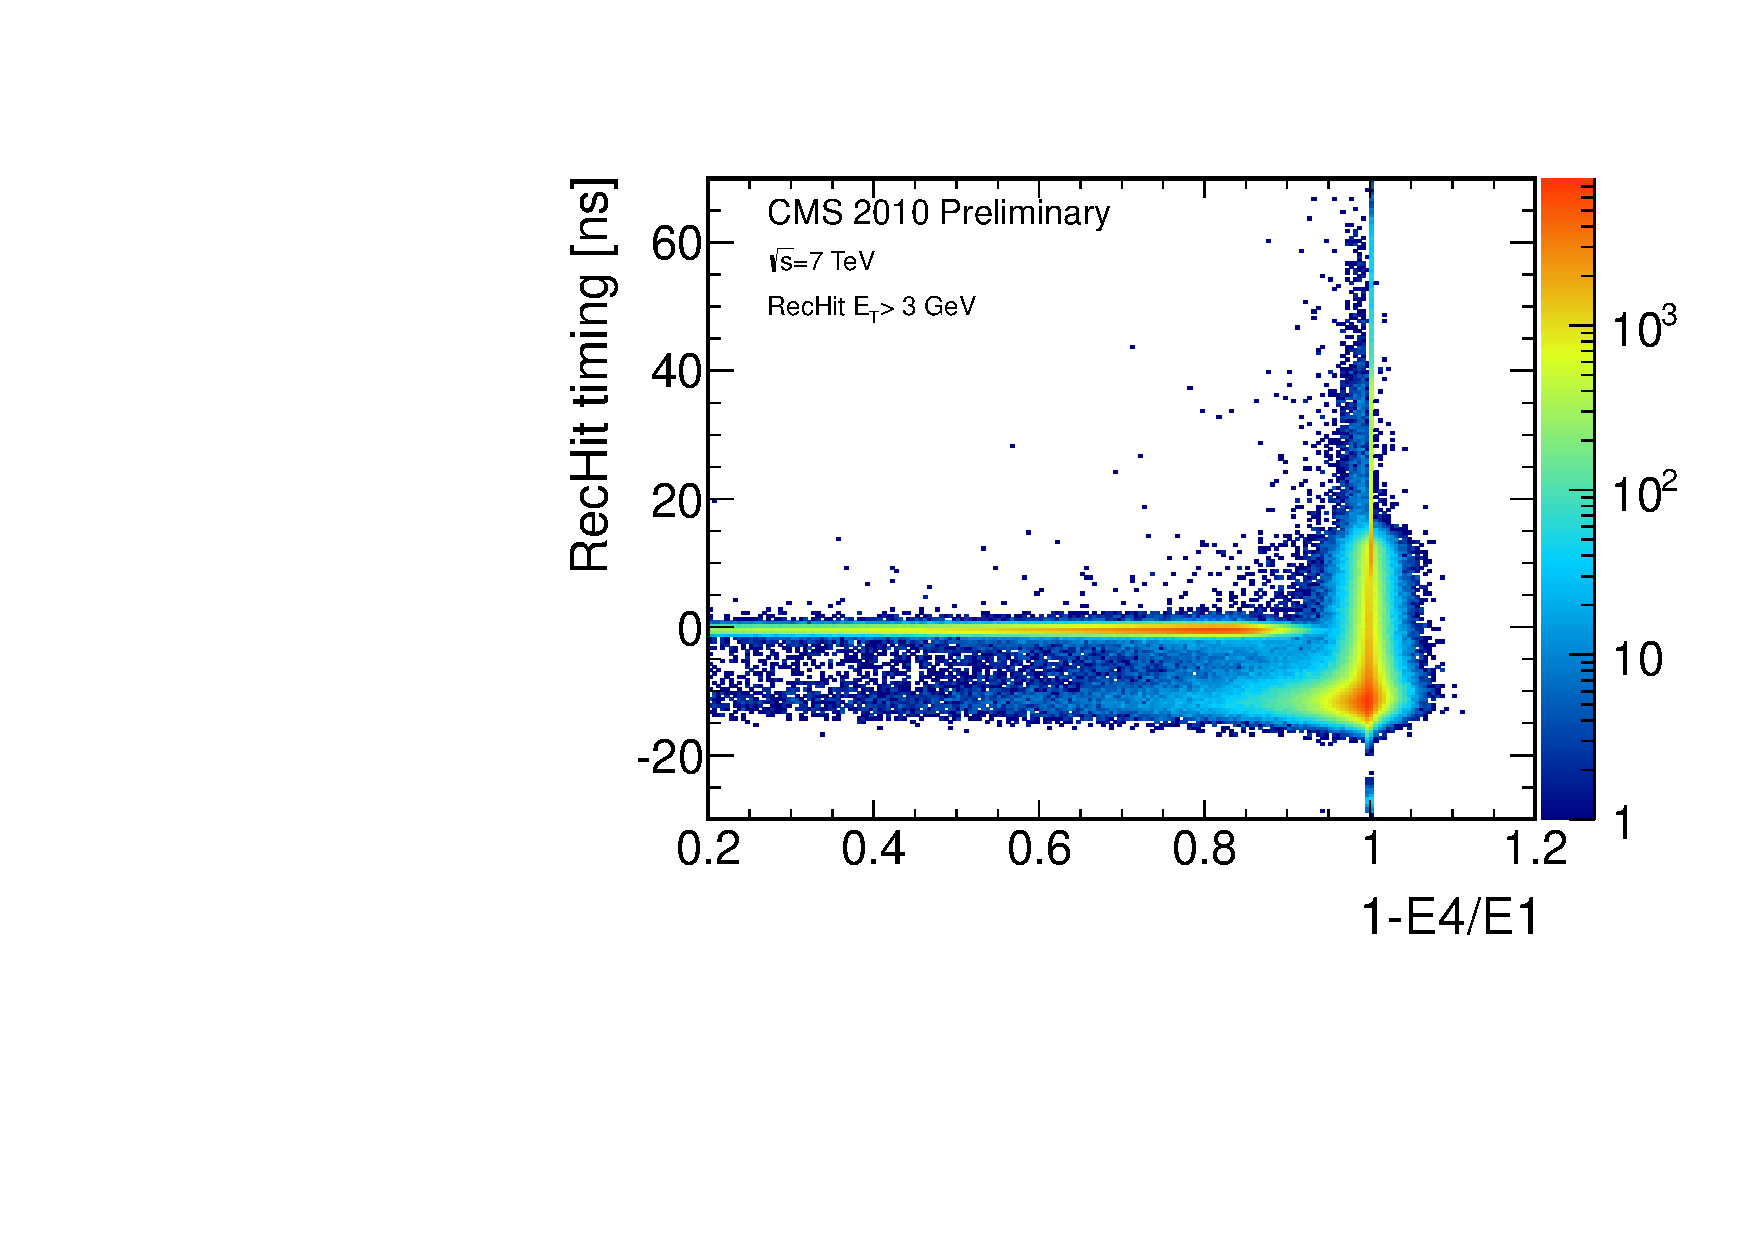
\includegraphics[height=7cm, width=0.5\textwidth]{THESISPLOTS/swisscross_vs_time_3GeV.pdf} }
\captionof{figure}{Plot showing  Number of crystals in photon super cluster for photons from the region with ECAL Time $ < 0$~ns. We define control regions of candidate photons(black), spike candidate photons~(magenta) and halo candidate photons~(red).}
\label{fig:SPIKES}
\end{center}


\subsection{Collision Backgrounds}

\subsubsection{QCD Photons and Pile Up}
The LHC provides proton-proton collisions every $25$~ns, however during the \texttt{2012 LHC} run, these bunch spacing time increased to $50$~ns. However, as discussed in section $3.1.5$ on LHC Bunch structure, the presence of 
Satellite/ghost bunches spaced in $5.0$~ns or $2.5$~ns  can also contribute to producing delayed photons either from collisions between these satellite/ghost bunches or with the main proton bunch collisions.
As observed in figure \ref{fig:TIMEECAL}, photons from these events are a serious background source to delayed photons and most of these photons will pass all the above event and photon criteria selections. Thus, a careful 
estimation of this contribution is the major task of the background estimation in this analysis.
The kinematics of these events are very similar and as a result, we employ the standard \texttt{ABCD} method to for estimating these background contribution  to the signal region.

Before proceeding, we should mention another possible concern which deals with the difference in the measurement of \MET in most analysis which mostly require events to be \textit{in-time} to this
analysis whose event selection has been extended to include \textit{Out-of-time} events.

\paragraph*{\MET Re-Calculation}\mbox{}\\
The presence of timing cuts of $|t_{RECO}| > 3.0$~ns in EB in the official CMS electromagnetic super cluster reconstruction as an "out-of-time" event cleaning procedure, results in a difference in the calculation of \MET for "in-time" events~($|t_{\gamma}| < 3.0$~ns) and "out-of-time" events~($|t_{\gamma}| > 3.0$~ns). Out-of-time photons are not taking into consideration when calculating the total transverse momentum of an event to derived the total transverse momentum imbalance, thus, we have to recalculate the \MET for events with out-of-time photons taking into consideration \pt contributions from these out-of-time photon. This results in us using two different sets of \MET whose   definition are given as follows:
\begin{enumerate}
\item ${\MET}_{1}$: \MET for events where photon \pt contributions is not included during \MET measurements.
\item ${\MET}_{2}$: \MET of the event taking into account out-of-time photon \pt contributions in \MET measurements.
\end{enumerate}
  
The distributions for ${\MET}_{1}$ and ${\MET}_{2}$  against ECAL time can be seen in figure \ref{fig:METS}.

\begin{center}
\centering
%\mbox{
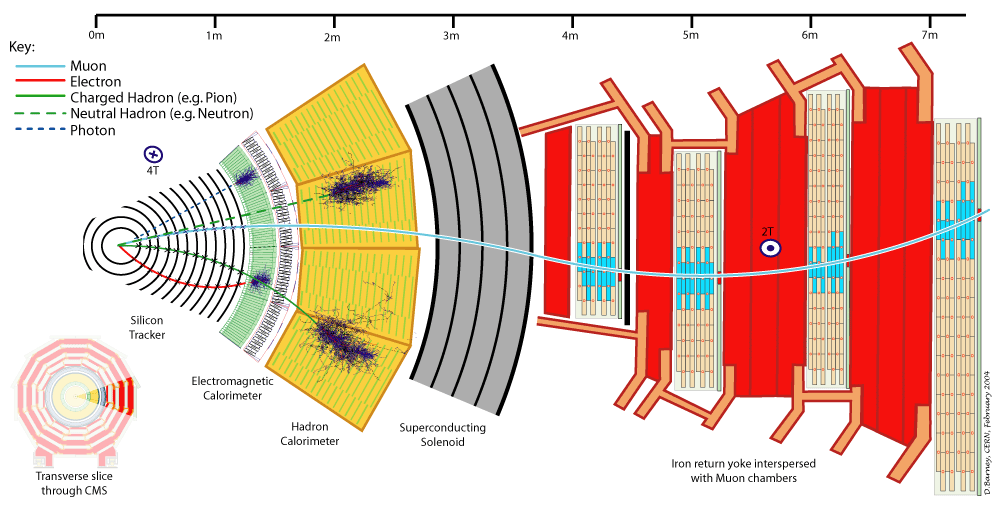
\includegraphics[scale=0.2]{THESISPLOTS/CMS_Slice.png}
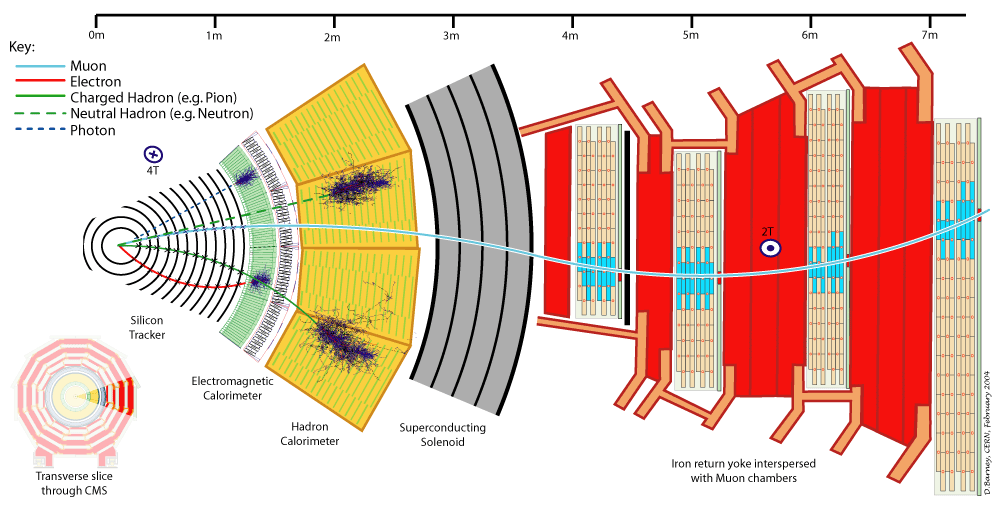
\includegraphics[scale=0.2]{THESISPLOTS/CMS_Slice.png}
\captionof{figure}{Figure showing \MET distributions for events with out-of-time and in-time photons. ${\MET}_{1}$ and ${\MET}_{2}$ definitions are given in context. }
\label{fig:METS}
\end{center}

\subsection{Event Cleaning}
Using the above observables for studying halo, cosmic and spike photons we reduced the contribution of these events by applying in addition to our above selections the following selections:
\begin{itemize}
\item Veto 0-jet events as this sample is highly populated with beam halo events, 
\item Veto events with $CSC(Seg,\gamma)\Delta\phi < 0.05$,
\item Only photons with $|\eta_{\gamma}| < 1.45$ are considered,
\item Photons must have Number of Good crystals $ > 7$,
\item Photons tagged as halo and cosmic are removed,
\item Event must have at least 1-jet.
\end{itemize}
Events which pass all these additional selection criteria make up the sample which is used to estimated the background to our signal.

\paragraph*{•} 
\par
In order to estimating the background contribution from collision and non-collision sources, we employ a 3-dimensional space involving ${\MET}_{1}$, ${\MET}_{2}$ and ECAL time.  Our signal region is events with $t > 3.0$~ns and large \MET where by large \MET we mean events with  large  ${\MET}_{1}$ and  ${\MET}_{2}$. Non-collision events have large time as they are mostly out-of-time and by \MET calculation requirements should have large  ${\MET}_{2}$. While collision produced backgrounds events are mostly in-time and may often be measured with $t > 3.0$~ns due to either mis-reconstruction or from ghost/satellite contributions. However, these events cannot be produced with large correctly calculated \MET because for example in $\gamma +$ jets events, very small \MET due to energy miss-measurements is expected to be produced.
 But if the collision event is produced and arrives at ECAL with $t > 3$~ns, and the \MET is not properly calculated (since events with photons ECAL time, $|t| > 3$~ns are rejected during standard super cluster reconstruction with their \pt contribution  not taken into account in the \MET calculation) which in this case is large ${\MET}_{1}$, they will fluctuate or be easily considered as additional contribution to the non-collision background estimation in our signal region.
Therefore, we select samples or control regions~(CR) which enhances each interested background source and use that CR to estimate the enhanced background contribution taking into account the possible contamination of an alternate background source due to possible fluctuations in event rate.
The overall estimation technique is verified through a closure test procedure and the collision background estimation verified and validated using an extra control sample of $Z \rightarrow \ell \ell$ events where the $\ell$ are electron candidates reconstructed using photon candidates extended to include out-of-time events.

Signal Region: Events with ${\MET}_{2} > 60$~GeV, ${\MET}_{1} > 60$~GeV and $t > 3.0$~ns.
\paragraph*{${\MET}_{2} > 60$~GeV } : CR in which collision~(QCD) background is suppressed while that for halo, cosmic ray and spike photon are all enhanced.
Within this space, we define four regions representing ABCD to estimate the the background contribution:
\begin{itemize}
\item A: Events with ${\MET}_{1} < 60$~GeV and $t < -3.0$~ns.
\item C: Events with ${\MET}_{1} < 60$~GeV and $t >  3.0$~ns.
\item B: events with ${\MET}_{1} > 60$~GeV and $t < -3.0$~ns.
\item D: events with ${\MET}_{1} > 60$~GeV and $t >  3.0$~ns.
\end{itemize}
Thus, the number of events expected in CR D under the assumption that $\frac{N_{D}}{N_{B}} = \frac{N_{C}}{N_{A}}$  is given as:

\begin{equation}
N_{D} = \left(\frac{N_{B}}{N_{A}} \right)\cdot N_{C}
\end{equation}

\paragraph*{${\MET}_{1} > 60$~GeV }: CR in which non-collision background~(halo, cosmic and spike photons) contribution is suppressed wheras collision~(QCD) background contribution is enhanced.
Further dividing this CR into according to $A^{\prime}$,$B^{\prime}$,$C^{\prime}$,$D^{\prime}$ to estimate its contribution where:
\begin{itemize}
\item $A^{\prime}$: Events with ${\MET}_{2} < 60$~GeV and $t < -3.0$~ns.
\item $B^{\prime}$: Events with ${\MET}_{2} > 60$~GeV and $t < -3.0$~ns.
\item $I^{\prime}$: Events with ${\MET}_{2} < 60$~GeV and $|t| < 2.0$~ns.
\item $I$: Events with ${\MET}_{2} > 60$~GeV and $|t| < 2.0$~ns.
\end{itemize}
we also define a in time CR as:
\begin{itemize}
\item $C^{\prime}$: Events with ${\MET}_{2} < 60$~GeV and $t >  3.0$~ns.
 \item $D^{\prime}$: Events with ${\MET}_{2} > 60$~GeV and $t >  3.0$~ns.
 \item $I^{\prime}$: Events with ${\MET}_{2} < 60$~GeV and $|t| < 2.0$~ns.
\item $I$: Events with ${\MET}_{2} > 60$~GeV and $|t| < 2.0$~ns.
\end{itemize}

Now using using the above regions we can estimate the contributions of collision background in both CRs $B$ and $D$ as follows:
\begin{equation}
\displaystyle{N^{B}_{col} = N_{B^{\prime}}  = \left( \frac{I}{I^{\prime}} \right)\cdot N_{A^{\prime}}}, \quad \quad
\displaystyle{N^{D}_{col} = N_{D^{\prime}}  = \left( \frac{I}{I^{\prime}} \right)\cdot N_{C^{\prime}}}
\end{equation}
where we have assumed that $\frac{N_{B^{\prime}}}{N_{A^{\prime}}}  = \frac{N_{I}}{N_{I^{\prime}}}$ and  $\frac{N_{D^{\prime}}}{N_{C^{\prime}}}  = \frac{N_{I}}{N_{I^{\prime}}}$.
\newline

$N^{B}_{\mbox{col}}$ and $N^{D}_{\mbox{col}}$ are collision contributions to  CRs $B$ and $A$ such that the final non-collision background estimation~(since the dominant contribution to total background  is the non-collision background source) is given as:

\begin{equation}
N^{D}_{\mbox{Total}} = \left(\frac{N_{B} - N^{B}_{col} }{N_{A}} \right)\cdot N_{C} + N^{D}_{\mbox{col}} 
\end{equation}\label{eq:bkg}
where $N^{D}_{\mbox{Total}} = N^{D}_{\mbox{non-col}} + N^{D}_{\mbox{col}}$ is the total background estimation in  our signal region.
A diagram showing the above background estimation technique is shown in figure \ref{fig:BKGESTI}.
\begin{center}
\centering
%\mbox{
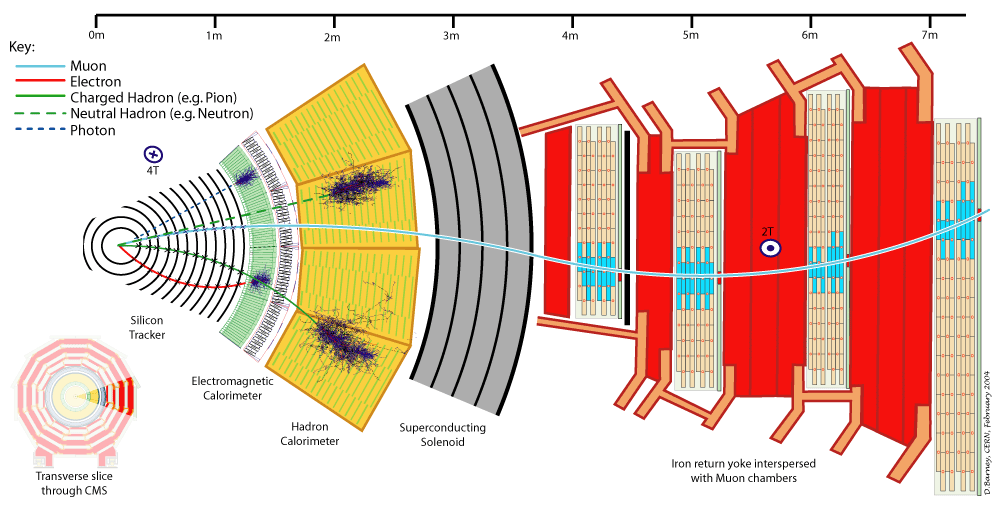
\includegraphics[scale=0.2]{THESISPLOTS/CMS_Slice.png}
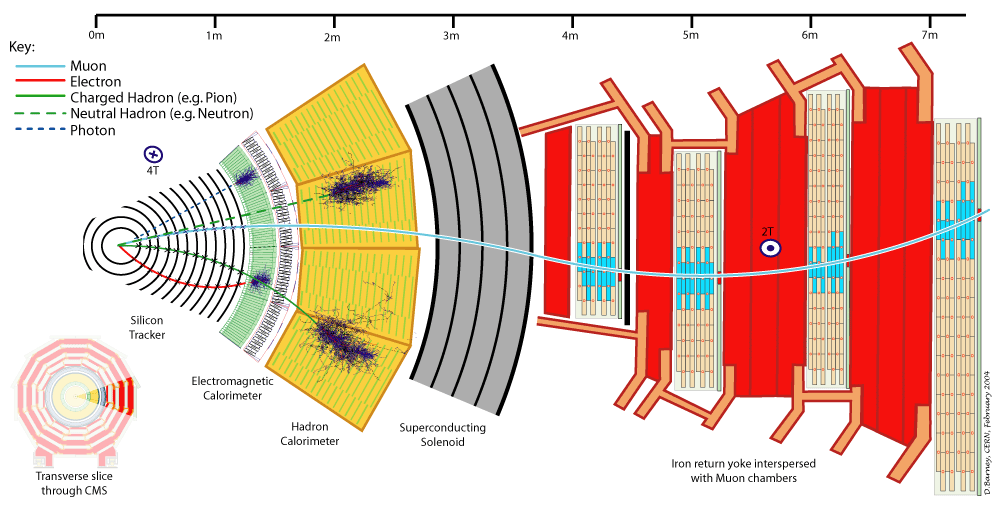
\includegraphics[scale=0.2]{THESISPLOTS/CMS_Slice.png}
\captionof{figure}{Diagrams showing background estimation technique.}
\label{fig:BKGESTI}
\end{center}

A closure test using events with $0-\mbox{jets}$ and $1-jet$ is used to verify the above  background estimation technique and the above assumptions are cross checked using $Z\rightarrow e^{+} e^{-}$ events. 
The underlying assumption here is that background contributions to large timing from collision source referred here as QCD is very small and must be of the order of $10^{-5}$ in comparison to in-time photons. i.e the ratio 
$ N_{t > 3~ns}/ N_{|t| < 2.0~ns} \approx 10^{-5}$ with $N$ being the number of photons.

\paragraph*{Closure Test}\mbox{}\\
By selecting a sample of events containing only a single jet, we verify the validity of our method of background estimation using a closure test. The closure test is simply comparing the number of events we observed in our signal region \texttt{D} with the number we expect from using our \texttt{ABDC} background estimation method.
Using a equation \ref{eq:bkg}, we observed a total of $5$-events when we expected $6.44^{+2.95}_{-3.45}$ which is quite close. This gives us confidence that our  background estimation method is robust and reliable and we can now move on to do our final background estimation on dataset with events having at least $2$-jets passing our final photon, jet and \MET selection after being cleaned.
\subsection{Background Estimation Cross Check}
The main assumption in our background estimation technique is that, the contribution from collision background events to our signal region~($|time| > 3$~ns) is negligible.
In order to show this we select $Z\rightarrow e^{+} e^{-}$ events from \texttt{SingleElectron/} and \texttt{DoubleElectron/} data sets of 2012.
The selection criteria of our extended to include out-of-time $Z$ candidates events is as follows:
\begin{itemize}
\item The candidate two electrons for the $Z$ bosons must have individual $\pt > 20$~GeV,
\item The di-mass of these two electrons, $|m_{\ell_{1}, \ell_{2}} - 91| > 61$~$GeV/c^{2}$,
\item Each electron must be in the barrel, $|\eta_{\ell_{1}}| < 1.479$ and $ |\eta_{\ell_{2}}| < 1.479$.
\end{itemize}
 At the electron super cluster level,  we used the seed crystal time adjusted accounting for the effects due to electron time of flight as the electron time, after the seed crystal has passed all the recommended crystals or rechit cleaning criteria recommended by the ECAP DPG such as \texttt{kWeird}, \texttt{kBad}, \texttt{kPoorCalib} used in rejecting crystals showing anomalous behavior like spikes, noisy, bad crystals and poorly calibrated crystals.
In this cross-check, we define our signal region as $Z$-candidate events with a well defined mass from both electrons i.e  $76 < |m_{\ell_{1}, \ell_{2}}| < 100$~$GeV/c^{2}$ while the Control sample consists of events which do not fall into the signal category.
A quick look at the similar plots to figure \ref{fig:HALO} of the electron candidates from the \texttt{Single/DoubleElectron} dataset compared to the \texttt{SinglePhoton} dataset as seen in figure \ref{fig:Elec} indicate that contribution from cosmic, halo and anomalous photon events is much reduced and thus makes the $Z$ boson candidate events sample a reliable sample to disentangle non-collision contributions and only study collision background contributions as initial objective.
\begin{center}
\centering
\mbox{
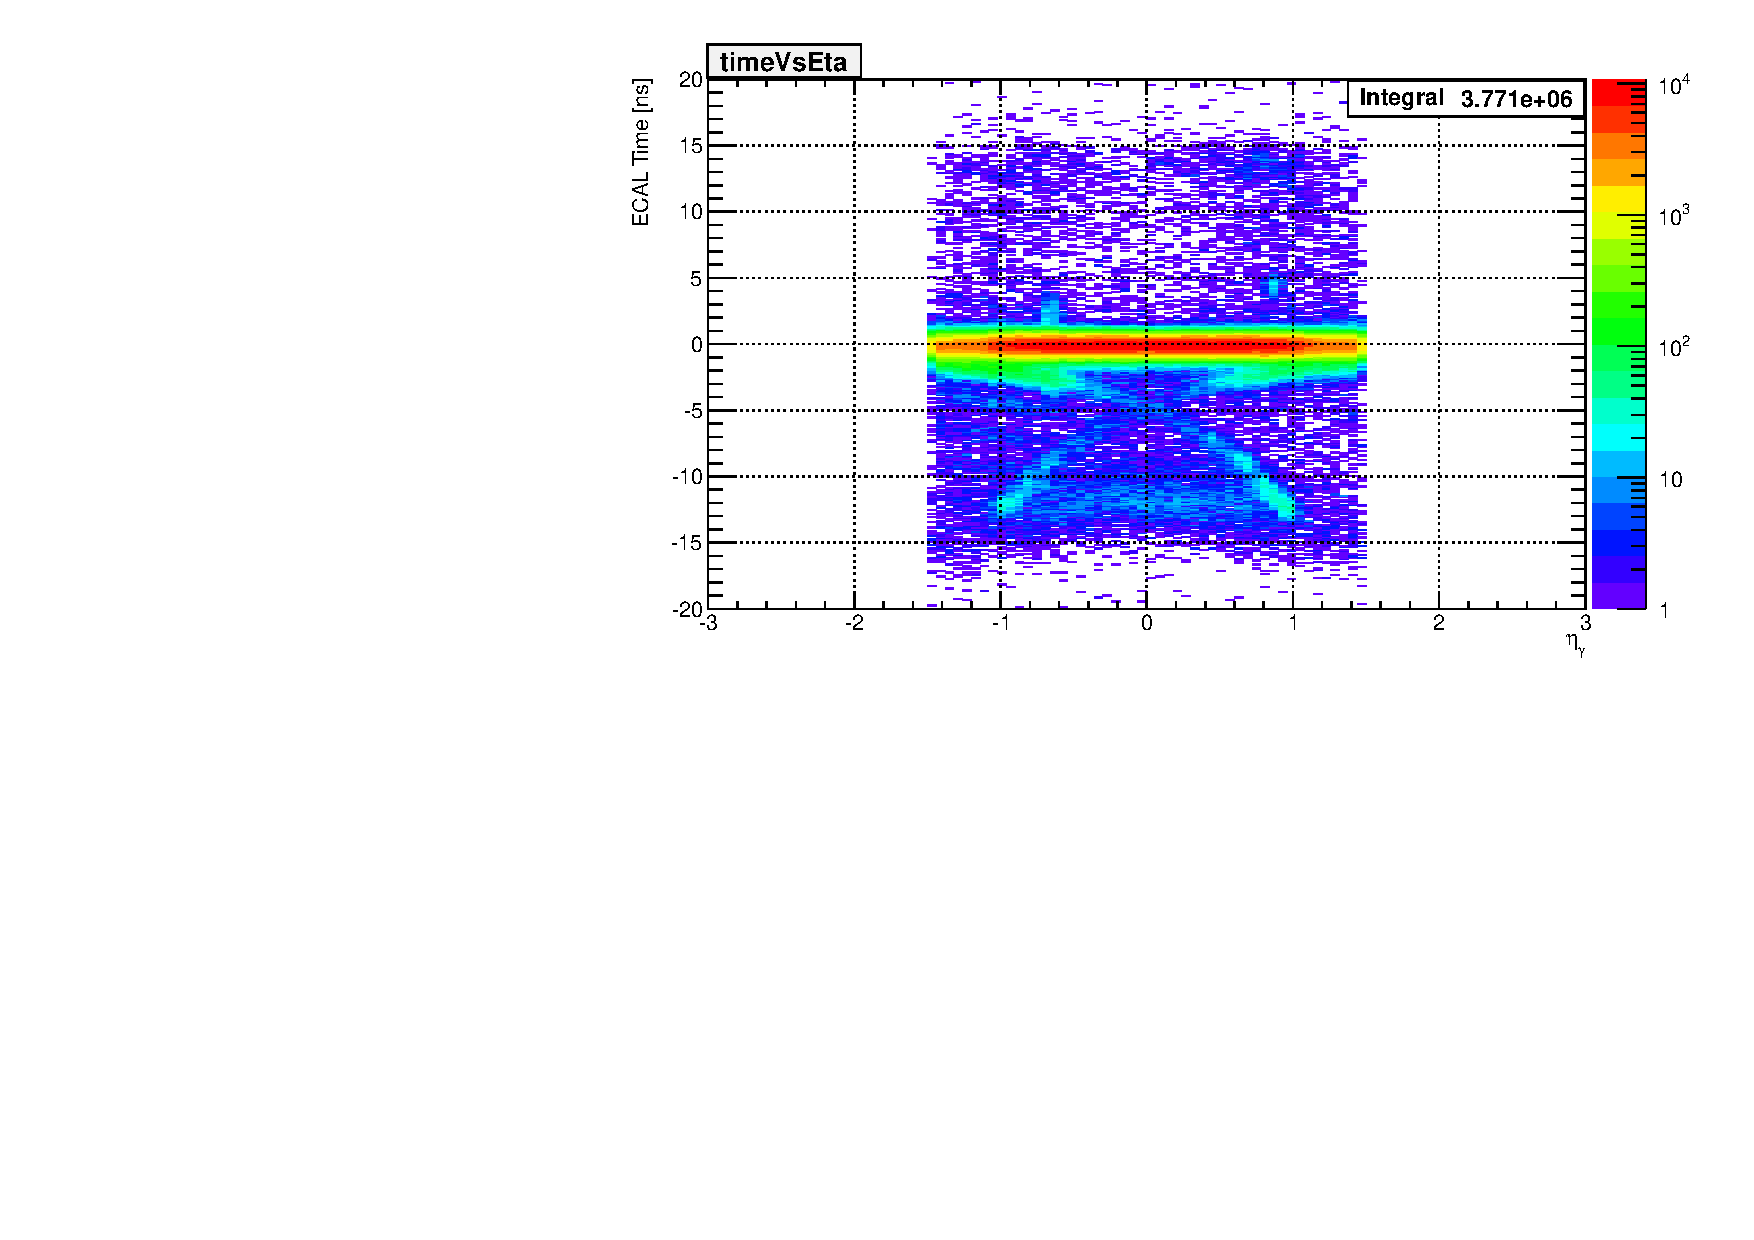
\includegraphics[height=7cm, width=0.5\textwidth]{THESISPLOTS/SinglePhotonDataSet-TimeVsEtaEB.pdf}
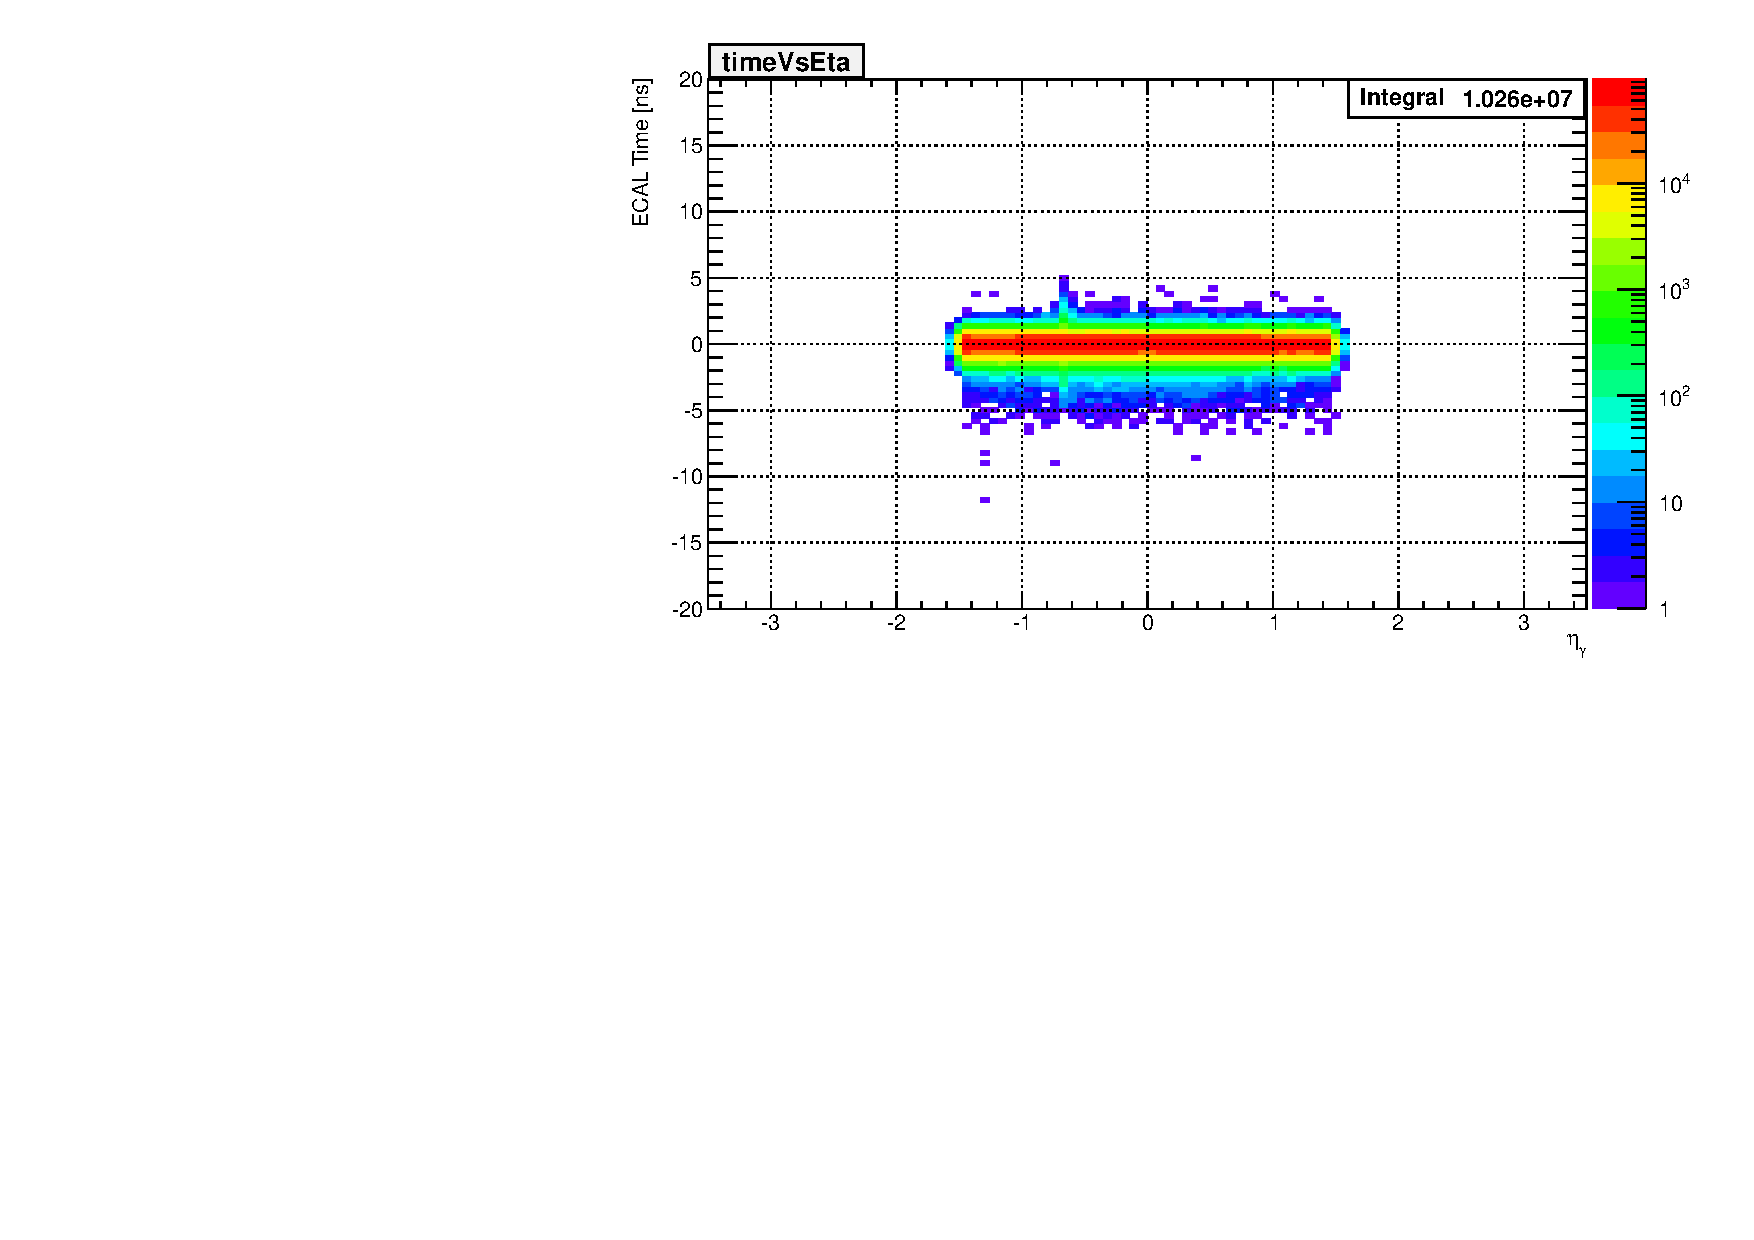
\includegraphics[height=7cm, width=0.5\textwidth]
{THESISPLOTS/ZCandidates_TimeVsEta.pdf}}
\mbox{
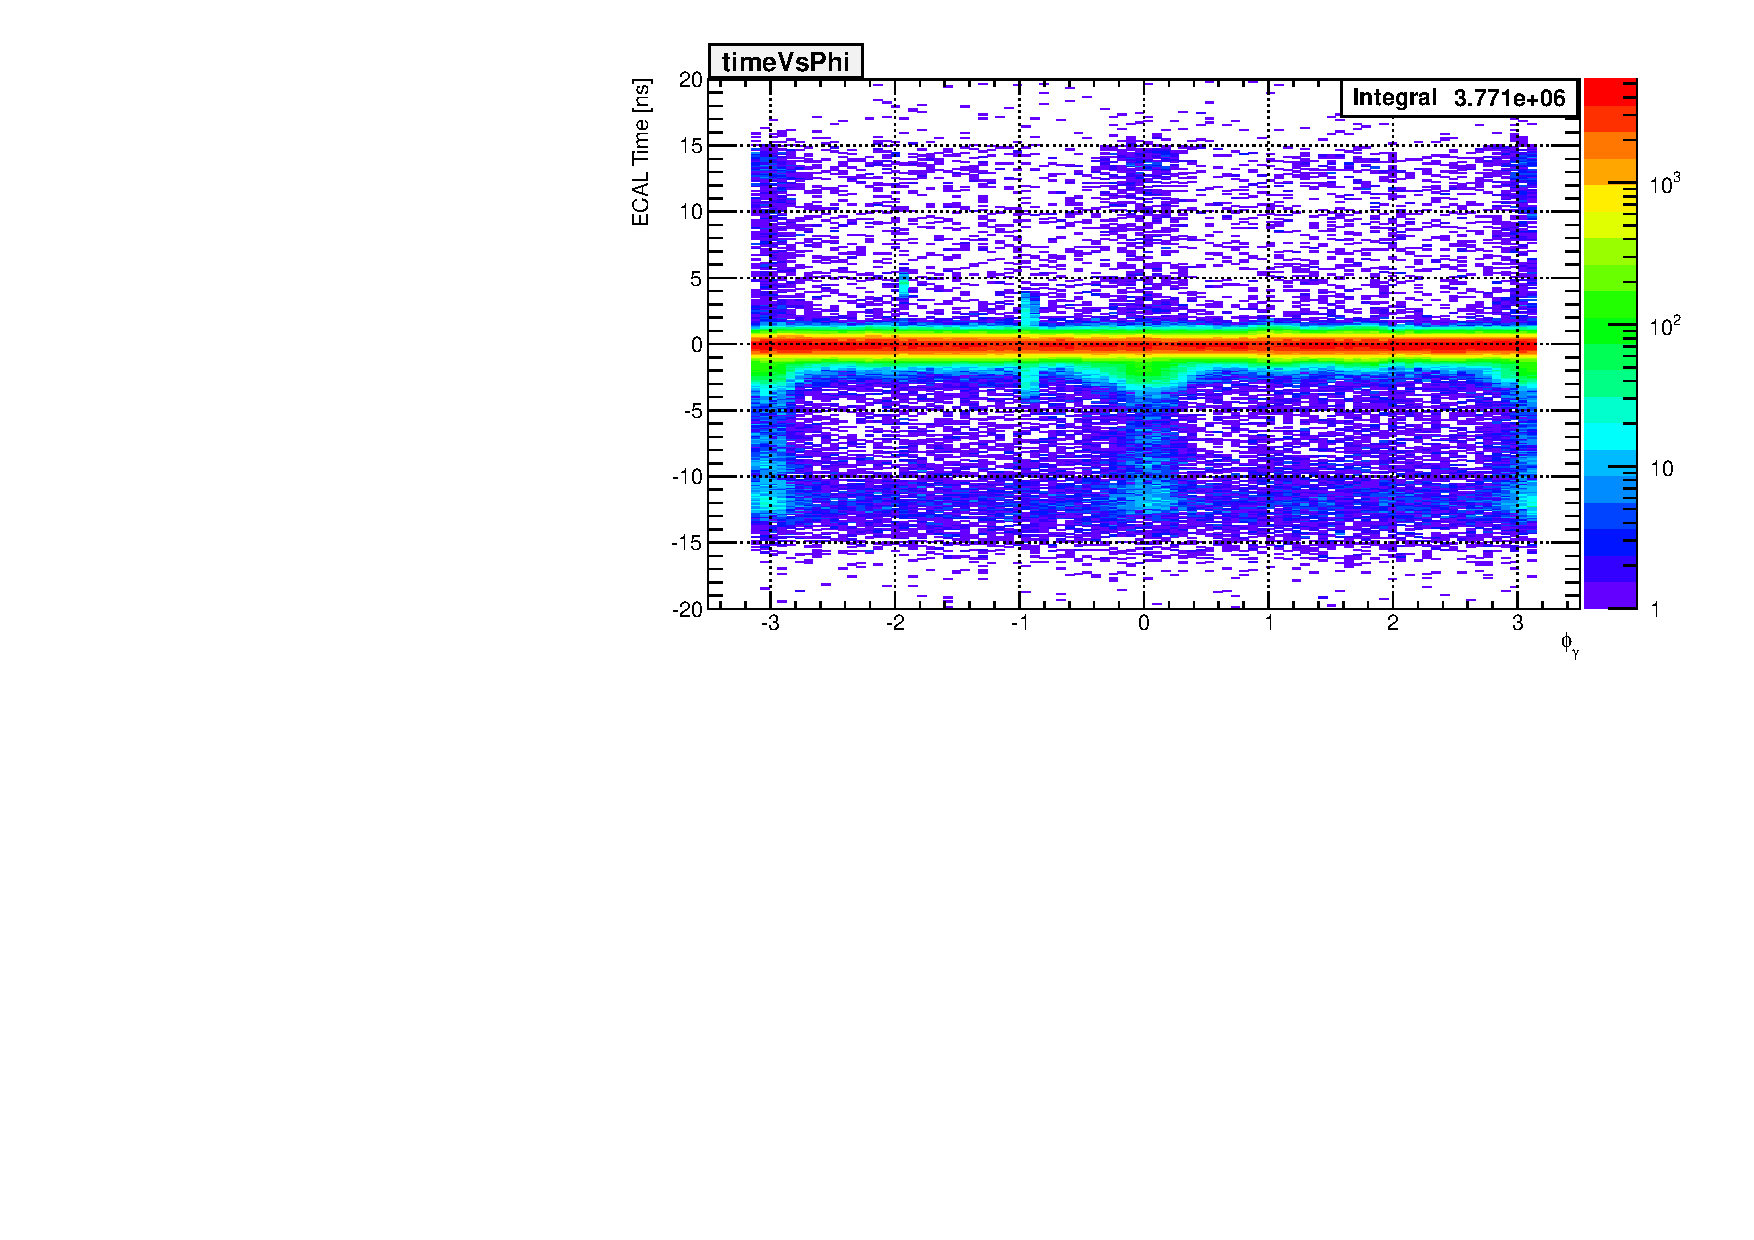
\includegraphics[height=7cm, width=0.5\textwidth]{THESISPLOTS/SinglePhotonDataSet-TimeVsPhiEB.pdf}
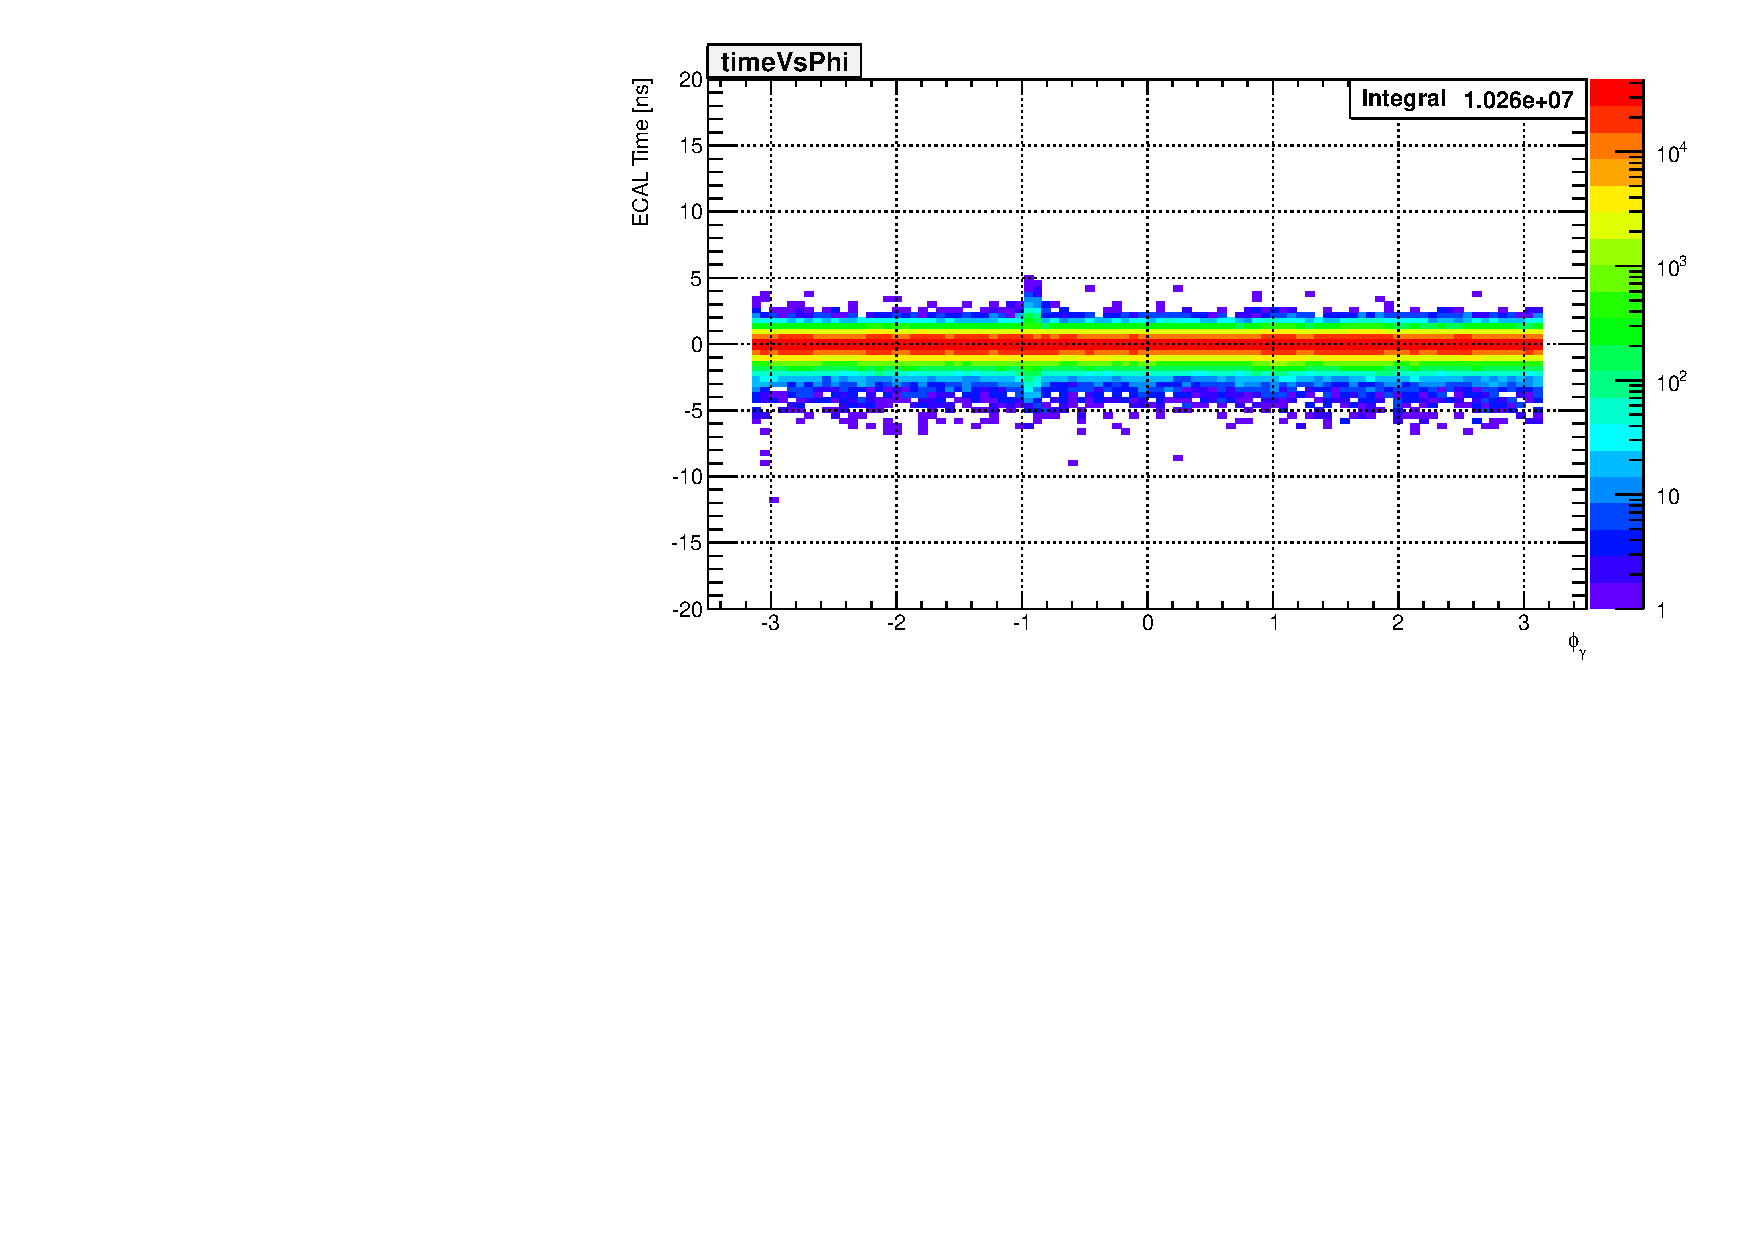
\includegraphics[height=7cm, width=0.5\textwidth]{THESISPLOTS/ZCandidates_TimeVsPhi.pdf}}
\captionof{figure}{ECAL time Vs $\eta$ and ECAL time Vs $\phi$~(left) for photons from \texttt{SinglePhoton} dataset~(left) compared with similar plots from the \texttt{DoubleElectron} dataset~(right). All photons are in barrel subdetector with $\phi = 0, \pm \pi$ mostly halo photons are not observed in the $Z$ boson candidate sample.}
\label{fig:Elec}
\end{center}

Figure \ref{fig:Zmass} shows the $Z$ boson mass reconstructed from the candidate electrons and timing of each electron for Signal~(left and blue) and for our control sample~(right and red).

\begin{center}
\centering
\mbox{
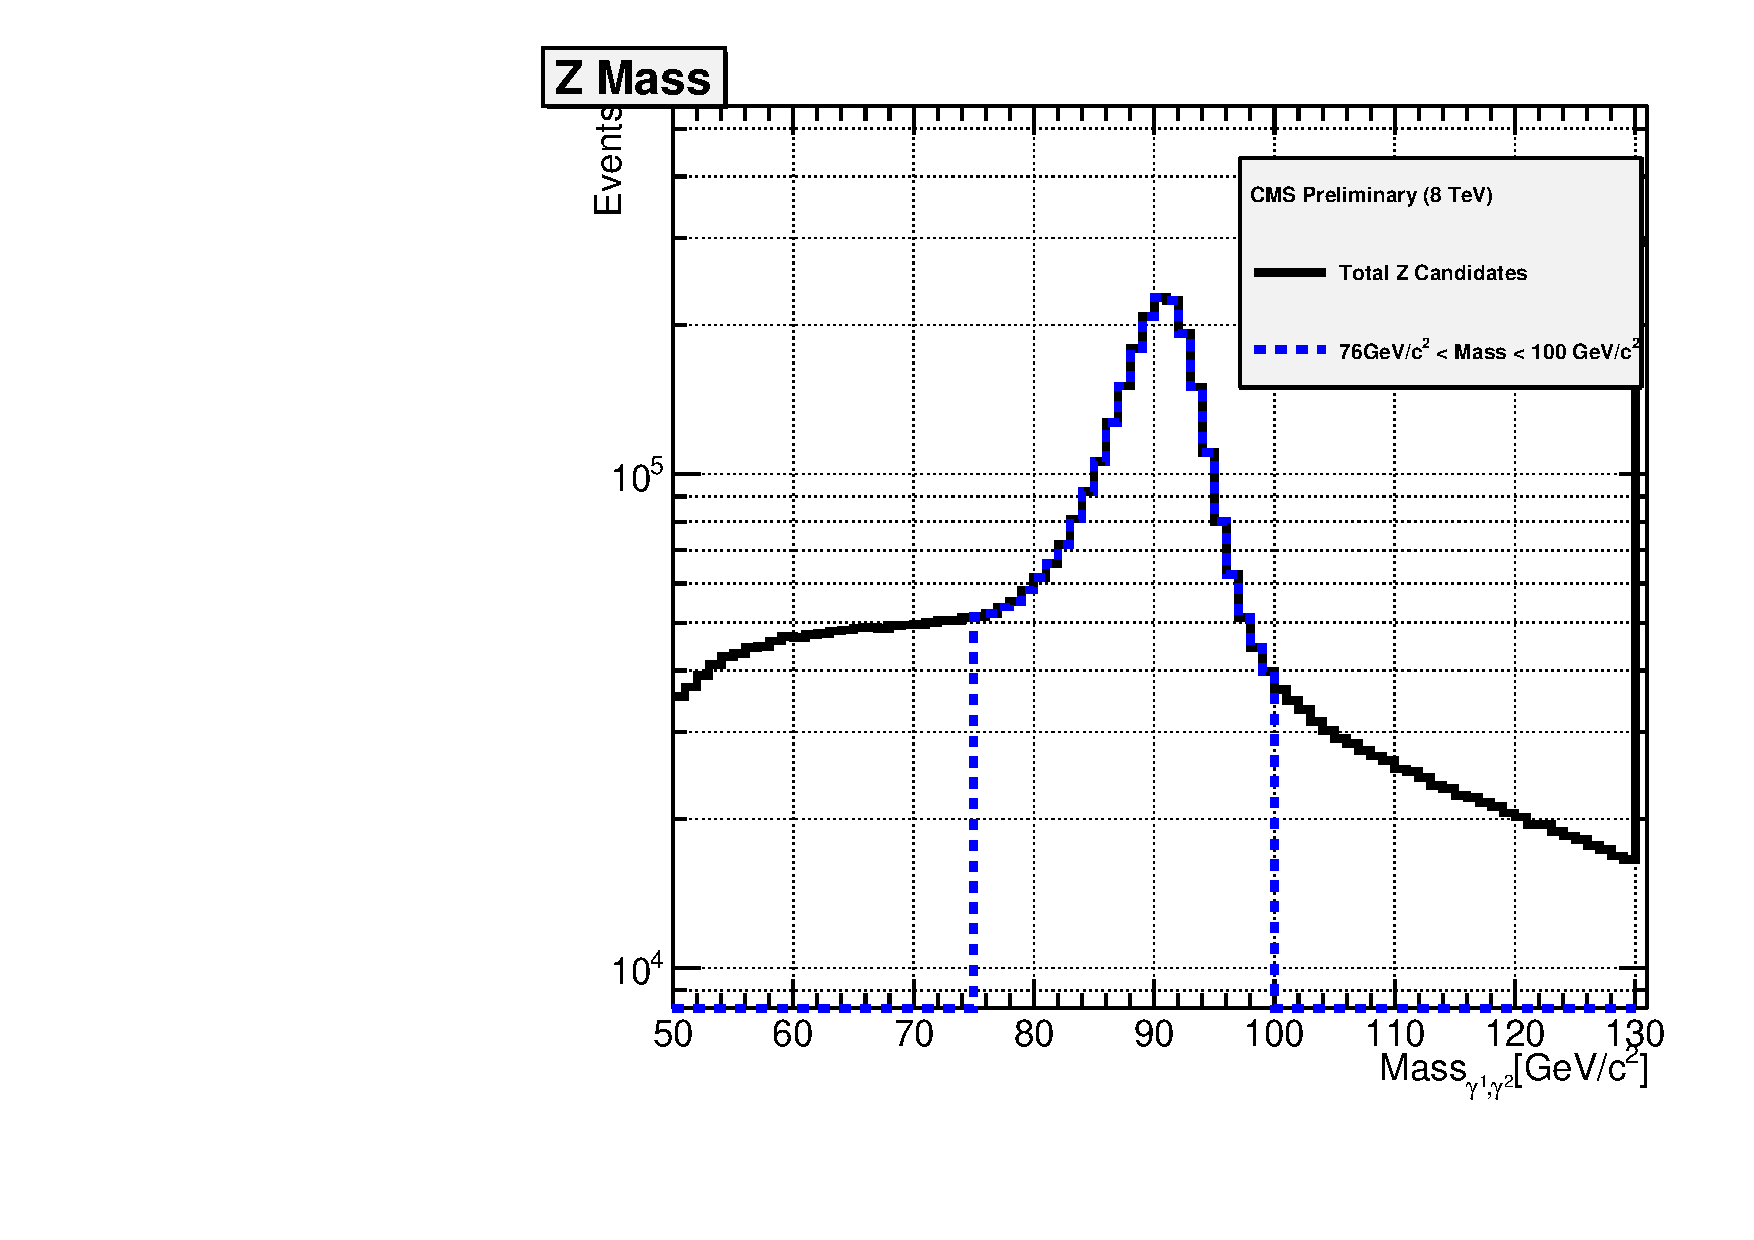
\includegraphics[height=7cm, width=0.5\textwidth]{THESISPLOTS/Z-CandidateOverLay-SignalMass.pdf}
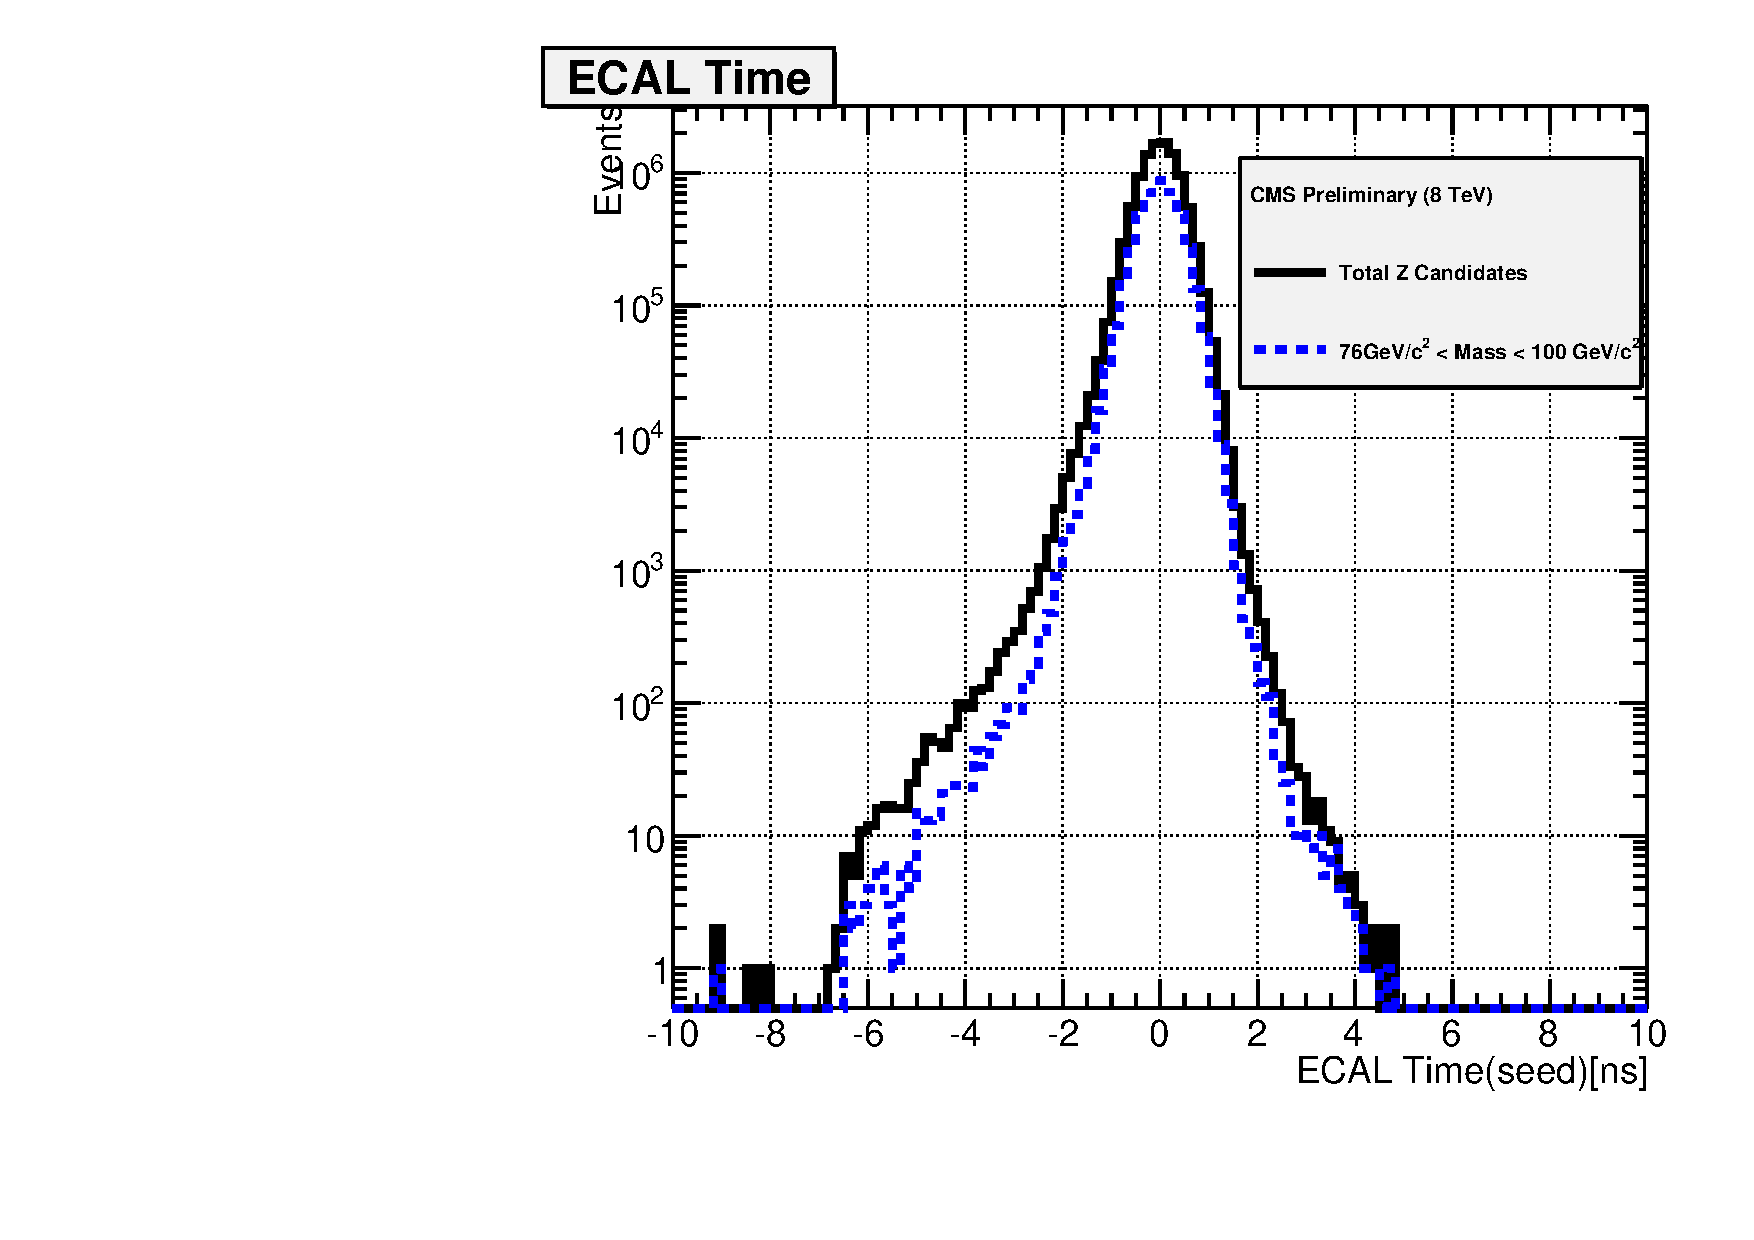
\includegraphics[height=7cm, width=0.5\textwidth]{THESISPLOTS/Z-CandidateOverLay-SignalTime.pdf}}
\mbox{
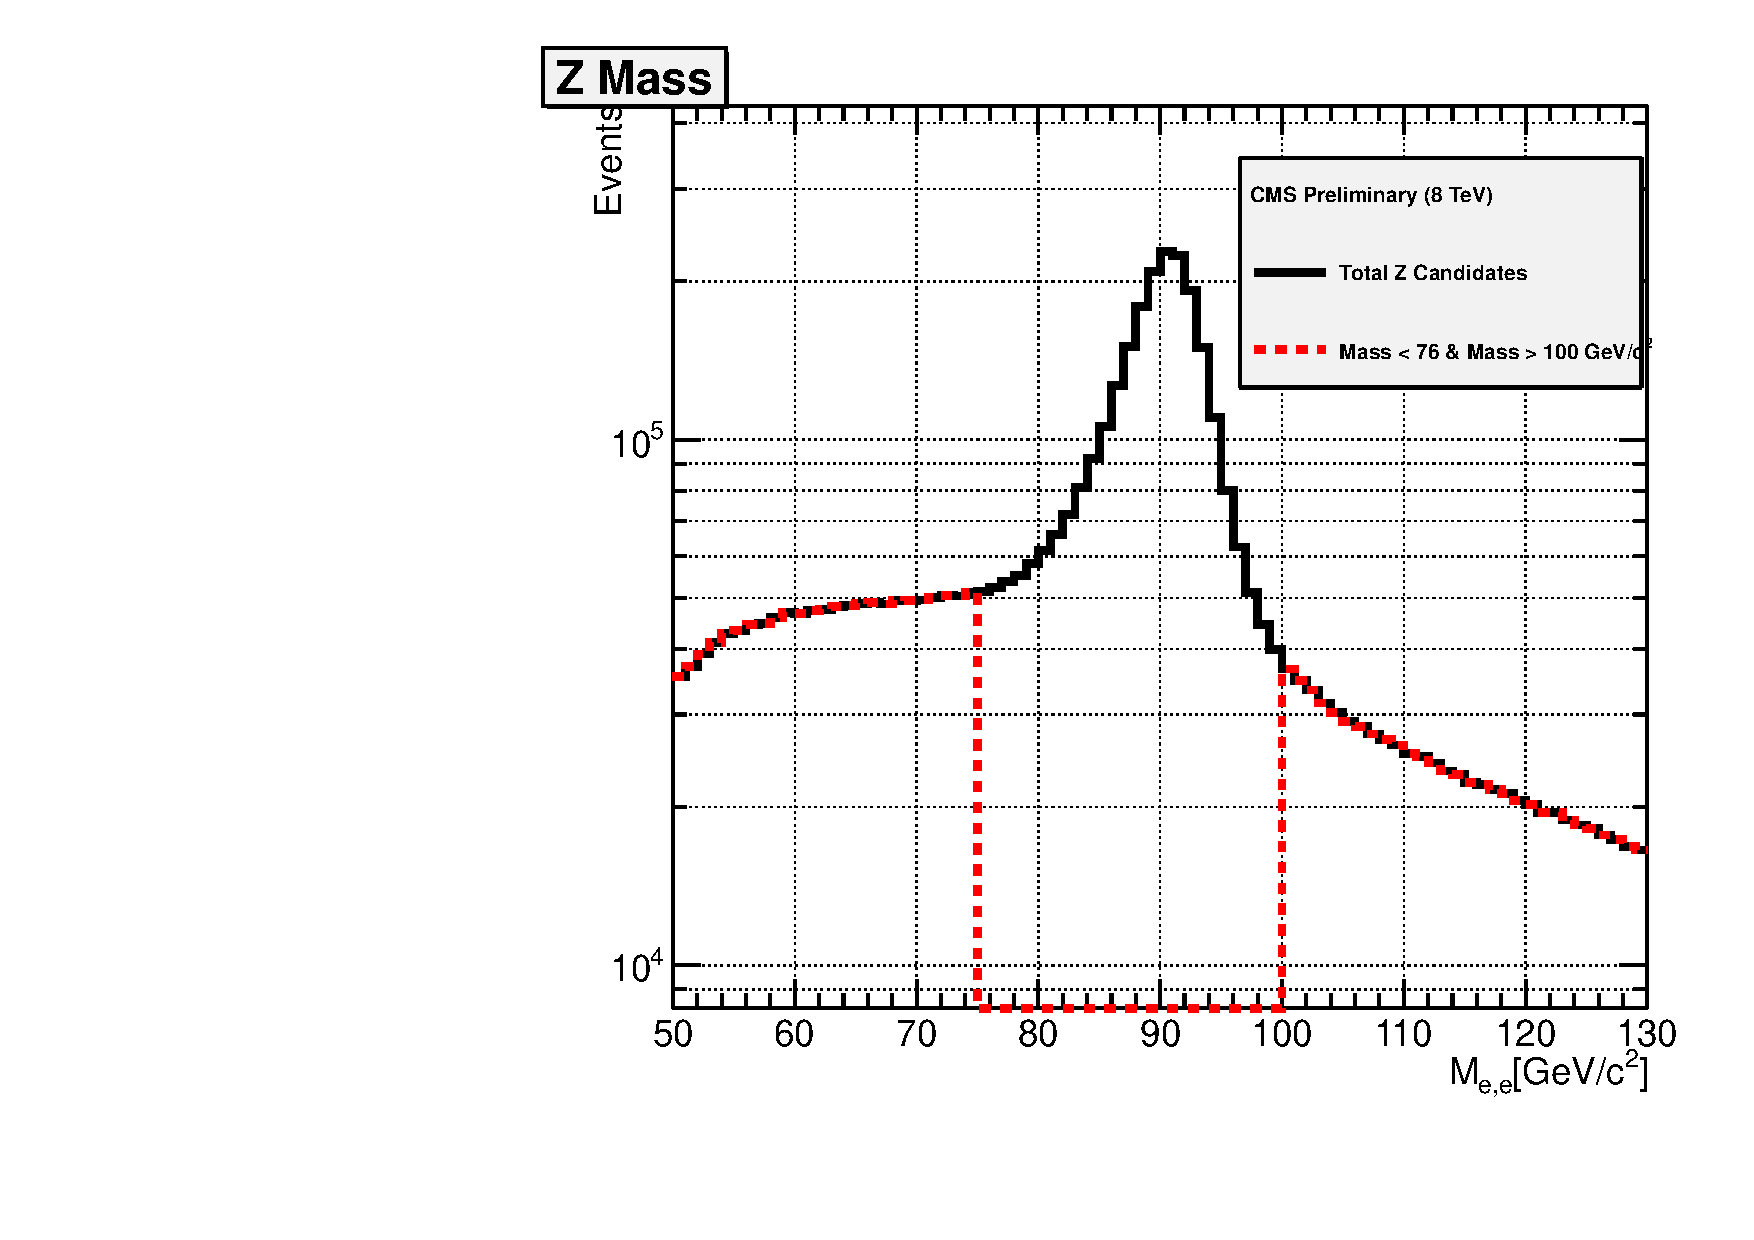
\includegraphics[height=7cm, width=0.5\textwidth]{THESISPLOTS/Z-CandidateOverLay-BackgroundMass.pdf}
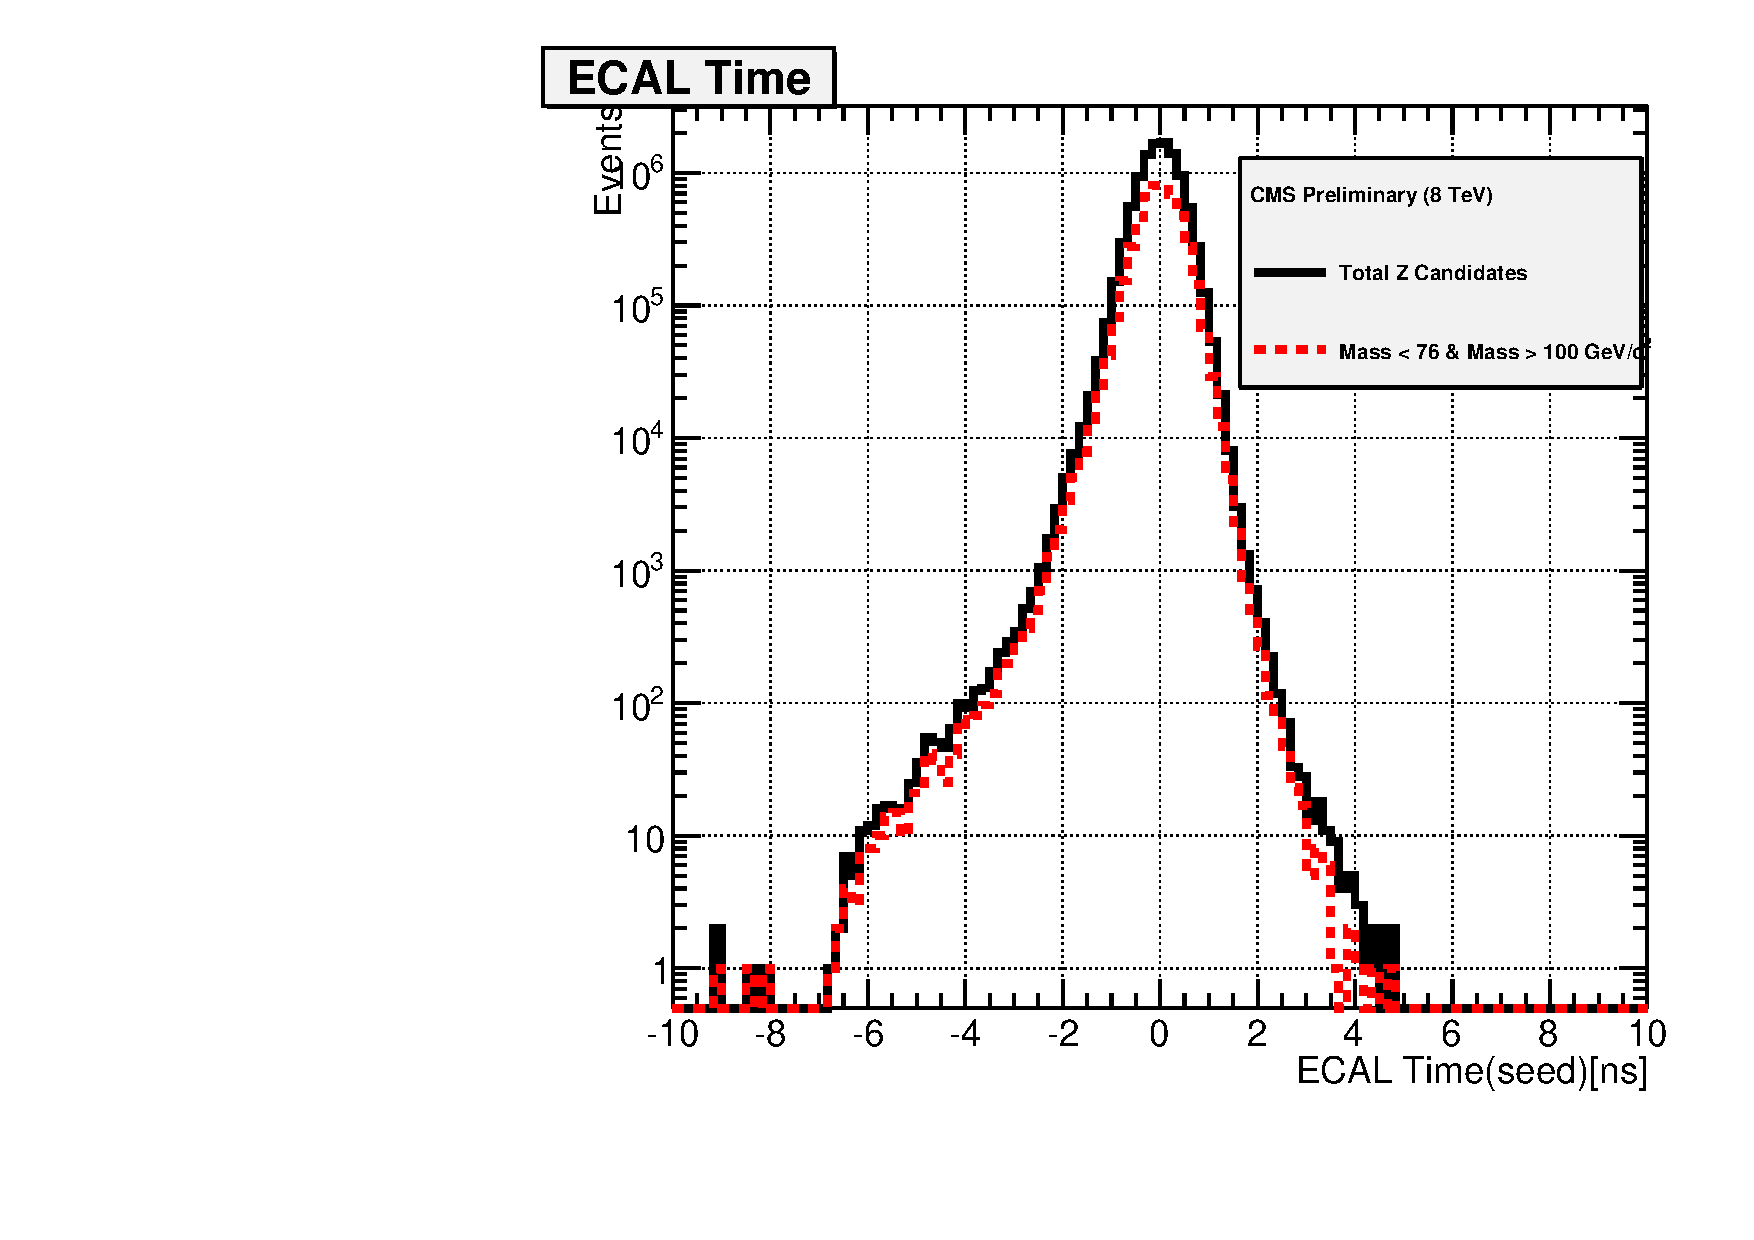
\includegraphics[height=7cm, width=0.5\textwidth]{/home/tensr/Documents/TEN-HEP-PHD-THESIS/PHD_THESIS/PHD/THESISPLOTS/Z-CandidateOverLay-BackgroundTime.pdf}}
\captionof{figure}{Di-electron candidate mass distribution and the time of both electrons for the signal \textcolor{blue}{$76 < m_{Z} < 100$}~\GeVcc $Z$ boson sample(left) and similar distributions from the Control~(\textcolor{red}{$50 < m_{Z} < 76$}~\GeVcc and \textcolor{red}{$ 100 < m_{Z} < 130$}~\GeVcc) sample~(right). Candidates events from the DoubleElectron dataset.}
\label{fig:Zmass}
\end{center}


Using the control sample, we estimate its contribution  using simple scaling which can be understood as an ABCD method into the signal sample as follows:
\begin{itemize}
\item Using a polynomial function, we fit the di-electron candidate mass distribution of the control sample to extract a set of fit parameters,
\item Using the fit parameters, define our polynomial fit function to be used to extract our scaling factor and hence true contribution of the control region events in our signal region which in this case are $Z$ bosons with possible large timing, $|t| > 3$~ns.
\item Scale the control sample events~(electrons time) by this extracted scale factor i.e $$\displaystyle{\mbox{Scale Factor} = \frac{N}{M_{1} + M_{2}}}$$.
\item By subtracting the scaled control sample event timing distribution from the signal sample electron time distribution, we are left with the true $Z$ boson events whose electron time can extend to large time.
\item Comparing the total number of observe electron candidates with $t > 3$~ns to those with time within the required in-time $|t| < 2$~ns using a ratio i.e $ N_{t > 3~ns}/ N_{|t| < 2.0~ns}$ gives us an estimate of the possible genuine collision electromagnetic objects with large timing. 
\end{itemize}  

A simple picture showing the above procedure with distributions is shown in figure \ref{fig:collZ}.

\begin{center}
\centering
\mbox{
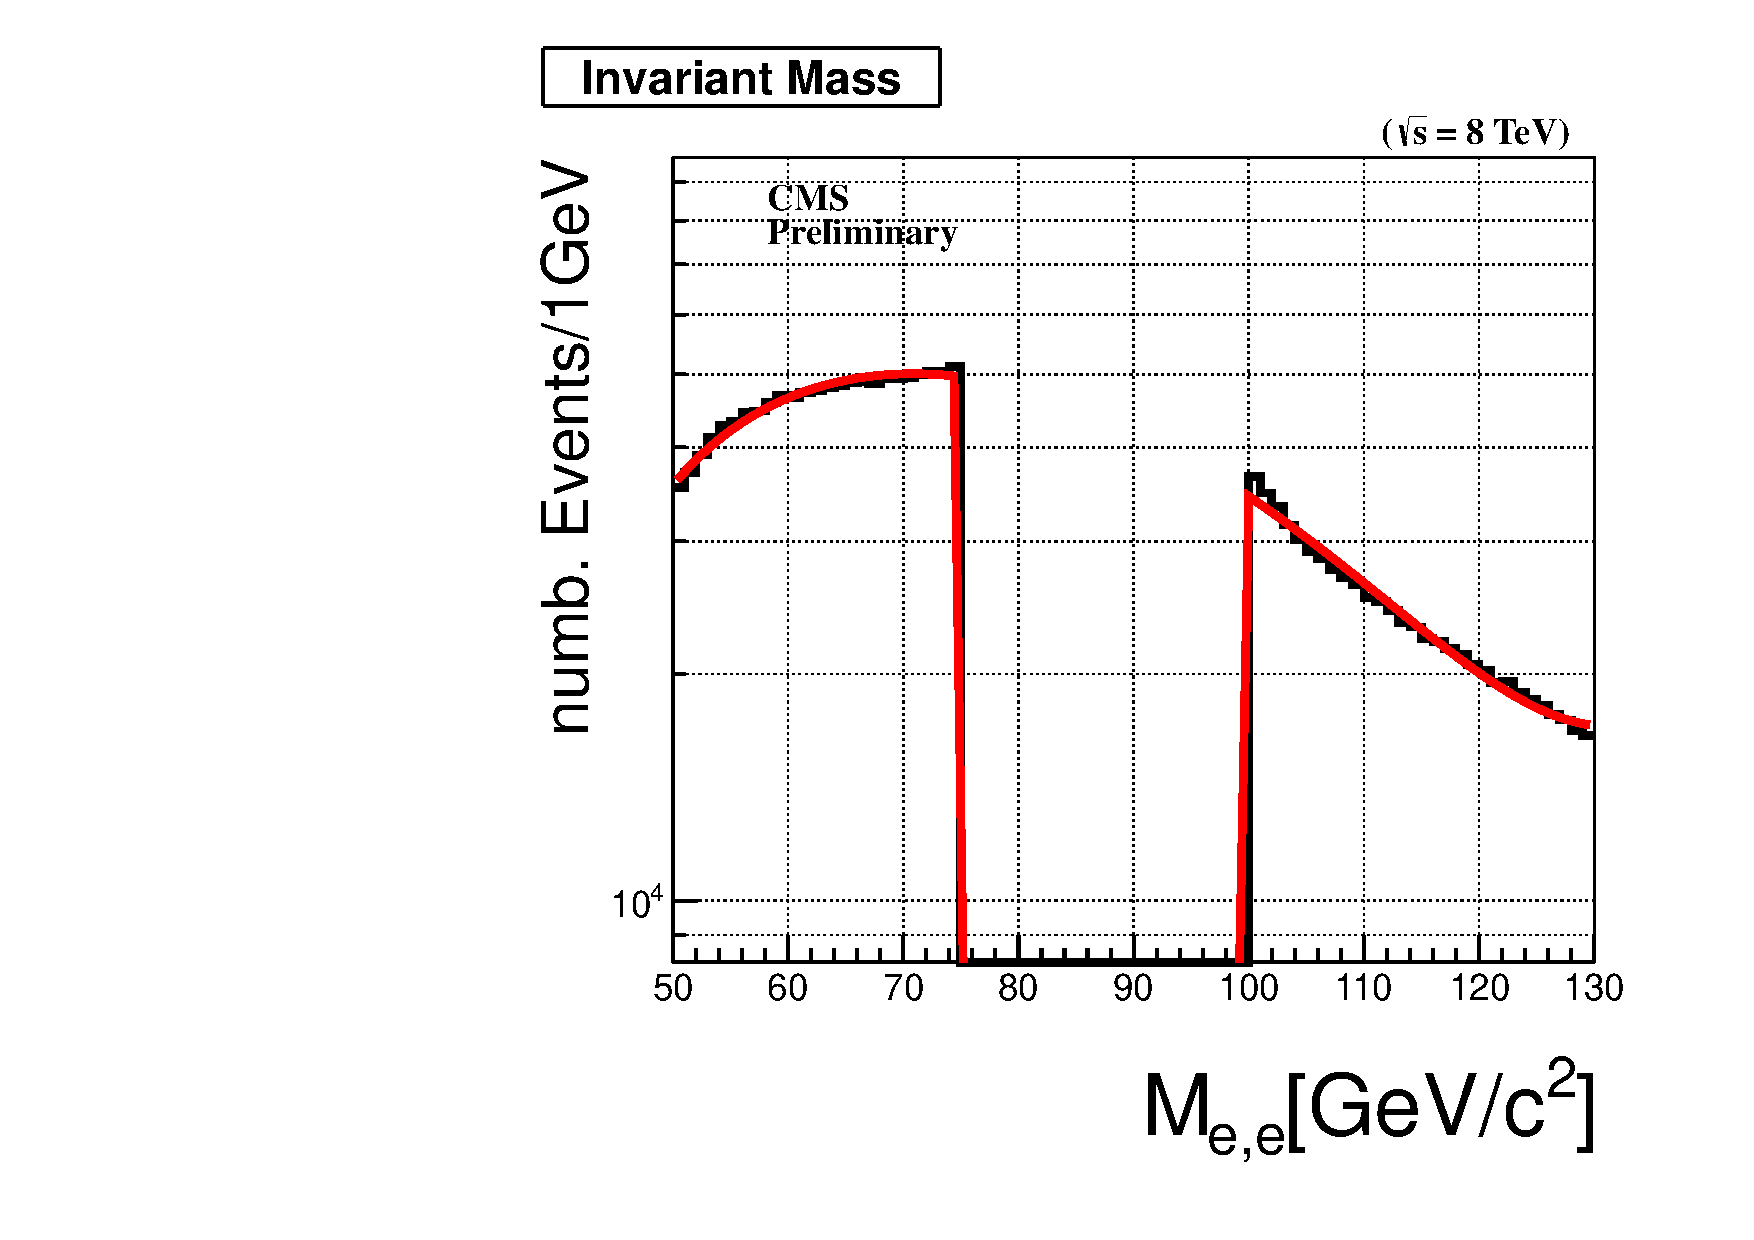
\includegraphics[height=7cm, width=0.5\textwidth]{THESISPLOTS/Uncleaned-di-Photon-ZMass-Fit-DoubleElectron-Run2012A.pdf}
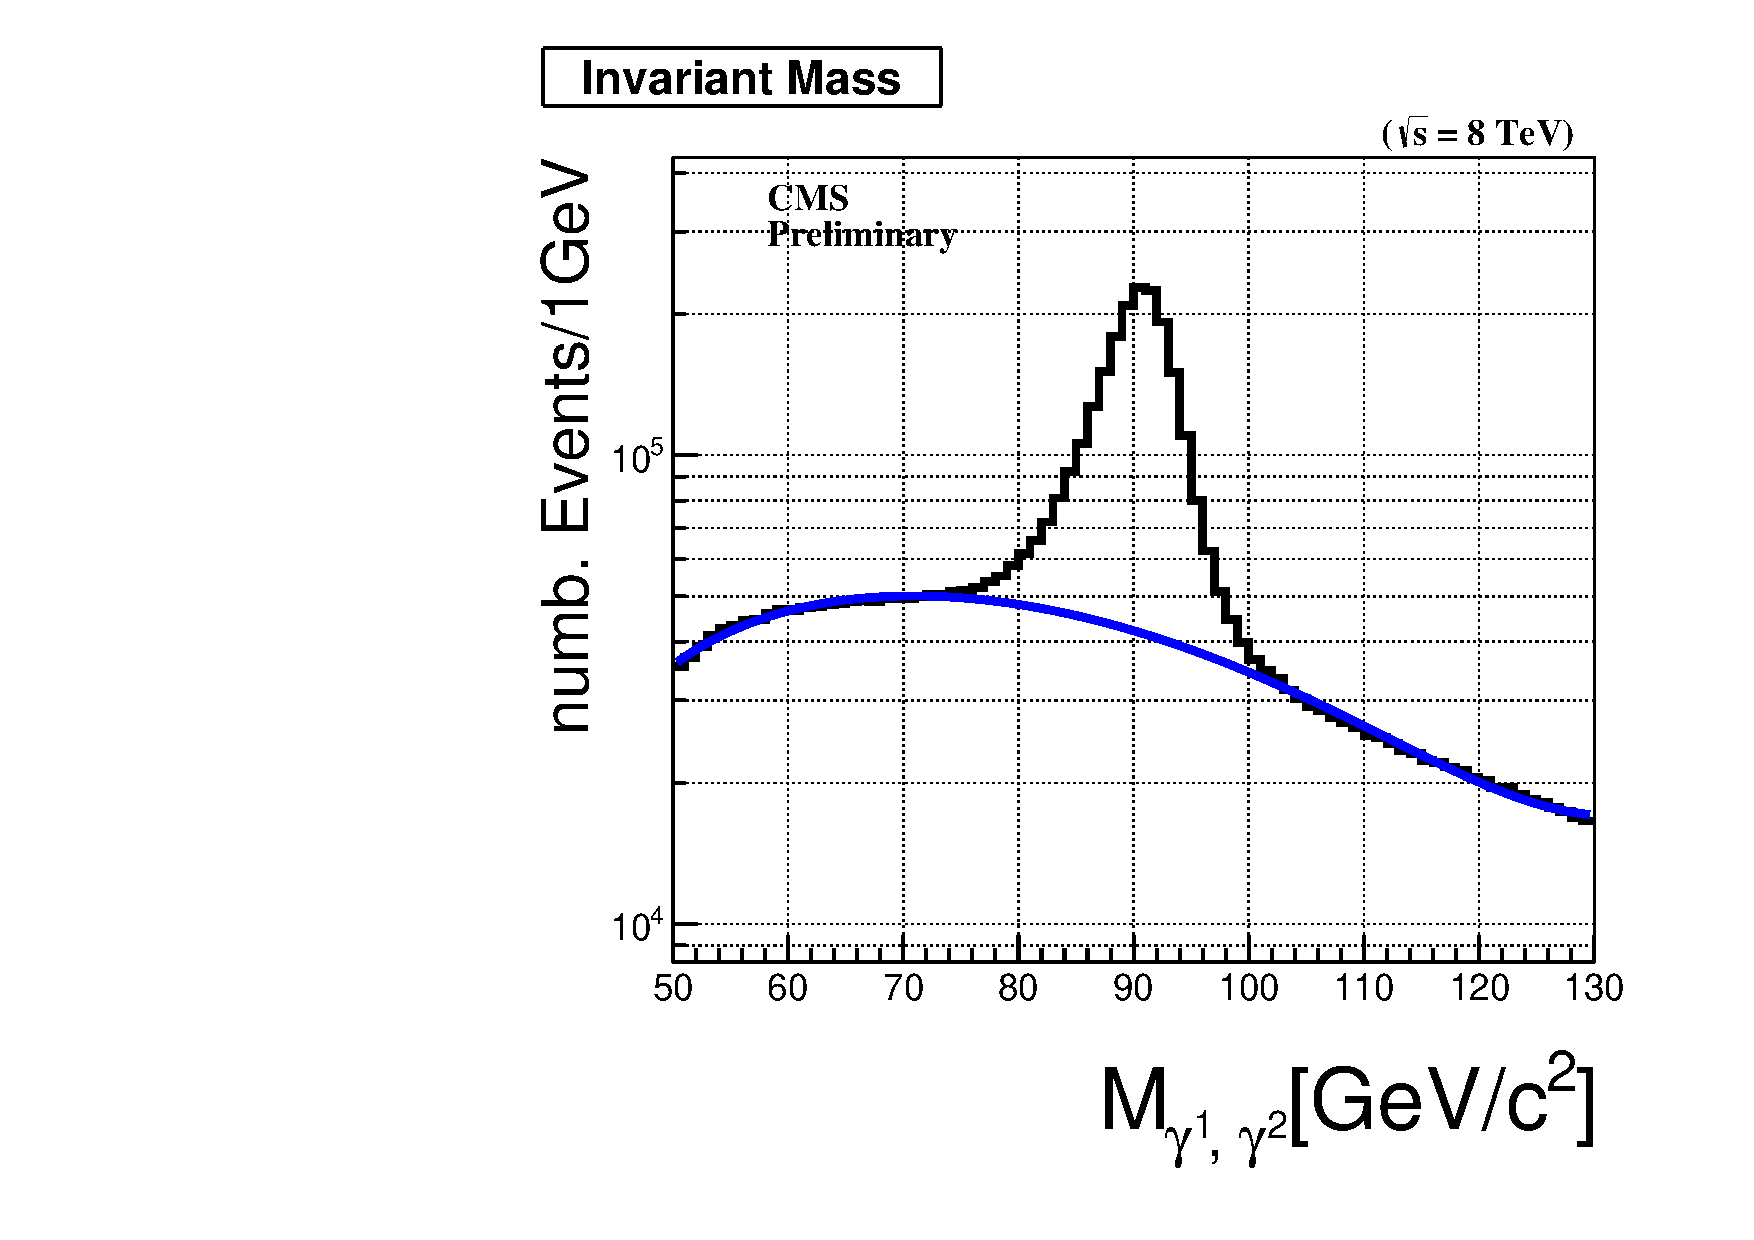
\includegraphics[height=7cm, width=0.5\textwidth]{THESISPLOTS/Background_In_ZMass-From-Di-Photon.pdf}}
\mbox{
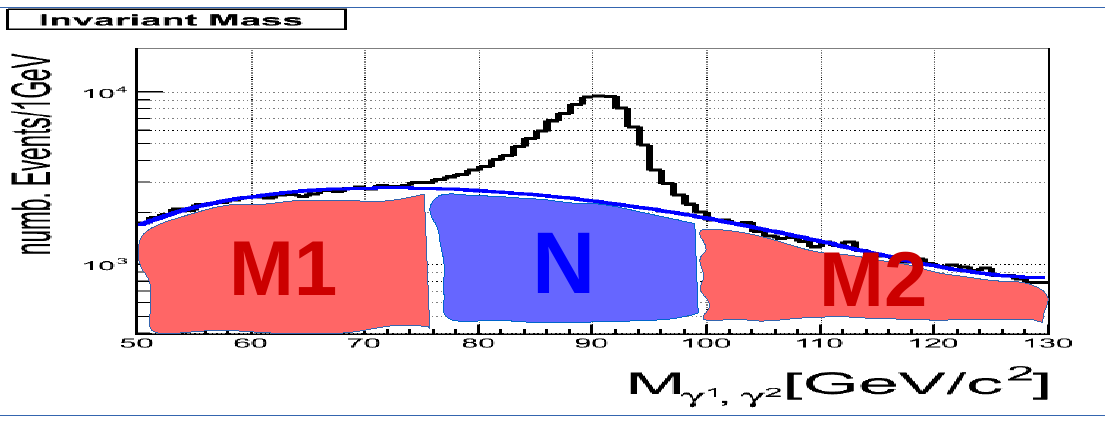
\includegraphics[height=8cm, width=0.8\textwidth]{THESISPLOTS/ZBackground_SF.png}
%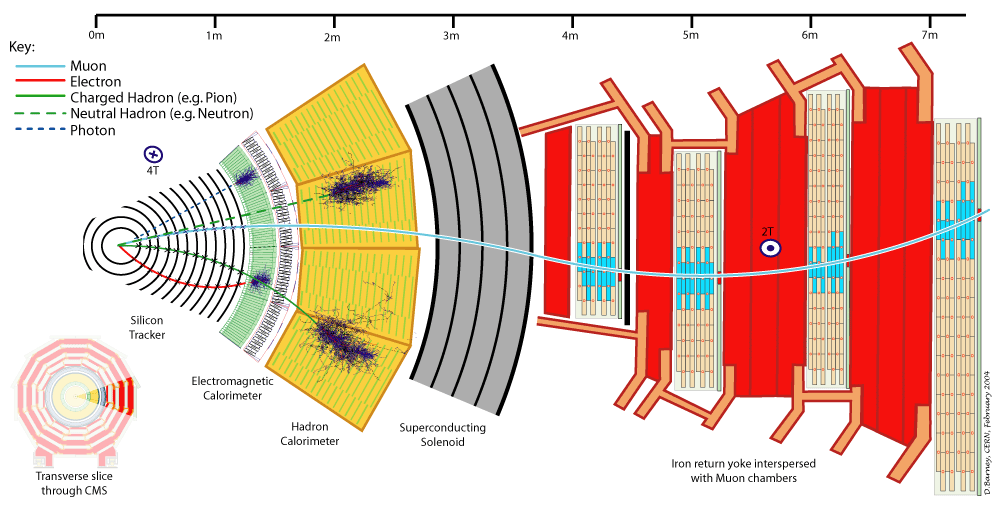
\includegraphics[height=6cm, width=0.5\textwidth]{THESISPLOTS/CMS_Slice.png}
}
\captionof{figure}{\textit{Top}: Control sample~(left) and signal sample~(right) of di-electron candidate mass distribution. \textit{Bottom:} Figure showing definition of scale factor use in estimating the contributions from control sample in signal sample.}
\label{fig:collZ}
\end{center}

The result of the final timing distribution of genuine $Z$ boson events  can be seen in figure \ref{fig:Ztime}. It is not difficult to see that the ratio $ N_{t > 3~ns}/ N_{|t| < 2.0~ns}  < 10^{-5}$ confirming that indeed the contribution  of electromagnetic objects with large timing $t >3$~ns is negligible thus confirming that most collision events contain photons which are mostly in-time, $|t| \leq 2$~ns. A simple cut on the \MET, $\MET > 60$~GeV will further reduce this ratio to $0$ as assumed in our above background estimation.
\begin{center}
\centering
%\mbox{
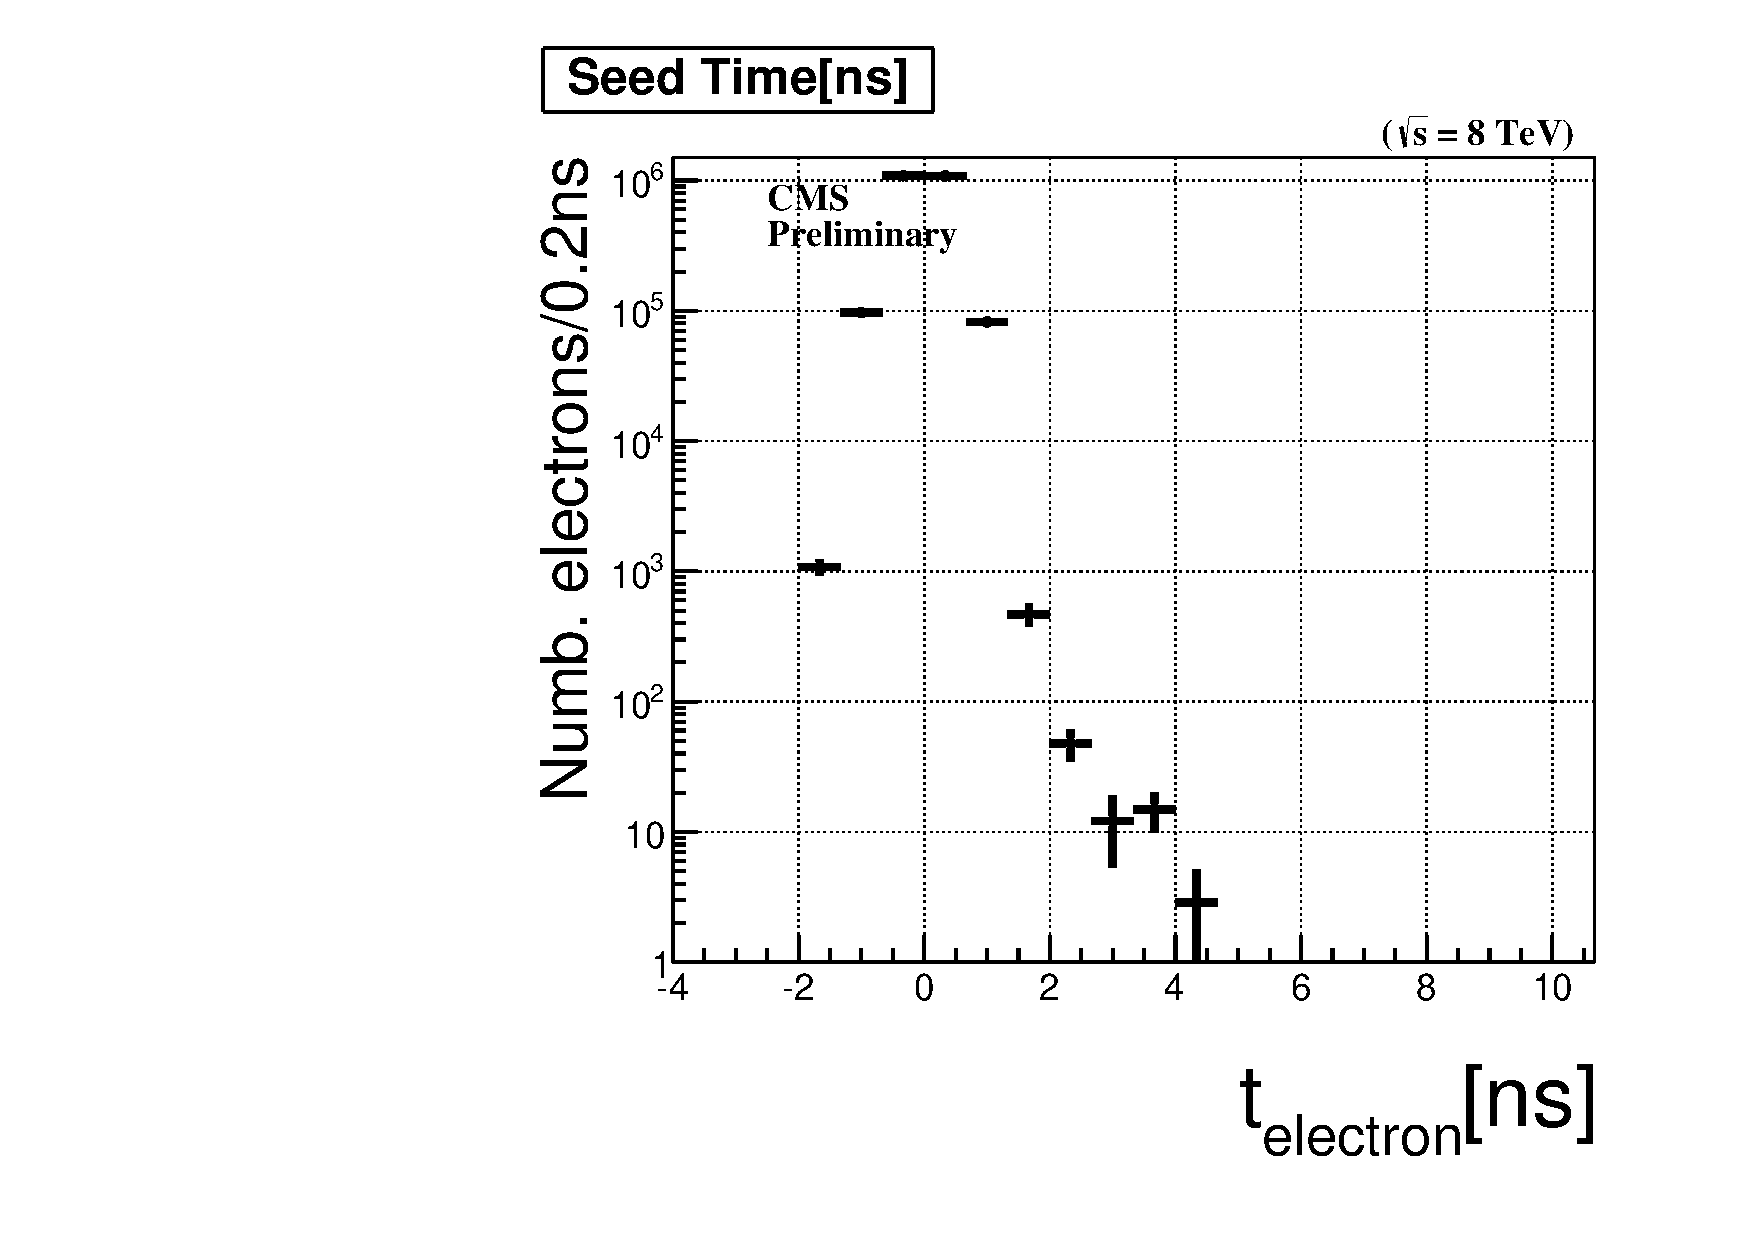
\includegraphics[height=7cm, width=0.7\textwidth]{THESISPLOTS/Seed-Time-From-Uncleaned-di-photon-Mass-Fit-DoubleElectron-Run2012A.pdf}
%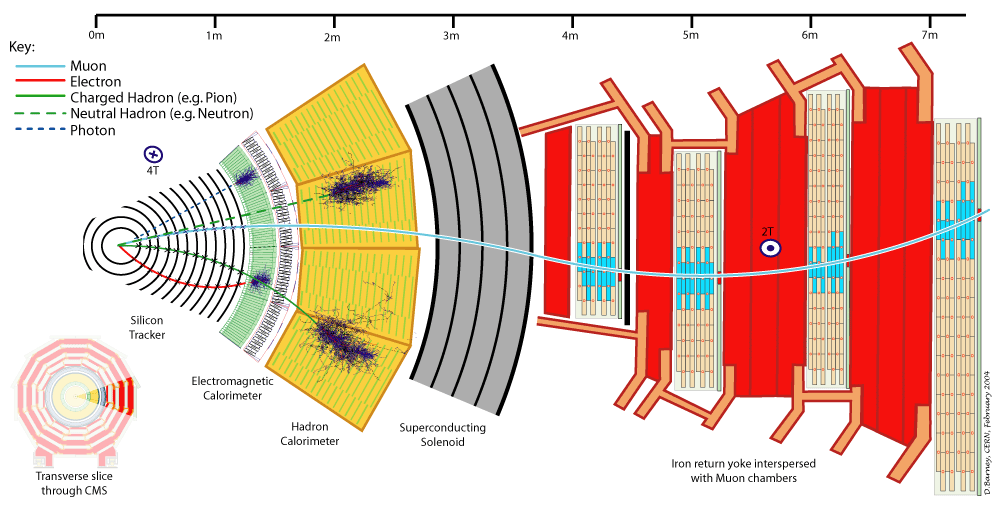
\includegraphics[scale=0.2]{THESISPLOTS/CMS_Slice.png}
\captionof{figure}{Timing distribution of genuine $Z$ bosons after background contribution has been subtracted.}
\label{fig:Ztime}
\end{center}
  


\section{Results}
We have used only the photon arrival time at ECAL to distinguish signal from SM background with our acceptance region being photons with ECAL time $|t| > 3.0$~ns. The final number of events estimated for each background component and observed from data after passing all our selection cuts is shown in table \ref{tab:RESULT}.

\begin{center}
%\begin{table}[ht]
%\renewcommand\arraystretch{1.2}
\centering
\begin{tabular}{c c}
\hline
\bfseries{SM Background/SPS8 GMSB Signal} & \bfseries {Number of Events}\\
\hline
\texttt{QCD~(Collision)}  & $000.00 \pm 0.000$\\
\texttt{Halo Photons}  & $000.00 \pm 0.000$ \\
\texttt{Cosmic Photons} & $000.00 \pm 0.000$ \\
\texttt{Anomalous photons/Spikes} & $000.00 \pm 0.000$\\
\texttt{Total SM background} & $000.00 \pm 0.000$ \\
\hline \hline
\texttt{Data} & $000.00 \pm 0.000$ \\
\hline 
%\texttt{GMSB(SPS8)}~($\Lambda=180$~TeV,$c\tau=93$~mm) & $000.00 \pm 0.000$ \\
%\texttt{GMSB(SPS8)}~($\Lambda=180$~TeV,$c\tau=185$~mm) & $000.00 \pm 0.000$ \\
%\texttt{GMSB(SPS8)}~($\Lambda=180$~TeV,$c\tau=368$~mm) & $000.00 \pm 0.000$ \\
\texttt{GMSB(SPS8)}~($\Lambda=180$~TeV,$c\tau=500$~mm) & $000.00 \pm 0.000$ \\
%\texttt{GMSB(SPS8)}~($\Lambda=180$~TeV,$c\tau=733$~mm) & $000.00 \pm 0.000$ \\
\texttt{GMSB(SPS8)}~($\Lambda=180$~TeV,$c\tau=1000$~mm) & $000.00 \pm 0.000$ \\
%\texttt{GMSB(SPS8)}~($\Lambda=180$~TeV,$c\tau=1076$~mm) & $000.00 \pm 0.000$ \\
%\texttt{GMSB(SPS8)}~($\Lambda=180$~TeV,$c\tau=1444$~mm) & $000.00 \pm 0.000$ \\
\texttt{GMSB(SPS8)}~($\Lambda=180$~TeV,$c\tau=2000$~mm) & $000.00 \pm 0.000$ \\
%\texttt{GMSB(SPS8)}~($\Lambda=180$~TeV,$c\tau=2161$~mm) & $000.00 \pm 0.000$ \\
\texttt{GMSB(SPS8)}~($\Lambda=180$~TeV,$c\tau=3000$~mm) & $000.00 \pm 0.000$ \\
\texttt{GMSB(SPS8)}~($\Lambda=180$~TeV,$c\tau=6000$~mm) & $000.00 \pm 0.000$ \\
\texttt{GMSB(SPS8)}~($\Lambda=180$~TeV,$c\tau=12000$~mm) & $000.00 \pm 0.000$ \\
\hline \hline
\end{tabular}
\captionof{table}{Final number of events estimated for each background and the number of events passing out event selection and acceptance criteria.}
\label{tab:RESULT}
%\end{table}
\end{center}



\subsection{Systematics Studies}
The different sources of systematics which affect this analysis and the estimated contribution of each identified systematics is used in the calculation of the upper limit on observed signal cross-section is shown in table \ref{tab:SYST}.
The systematic uncertainty on luminosity measurement has the recommended value of $2.2$\%. The uncertainty for the jet energy scale correction has also been measured using the standard CMSSW tool by \cite{JES}. The uncertainty on the photon energy scale in barrel was estimated to be 1.0\% and based on the final-state radiation~(FSR) in $Z\rightarrow \mu\mu\gamma$ events \cite{PES}. The uncertainty from pardon density functions~(PDF) evaluated using the re-weighting technique and Master equation of CTEQ65 model set described in \cite{PDF}. The uncertainty on the \MET resolution uses a conservative estimate from \cite{METRES}. The uncertainty on the ECAL timing obtained be comparing the peak in the timing distribution between $\gamma +$ jet sample and data events with time $|t| < 2$~ns to be of the order of 200~ps per event and from a study of high \pt photons beyond gain transitions and has been agreed by ECAL DPG to be a conservative estimate. Another important source of systematics is in the selection of the background control samples and estimation and individual systematics in the tagging and miss-tagging of non-collision background and also with the estimation of background contributions from collisions. All these separate systematics contributions have been combined into a single background estimation systematics referred to as background estimation systematics. The summary of every systematics in shown in table \ref{tab:SYST}. 



\begin{center}
%\begin{table}[ht]
%\renewcommand\arraystretch{1.2}
\centering
\begin{tabular}{c c}
\hline
\bfseries{Source} & \bfseries {Uncertainty on $\sigma^{Exp}_{UL}$}(\%)\\
\hline
\texttt{Photon energy scale}~(1.0\%)  & $< 3.0$\% \\
\texttt{Jet energy scale}  & $< 0.05$\% \\
\texttt{Jet energy resolution}~(10\%) &$ < 1.90$\% \\
\texttt{PDF uncertainty}~(10\%) & $< 1.70$\% \\
\texttt{\MET resolution}~(10\%) & $ <2.8$\%  \\
\texttt{ECAL time uncertainty}~(0.5~ns) & $<5.0$\% \\
\hline
\texttt{Background estimation uncertainty}~(20.0) &$<10.0$\% \\
\hline 
\texttt{Luminosity}~(4.5\%) & $< 2.2$\% \\
\hline
\end{tabular}
\captionof{table}{Summary of systematic uncertainties on the signal~(top), background~(middle) and machine~(bottom) as used in the $\sigma_{UL}$ calculation.}
\label{tab:SYST}
%\end{table}
\end{center}



\label{Search_Analysis_chapter}